% paper-v4.tex -- copia de paper-v3.tex (NAO tocar em paper-v3.*) com o
% teorema de forcing incorporado.
% v4: teorema de forcing incorporado (15o parecer). Fonte da verdade matematica:
% 06-notas/t2-prova/teorema-forcing-draft.tex; pareceres 14 e 15 em
% 05-experimentos/t2-n-neuronios/parecer-1{4,5}.md.
% Novidades de v4: Teorema 6 (forma forcing) na secao 3.1; secao 3.6 com a
% verificacao numerica do forcing; corolario da transferencia na secao 4;
% Apendice B com a prova completa; escopo da secao 1 em tres niveis (P1)-(P3).
% Estado v3 (base): 43 paginas, 7 figuras, 4 tabelas.
% Estado atual: 65 paginas, 7 figuras, 6 tabelas; 0 undefined, 0 overfull,
% 0 float-too-large em 3 passes de pdflatex.
% arXiv, campo Comments (C17): "65 pages, 7 figures, 6 tables. Comments welcome."
% Versao canonica arXiv (autor visivel). Submissao TMLR = conversao p/ tmlr.sty
% ANONIMIZADA (ver 06-notas/paper/submissao-checklist.md).
% Categoria primaria math.DS, cross-list cs.LG.
% Convencoes da casa fixadas: Psi = quadratura log u + u (Phi reservado para a
% parametrizacao); H = horizonte de treino (tempo no fluxo, passos no experimento);
% T = SO temperatura do SGLD; \Ar = area acumulada (neuronios seguem A e B).
\documentclass[11pt]{article}
\usepackage{amsmath,amssymb,amsthm}
\usepackage[text={6in,8in},centering]{geometry}   % F22: limite SIADS
\usepackage{graphicx}
\usepackage{url}
\usepackage{array}
\usepackage{booktabs}
\usepackage{microtype}
\usepackage{aliascnt}
\usepackage{algorithm}
\usepackage{algorithmic}
\usepackage[colorlinks=true,linkcolor=blue,citecolor=blue,urlcolor=blue]{hyperref}
\usepackage[nameinlink]{cleveref}                 % C4: nada de "Thm."/"Fig."

% B13: contador COMPARTILHADO, sequencia unica (estilo SIAM). Os contadores
% aliased (aliascnt) mantem a sequencia unica E preservam o tipo de cada
% ambiente, para o cleveref imprimir "Lemma 5" e nao "theorem 5".
\newtheorem{theorem}{Theorem}
\newaliascnt{lemma}{theorem}
\newtheorem{lemma}[lemma]{Lemma}
\aliascntresetthe{lemma}
\newaliascnt{proposition}{theorem}
\newtheorem{proposition}[proposition]{Proposition}
\aliascntresetthe{proposition}
\newaliascnt{corollary}{theorem}
\newtheorem{corollary}[corollary]{Corollary}
\aliascntresetthe{corollary}
\theoremstyle{definition}
\newaliascnt{definition}{theorem}
\newtheorem{definition}[definition]{Definition}
\aliascntresetthe{definition}
\newtheorem*{theorem*}{Theorem}
\theoremstyle{remark}
\newaliascnt{remark}{theorem}
\newtheorem{remark}[remark]{Remark}
\aliascntresetthe{remark}

% C4: nomes por extenso; equacao sem a palavra "eq." (IOP 4.4).
\crefname{algorithm}{Algorithm}{Algorithms}
\Crefname{algorithm}{Algorithm}{Algorithms}
\crefname{theorem}{Theorem}{Theorems}
\Crefname{theorem}{Theorem}{Theorems}
\crefname{lemma}{Lemma}{Lemmas}
\Crefname{lemma}{Lemma}{Lemmas}
\crefname{proposition}{Proposition}{Propositions}
\Crefname{proposition}{Proposition}{Propositions}
\crefname{definition}{Definition}{Definitions}
\Crefname{definition}{Definition}{Definitions}
\crefname{remark}{Remark}{Remarks}
\Crefname{remark}{Remark}{Remarks}
\crefname{equation}{}{}
\Crefname{equation}{}{}
\crefname{figure}{Figure}{Figures}
\Crefname{figure}{Figure}{Figures}
\crefname{table}{Table}{Tables}
\Crefname{table}{Table}{Tables}
\crefname{section}{Section}{Sections}
\Crefname{section}{Section}{Sections}
\crefname{appendix}{Appendix}{Appendices}
\Crefname{appendix}{Appendix}{Appendices}

\newcommand{\R}{\mathbb{R}}
\newcommand{\thit}{t_{\mathrm{hit}}}
\newcommand{\texit}{t_{\mathrm{exit}}}
\newcommand{\trel}{t_{\mathrm{release}}}
\newcommand{\Ar}{\mathcal{A}}                      % area acumulada
\newcommand{\Tep}{T_{\mathrm{ep}}}   % duracao do episodio (NAO o horizonte H)
\newcommand{\hyb}{\mathrm{hyb}}
% v4: macros do teorema de forcing (portadas de t2-prova/teorema-forcing-draft.tex).
\newcommand{\tcross}{t_{\mathrm{cross}}}
\newcommand{\res}{\mathrm{res}}

% E6: reenunciado de lema no apendice, com a numeracao original e o mesmo
% corpo do texto principal; as equacoes reimprimem o numero de origem via
% \tag{\ref{...}}, de modo que nada e renumerado nem redefinido.
\newenvironment{lemmarep}[2]{%
  \par\medskip\noindent\textbf{Lemma \ref{#1} (#2).}\itshape\ \ignorespaces}%
  {\par\medskip}

% Slot para os cinco estimandos da etapa-5. Enquanto o argumento for vazio, nada
% e impresso; quando o confirmatorio fechar, basta preencher cada \eresult{}.
\makeatletter
\newcommand{\@eresempty}{}
\newcommand{\eresult}[1]{%
  \def\@erestmp{#1}%
  \ifx\@erestmp\@eresempty\else\ \textit{Result:}~#1\fi}
% E6: as hipoteses (H0')-(H5') do teorema de forcing sao referenciadas no mesmo
% registro tipografico de (H1)-(H4) da secao 3, isto e via \eqref. Elas nao
% podem virar um align (o corpo de (H4') contem prosa e um display proprio),
% entao damos a cada item um alvo de \label cujo texto impresso e o rotulo da
% hipotese; \eqref{H0p} imprime entao "(H0')" tal como \eqref{H1} imprime "(H1)".
% Nao mexe no contador de equacoes: nada e renumerado.
\newcommand{\hyplabel}[2]{%
  \phantomsection
  \protected@edef\@currentlabel{#1}\label{#2}}
\makeatother

\title{An entry--exit law for the resurrection of dead neurons
under smoothed ReLU activation}
% B3 resolvido: nome/e-mail/cidade confirmados pelo autor em 2026-07-26: forma canonica do nome, endereco de e-mail a divulgar,
% e cidade a declarar. O que esta abaixo satisfaz a norma (nome + afiliacao +
\author{Leonardo Caloi Santos\thanks{Independent researcher, Maring\'a,
Paran\'a, Brazil. \texttt{leonardo@ventros.com.br}.}}
\date{July 26, 2026}

\begin{document}
\maketitle

\begin{abstract}
A neuron dies when its pre-activation margin is negative on every datum, and
under hard ReLU its gradient is exactly zero, so it never returns. In the
sharp-activation limit of a shallow softplus network under gradient flow the
dynamics is instead hybrid with memory: we prove that the dead unit is
released exactly when the signed time integral of the residual excluding it
returns to zero, at rate $O(\log\beta/\beta)$ and with a first-order release
coefficient in which the arrival speed has cancelled. A sweep of 600
instances isolates 57 satisfying the hypotheses; the law holds in all 57,
median relative error $2.7\%$, coefficients spanning a factor of 20.
The law is a statement about the forcing: a second theorem extends it to any
affine live subsystem with $m$ units, with constants uniform to $O(\sqrt m)$. A
pre-registered ladder follows, ending in two confirmatories. A 400-run MLP
reproduces resurrection, the area in fact turning positive in 13 of 16 returns,
hard ReLU structurally zero. A transformer confirmatory of 800 pre-registered
runs transfers the class to the feed-forward block through the unit's own
channel ($\hat p=0.440$) and reproduces a second, upstream channel in all four
arms: hard-ReLU units return 20 of 100, against 0 with attention frozen.
\end{abstract}

\noindent\textbf{Keywords:} entry--exit function; geometric singular
perturbation; dead neurons; smoothed ReLU; gradient flow; loss of plasticity.

\smallskip
\noindent\textbf{MSC 2020:} Primary 34E15; Secondary 34A36, 68T07.

\section{Introduction}\label{sec:intro}

Write $\Phi:\mathcal{W}\to\mathcal{F}$ for the parametrization of a network and
$J=D\Phi$ for its Jacobian. A neuron whose pre-activation margin is negative on
every datum contributes an identically zero column to $J$: it sits on a stratum
of the singular locus where $J$ drops rank. This is exact for ReLU and
exponentially thin for softplus-$\beta$; it does not hold for GELU at all, whose
output is nonzero for every finite negative margin (\cref{sec:transformer-gelu}).
Under a hard ReLU the gradient of the
loss in the directions of that unit is exactly zero, so the stratum is absorbing.
A dead unit stays dead. This is the mechanism behind the empirically documented
dormant-neuron and loss-of-plasticity
phenomena~\cite{Sokar23,Lyle23,Dohare24}. The question of this paper is what
replaces the absorbing stratum when the activation is smoothed, as it is in every
softplus or GELU~\cite{HG16} network actually trained.

Our answer is an exact gating law and its numerical arc.

\begin{theorem*}[informal]
In the sharp-activation limit of the smoothed flow, a dead unit does not sit on
an absorbing stratum: it freezes and is released exactly when the signed time
integral of the residual that excludes it returns to zero. The stratum is a
memory gate rather than a trap. The convergence to that hybrid limit is uniform
away from the two switching instants, at the rate $O(\log\beta/\beta)$ in the
activation stiffness $\beta$, and the release time carries the first-order
coefficient $-1/(cR(\texit))$, in which the arrival speed has cancelled: the
residual at death drops out, while the coefficient still depends on the datum
constant $c$ and on the residual at the exit. The precise statement is
\cref{thm:main}.
\end{theorem*}

\paragraph{Scope of the proved object.} \Cref{thm:main} covers the minimal
case: one dead unit, one live unit, one active datum at a time, a \emph{fixed}
readout and a one-dimensional input. \Cref{thm:forcing} removes the second of
those restrictions --- the live side may be any affine subsystem of any order
$m$ --- and in doing so it changes the status of the transfer from the proved
object to the measured one, which a statement about two neurons alone would
leave simply empirical. The honest statement is a gradation in three levels, and
we keep the levels separate throughout.

\begin{enumerate}
\item[(P1)] \textbf{Proved, affine class.} For a network with fixed readout
whose live units keep a constant activation pattern on the window, the
entry--exit law holds for every $m$, with constants growing at most like
$\sqrt m$ and threshold $\beta_0=O(m)$ (\cref{thm:forcing,prop:beta0}). Nothing
here is conjectural and nothing is fitted.
\item[(P2)] \textbf{Corollary under hypotheses verifiable a posteriori.} For an
MLP of the affine class --- readout held fixed --- the law at a given
resurrection episode is a \emph{corollary} of \cref{thm:forcing}, not an
analogy, once \eqref{H1p}--\eqref{H2p} are checked on the hybrid trajectory and the
window of \eqref{H4p} is identified. Both checks are one hybrid integration
(\cref{sec:forcing-numerics}); neither is guaranteed a priori by any
initialization criterion we know: in our sweeps the acceptance rate is about
$3\%$ of random draws in the NTK-readout family and about $20\%$ ($179/900$) in
the unit-readout family.\footnote{Four acceptance rates appear in this paper
and each is a property of its own prior and screen, not of the hypotheses:
$9.5\%$ ($57/600$) for the two-neuron sweep of \cref{sec:sweep}, $26\%$
conditional on a death inside the detector window, and the $3\%$/$20\%$
per-family rates of the $m$-sweep. They are not comparable to one another.}
\item[(P3)] \textbf{Empirical.} A trainable readout $v_k$, which is what the
experiments of \cref{sec:experiments} use and what takes the live field outside
the gradient-of-a-convex-function class; several data active at once; and the
transformer of \cref{sec:transformer}. For these the transfer is measured, not
deduced, and we say so wherever a number from them is reported.
\end{enumerate}

The contributions are:

\begin{itemize}
\item \textbf{A theorem (\cref{sec:theorem,thm:main}).} In the sharp limit
$\beta\to\infty$ of a shallow softplus network under gradient flow, the death and
resurrection of a neuron is the entry--exit problem of a slow--fast
system~\cite{DMS16}: the dead unit freezes and reactivates when $\int R\,dt=0$,
where $R$ is the residual excluding that unit. The uniform rate is
$O(\log\beta/\beta)$ and the release time carries the first-order coefficient
$-1/(cR(\texit))$, from which the arrival speed has cancelled. The proof is
organized as six lemmas (\cref{app:lemmas}), each with an independent executable
symbolic or numerical verification. A consequence of the same construction is
that the two limit orders, smooth-then-sharp against the pointwise
generalized-gradient flow, do not commute (\cref{sec:noncomm}): the field-first
order is the frozen branch of Eberle, Jentzen, Riekert and Weiss~\cite{EJRW23},
our flow-first limit resurrects, and the autodiff convention that fixes the
branch is discussed in \cref{sec:related}. For the erf smoothing we verify
numerically that the release criterion is unchanged; the proof is written for
softplus, and GELU is outside the class because its derivative is non-monotone.

\item \textbf{A second theorem: the law belongs to the forcing
(\cref{sec:forcing,thm:forcing}).} The residual $R$ is treated as a
\emph{prescribed forcing} and the live side is allowed to be any affine
subsystem of order $m$ --- any number of live units with a constant activation
pattern and a fixed readout --- instead of the single live neuron of
\cref{thm:main}. The same law holds, with the same first-order coefficient
$-1/(cR^{\hyb}(\texit))$, which is structurally free of $m$. The estimate that
carries the live subsystem is replaced by an energy estimate using only
$G_B\succeq0$, so the constant $M_2=C_fC_4/c$ carries no factor $e^{L_BH}$ and
there is \textbf{no restriction of the form $m\cdot H$ small}: every explicit
constant is uniform to $O(\sqrt m)$ and the threshold is $\beta_0=O(m)$
(\cref{prop:beta0}), both at fixed forcing. The proof is
\cref{app:forcing}; the verification, on $66+23+67$ instances and a joint
regression over $133$, is \cref{sec:forcing-numerics}.

\item \textbf{A sweep from one instance to a law (\cref{sec:sweep}).} Every
constant is verified on a reference two-neuron instance, and a sweep of 600
random instances then tests the release law against the dynamics on the 57 that
satisfy the hypotheses: it holds in all 57, with a median relative error of
$2.68\%$ over predicted coefficients ranging from $-91.8$ to $-4.5$.

\item \textbf{A pre-registered experimental ladder (\cref{sec:experiments}).}
Organized by prediction, with the null controls and the negatives shown: a
reduced deterministic-schedule model falsified under SGLD
(\cref{sec:falsification}); two instrument designs recorded as negatives because
a calibrated null fired (\cref{sec:negatives}); the mechanism first observed in
an MLP pressure pilot (\cref{sec:mechanism}); and a confirmatory MLP run of 400
runs in which the area law reproduces with confidence intervals, hard ReLU acts
as the zero-gradient control, and the return probability is monotone in $\beta$
(\cref{sec:confirmatory,fig:escada}). The scoping of the transformer
(\cref{sec:transformer-gelu}) exposed two new mechanisms, a GELU sign-flip barrier and
an upstream channel, and its own pre-registered confirmatory of 800 runs was
executed: the theorem class transfers to the feed-forward block through the own
channel, the upstream channel reproduces in all four arms including hard ReLU,
and the barrier remains confounded with injection depth.

\item \textbf{A confirmatory in a transformer block
(\cref{sec:transformer,sec:transformer-gelu} and \cref{app:estimands}).} The
800 pre-registered runs close their five estimands: the theorem class transfers
to the feed-forward block through the unit's own channel ($22/50$ sustained
returns, the area opening before $21/22$ of them); the upstream channel
reproduces in all four arms, hard ReLU included ($20/100$ against $0/100$ with
attention frozen); and the GELU barrier is left confounded with injection depth
under the pre-registered three-way label. \Cref{tab:e5} carries the five rows.
\end{itemize}

The theorem is proved for the minimal configuration above and its constants
are verified on one reference instance and on a sweep of 600 drawn instances;
the two confirmatories, the MLP (4a.3) and the transformer
(\texttt{etapa-5}\footnote{Artifact, commit and script names are in
Portuguese, the project's lab language; they are kept verbatim because the
commit hashes and manifests reference them.}), cover two small architectures
at zero noise; the stochastic regime is open and, where we probed it, it
breaks the deterministic schedule (\cref{sec:falsification}).

The paper is organized as follows. \Cref{sec:setup} fixes the model and the four
hypotheses. \Cref{sec:theorem} states the entry--exit theorem, its forcing
form (\cref{sec:forcing}), the six lemmas
that compose it and the numerical verification of its constants; the complete
proofs of the lemmas are deferred to \cref{app:lemmas} and the proof of the
forcing theorem to \cref{app:forcing}. \Cref{sec:noncomm} makes
the non-commutation of the two limit orders precise and connects it to the
plasticity literature, which \cref{sec:related} surveys. \Cref{sec:experiments}
is the experimental ladder, from the falsified reduced model to the two executed
confirmatories, the MLP and the transformer;
\cref{sec:limits,sec:conclusion,sec:repro} give
the limitations, the conclusion, and the reproducibility record.

\section{Setup and notation}\label{sec:setup}

Data $(x_i,y_i)_{i=1}^n\in\R\times\R$ in general position; shallow network with
unit output weights
\begin{equation}\label{eq:net}
f_\theta(x)=\sum_{k} g_\beta(w_kx+b_k),
\qquad
g_\beta(z)=\beta^{-1}\log(1+e^{\beta z}),
\end{equation}
quadratic loss $L=\tfrac1{2n}\sum_i(f_\theta(x_i)-y_i)^2$ and gradient flow
$\dot\theta=-\nabla L$ on the training horizon $[0,H]$. General monotone sigmoids
are treated in \cref{sec:theorem}. The parameter $\beta$ is the
\emph{activation stiffness}: as $\beta\to\infty$, $g_\beta\to\mathrm{ReLU}$ and
$g_\beta'\to\mathbf 1_{\{z>0\}}$. We write $H$ for the training horizon
throughout, a time in the flow and a number of optimizer steps in the
experiments, and $\mathcal N$ for the standard normal cumulative distribution
function.

Fix one neuron $A$ and one datum $j$. Its \emph{margin} is
$z=\theta_A\cdot(x_j,1)$; write $c=\|(x_j,1)\|^2/n$ and let
\begin{equation}\label{eq:residual}
R(t)=y_j-f_{-A}\bigl(x_j;\theta_B(t)\bigr)
\end{equation}
be the \emph{residual excluding $A$}, where $\theta_B$ collects the other
parameters. The \emph{hybrid reference} $\theta^{\hyb}$ runs the full ReLU flow
until the first time $\thit$ with $z=0$, then freezes $\theta_A$ and runs
$\theta_B$ alone; set $R^{\hyb}$ accordingly and
\begin{equation}\label{eq:area}
\Ar^{\hyb}(t)=\int_{\thit}^{t}R^{\hyb}(s)\,ds
\end{equation}
for its signed area. The death of $A$ is exactly the rank drop of $J$ on the
stratum $\{z\le0\}$; the question is the fate of the trajectory on that stratum.

\paragraph{Hypotheses.} On the episode we assume
\begin{align}
&R^{\hyb}(\thit)<0 \quad\text{(transversal death)};
  \tag{H1}\label{H1}\\
&\Ar^{\hyb}\text{ has a first zero at }\texit<H\text{ with }
  R^{\hyb}(\texit)>0\text{ and }\Ar^{\hyb}<0\text{ on }(\thit,\texit);
  \tag{H2}\label{H2}\\
&\text{the other margins of }A\text{ stay }\le-\delta_1<0;
  \tag{H3}\label{H3}\\
&\text{no other switching event occurs in }[0,H].
  \tag{H4}\label{H4}
\end{align}

\section{The entry--exit theorem}\label{sec:theorem}

\begin{definition}[hybrid limit]\label{def:hybrid}
$\theta^\infty$ equals: the ReLU flow on $[0,\thit]$; on $[\thit,\texit]$,
$\theta_A\equiv\theta_A(\thit)$ (frozen) with $\theta_B$ the $B$-only flow; on
$[\texit,H]$, the ReLU flow restarted at
$(\theta_A(\thit),\theta_B^{\hyb}(\texit))$.
\end{definition}

\begin{theorem}[entry--exit law for the smoothed dead unit]\label{thm:main}
Assume \eqref{H1}--\eqref{H4}. Then for every $\delta>0$
\begin{equation}\label{eq:sup}
\sup_{t\in[0,H]\setminus(B_\delta(\thit)\cup B_\delta(\texit))}
\bigl\|\theta^\beta(t)-\theta^\infty(t)\bigr\|
= O_\delta\!\left(\frac{\log\beta}{\beta}\right),
\end{equation}
and the first return $t^\beta_{\mathrm{release}}$ of the margin $z$ to $0$ after
death satisfies
\begin{equation}\label{eq:release}
t^\beta_{\mathrm{release}}
=\texit-\frac{1}{c\,R^{\hyb}(\texit)}\cdot\frac{1}{\beta}+o(\beta^{-1}).
\end{equation}
\end{theorem}

\begin{remark}[what carries each constant]\label{rem:mechanism}
The $\log\beta$ in \eqref{eq:sup} is sharp and is carried solely by the normal
coordinate of $\theta_A$ inside the episode, whose sticking depth is
$z\sim-\beta^{-1}\log\beta$ (\cref{lem:release}); $\theta_B$ obeys
$O(\log\beta/\beta^{2})$ (\cref{lem:gronwall}) and the tangential components of
$\theta_A$ are exponentially frozen (\cref{lem:corner-out}). In the first-order
coefficient of \eqref{eq:release} the arrival speed cancels: in the product of
the entry delay by the area it cuts, the residual at death drops out and only
the reciprocal exit speed survives, so each corner contributes the reciprocal of
its own transversal speed (\cref{lem:bootstrap}). What does not cancel is the
dependence on $c$ and on $R^{\hyb}(\texit)$, which are instance
quantities. The remainder is $o(\beta^{-1})$; the numerics suggest
$O(\log\beta/\beta^{2})$, which would follow from quantifying the $o(1)$ of
\cref{lem:corner-in} with $\delta_z=\log\beta/\beta$, and we leave it as a stated
refinement. \Cref{fig:mecanismo} draws the three stages this remark
describes. The limit is that of the regularized flow; discrete ReLU gradient
descent freezes the dead neuron forever (\cref{sec:noncomm}).
\end{remark}

\begin{remark}[which hypotheses are essential]\label{rem:hyp}
\eqref{H1}--\eqref{H2} are essential: they are the entry--exit geometry itself,
and the law fails without the sign change of $R^{\hyb}$. \eqref{H3}--\eqref{H4}
are there to simplify the proof: \eqref{H3} makes the other data contribute
$O(e^{-\beta\delta_1})$ and \eqref{H4} isolates a single episode. We expect both
to be removable at the cost of bookkeeping; we have not done it.
\end{remark}

\begin{figure}[t]
\centering
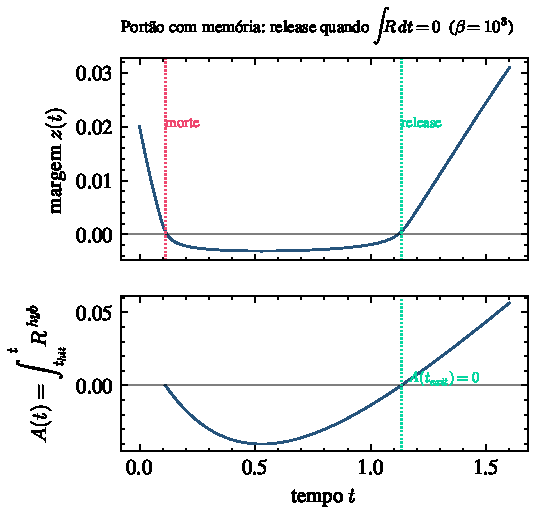
\includegraphics[width=0.72\linewidth]{fig1-mecanismo}
\caption{The memory gate at $\beta=10^3$ (coupled system, reference instance).
Top: the margin $z(t)$ dies at $\thit$, hugs the sticking layer of depth
$\sim\beta^{-1}\log\beta$, and releases. Bottom: the hybrid area
$\Ar(t)=\int_{\thit}^{t}R^{\hyb}$; release coincides with $\Ar=0$ up to
$O(\beta^{-1})$ (\cref{thm:main}). Deterministic Euler integration
($dt=10^{-5}$); the uncertainty is discretization only. Script
\protect\path{t2-prova/figuras_draft.py}.}
\label{fig:mecanismo}
\end{figure}

\subsection{The forcing theorem: the law belongs to the
forcing}\label{sec:forcing}

\Cref{thm:main} is stated for two neurons, and read literally it is a statement
about a particular small network. It is not: nothing in the argument uses the
live side except through the scalar $R$ it generates. This subsection makes that
reading a theorem. The residual becomes a \emph{prescribed forcing}, the live
side becomes an arbitrary affine subsystem of order $m$, and the law, the rate
and the first-order coefficient are unchanged. The complete proof is
\cref{app:forcing}; the mathematical source is the standalone note
\path{06-notas/t2-prova/teorema-forcing-draft.tex}.

\paragraph{Network and live class.} Keep the data and the loss of
\cref{sec:setup}, but allow $m+1$ units with \emph{fixed} readout weights, the
readout of the unit that dies normalized to $+1$:
\begin{equation}\label{eq:netF}
f_\theta(x)=g_\beta(w_0x+b_0)+\sum_{k=1}^{m}a_k\,g_\beta(w_kx+b_k) .
\end{equation}
Unit $k=0$ is the unit $A$ that dies. Only its readout enters $c$ and the margin
equation, so fixing it at $+1$ is a normalization and not a restriction; we
reserve $a_0$ for the floor of the area, as in \cref{app:lemmas}. The
remaining $m$ units form the live subsystem $B$, with parameters
$\theta_B\in\R^{2m}$, and $R$ is the residual excluding $A$, exactly
\eqref{eq:residual} with $f_{-A}=\sum_{k\ge1}a_kg_\beta(w_kx+b_k)$. Write
$\res_i=f_\theta(x_i)-y_i$ and $\Tep=\texit-\thit$ for the length of the
episode.

We call $B$ \emph{affine of order $m$} on a window if, on that window, the
activation pattern of every live unit is constant and the readout is fixed. Then
$f_{-A}$ is linear in $\theta_B$: with $\varphi_i\in\R^{2m}$ the feature vector
of datum $i$, $(\varphi_i)_{2k-1}=a_k\mathbf 1_{k,i}x_i$ and
$(\varphi_i)_{2k}=a_k\mathbf 1_{k,i}$, one has
$f_{-A}(x_i;\theta_B)=\varphi_i\cdot\theta_B$ up to the softplus defect, and the
ReLU $B$-field is $-G_B(\theta_B-\theta_B^\ast)$ with
\begin{equation}\label{eq:gramF}
G_B=\frac1n\sum_{i=1}^n\varphi_i\varphi_i^{\!\top}\in\R^{2m\times2m},
\qquad G_B\succeq0 .
\end{equation}
This is the only structural fact about $B$ used below, and it holds for
\emph{every} $m$: a one-hidden-layer network with frozen activation pattern,
fixed readout and only the first layer trained is linear in its trainable
parameters, and $G_B$ is then a Gram matrix, hence positive semidefinite. We
write $G$ for the full $(2m+2)\times(2m+2)$ Gram of the network with $A$ alive
and pattern frozen, and $G_{BA}$ for its $B\times A$ block; $G$, and hence its
principal submatrix $G_B$, is PSD.

\paragraph{Hypotheses.} All of them are statements about the forcing $R$ and
about the hybrid reference trajectory, both computable by a single ReLU
integration with $A$ frozen. None constrains $m$, the dimension of $\theta_B$,
or the functional form of $f_{-A}$ beyond the affine class.

\begin{itemize}
\item[(H0$'$)\hyplabel{H0$'$}{H0p}] \textbf{Regularity of the forcing.}
$R^{\hyb}\in C^1([\thit,H])$ with $\|\dot R^{\hyb}\|_\infty\le C_R$.
\item[(H1$'$)\hyplabel{H1$'$}{H1p}] \textbf{Transversal entry.} $R^{\hyb}(\thit)<0$; the arrival
speed is $v=c\,|R^{\hyb}(\thit)|>0$.
\item[(H2$'$)\hyplabel{H2$'$}{H2p}] \textbf{Transversal exit at the zero of the area.} $\Ar^{\hyb}$
has a first zero at $\texit<H$, with $R^{\hyb}(\texit)>0$, $\Ar^{\hyb}<0$ on
$(\thit,\texit)$, and, for each $\delta>0$, $|\Ar^{\hyb}|\ge a_0(\delta)>0$ on
$[\thit+\delta,\texit-\delta]$.
\item[(H3$'$)\hyplabel{H3$'$}{H3p}] \textbf{Lipschitz response.} There is $\mathrm{Lip}_R$ with
$|R[\theta_B]-R[\theta_B']|\le\mathrm{Lip}_R\|\theta_B-\theta_B'\|$, and the
$B$-field is Lipschitz on a compact tube around the hybrid trajectory. In the
affine class this is automatic, with $\mathrm{Lip}_R=\|\varphi_j\|$; we keep it
as a hypothesis so that the statement survives outside the class.
\item[(H4$'$)\hyplabel{H4$'$}{H4p}] \textbf{Isolated episode, uniform live margins.} No unit other
than $A$ switches on $[0,H]$, and the live margins are \emph{uniformly} bounded
away from the kink,
\[
\bigl|z_k(x_i;\theta_B(t))\bigr|\ \ge\ \delta_B>0
\qquad\text{for all }k=1,\dots,m,\ i=1,\dots,n,\ t\in[0,H],
\]
along both the hybrid and the $\beta$-trajectory. The other margins of $A$ stay
$\le-\delta_1<0$. Finally, $A$ itself switches \emph{exactly twice} on $[0,H]$,
at $\thit$ and at $\trel$; in particular $z\ge\delta_1'>0$ on $[\trel+\eta,H]$
along both trajectories, for some $\eta,\delta_1'>0$.
\item[(H5$'$)\hyplabel{H5$'$}{H5p}] \textbf{Bounded residuals.} $|\res_i(t)|\le C_{\mathrm{res}}$ for
all $i$ and all $t\in[0,H]$, along both trajectories in the tube.
\end{itemize}

\begin{remark}[\eqref{H4p} is the definition of the window, and why it had to be
reinforced]\label{rem:H4F}
Two things are going on in \eqref{H4p}, and they should not be confused. The
\emph{uniform} margin floor $\delta_B$ is a genuine strengthening of \eqref{H4}
of \cref{sec:setup}: in the two-neuron case the single live unit contributes one
softplus-versus-ReLU discrepancy, absorbed silently into the
$O(e^{-\beta\delta_1})$ bookkeeping; with $m$ live units there are $mn$ such
discrepancies, and a per-instance margin is not enough --- the bound must be
uniform over units, data and time, or the sum of $mn$ terms is not controlled by
a single exponential. The constancy of the pattern, on the other hand, is not a
debt but a \emph{definition of scope}: \cref{thm:forcing} holds on any maximal
window on which the live activation pattern is constant and which contains
$\thit$ and $\texit$, and such a window is identified a posteriori by the same
hybrid integration that checks \eqref{H1p}--\eqref{H2p}. Relaxing it is not free, and
the price is exhibited in \cref{app:forcing-open}: the two flows then switch at
different instants, the difference of drifts acquires a term
$-(G_B-G_B')\theta_B$ that is not of the form $-(\text{PSD})\Delta$, and one is
back to a Gr\"onwall factor $\exp(\sum_k\|\Delta G_k\|\|\theta_B\|/v_k)$ ---
exponential in $m$ in the worst case, which is exactly what the estimate of
\cref{lem:gronwallF} was introduced to remove.
\end{remark}

\begin{theorem}[entry--exit law, forcing form]\label{thm:forcing}
Let $A$ be a softplus-$\beta$ unit with fixed readout $+1$ and margin $z$ on the
face $j$, coupled to a live subsystem $B$ affine of order $m$, and let $R$ be
the residual \eqref{eq:residual} it generates. Assume
\textup{\eqref{H0p}--\eqref{H5p}}. Then there is $\beta_0<\infty$ such that for
$\beta\ge\beta_0$:
\begin{enumerate}
\item[(i)] \emph{(sticking)} on compact subintervals of $(\thit,\texit)$ the
margin satisfies $u=c\beta|\Ar^{\hyb}(t)|(1+o(1))$, that is
$z_{\mathrm{park}}(t)=-\beta^{-1}\log\beta\,(1+o(1))$;
\item[(ii)] \emph{(release)} the first return of $z$ to $0$ after death obeys
\begin{equation}\label{eq:releaseF}
t^\beta_{\mathrm{release}}
=\texit-\frac{1}{c\,R^{\hyb}(\texit)}\cdot\frac1\beta+o(\beta^{-1}),
\end{equation}
where $\texit$ is the first zero of the hybrid area $\Ar^{\hyb}$;
\item[(iii)] \emph{(uniform approximation)} for every $\delta>0$,
\begin{equation}\label{eq:supF}
\sup_{t\in[0,H]\setminus(B_\delta(\thit)\cup B_\delta(\texit))}
\bigl\|\theta^\beta(t)-\theta^\infty(t)\bigr\|
=O_\delta\!\left(\frac{\log\beta}{\beta}\right),
\end{equation}
the $\log\beta$ being carried solely by the normal coordinate of $\theta_A$;
\item[(ivA)] \emph{(live subsystem, up to release)}
\begin{equation}\label{eq:ivA}
\sup_{[0,\trel]}\bigl\|\theta_B^\beta-\theta_B^{\hyb}\bigr\|
\ \le\ 2M_2\frac{\log\beta}{\beta^2};
\end{equation}
\item[(ivB)] \emph{(live subsystem, after release)} against the hybrid limit
$\theta^\infty$ of \cref{def:hybrid}, in which $A$ is alive again,
\begin{equation}\label{eq:ivB}
\sup_{[\trel,H]}\bigl\|\theta_B^\beta-\theta_B^{\infty}\bigr\|
\ \le\ \frac{M_3}{\beta},
\qquad
M_3=H\,\|G_{BA}\|\,C_A+2M_2\frac{\log\beta}{\beta}+\frac{C_fH}{v'} ,
\end{equation}
so that in particular
$\sup_{[0,H]}\|\theta_B^\beta-\theta_B^{\infty}\|=O(\beta^{-1})$: the live
subsystem never carries the $\log\beta$.
\end{enumerate}
Here $v'=cR^{\hyb}(\texit)>0$ is the exit speed, $C_A$ is the constant of
\eqref{eq:postrelA}, and
\begin{equation}\label{eq:M2F}
M_2=\frac{C_fC_4}{c},
\qquad
C_4=\frac{2}{c\min\bigl(|R^{\hyb}(\thit)|,R^{\hyb}(\texit)\bigr)}+\frac{\Tep}{a_0},
\qquad
C_f=\frac{\|\varphi_j\|}{n}.
\end{equation}
\end{theorem}

The word ``in particular'' in (ivB) is legitimate because the two references
agree to the required order where the two clauses are glued:
$\theta^\infty\equiv\theta^{\hyb}$ on $[0,\texit]$ \emph{by definition}
(\cref{def:hybrid}), and on the short interval $[\texit,\trel]$, of length
$O(\beta^{-1})$ by \eqref{eq:releaseF}, they differ only by the drift that $A$'s
revival induces in $\theta^\beta$, itself $O(\beta^{-1})$ because
$z=O(\beta^{-1})$ there; the product is $O(\beta^{-2})$. Hence \eqref{eq:ivA}
may be read against either reference on $[0,\trel]$, which is also what licenses
$\|\Delta(\trel)\|\le 2M_2\log\beta/\beta^2$ as the initial datum of step~5.

\begin{remark}[why item (iv) changes reference at $\trel$]\label{rem:ivrefF}
The two clauses cannot be merged into a single
$\sup_{[0,H]}\|\theta_B^\beta-\theta_B^{\hyb}\|$. The hybrid $\theta^{\hyb}$
keeps $\theta_A$ frozen at $z=0$ \emph{forever}, so after $\texit$ its residuals
never see $A$; the $\beta$-flow, and $\theta^\infty$, do. On $[\trel,H]$ the
$B$-gap against $\theta^{\hyb}$ is therefore $\Theta(1)$, not
$O(\log\beta/\beta^2)$, and a statement of item~(iv) with $\theta^{\hyb}$ over
all of $[0,H]$ would be false. The correct post-release reference is
$\theta^\infty$, and the rate there is $O(\beta^{-1})$ --- one power worse than
during the episode, because the $O(\beta^{-1})$ mismatch of the release
\emph{instant} feeds into $B$ through the cross block $G_{BA}$ over a horizon of
length $H$, but still one $\log\beta$ better than item~(iii). The constant in
\eqref{eq:ivA} is $2M_2$, not $M_2$: $M_2$ is what the improvement step of
\cref{lem:bootstrapF}(4.1) returns ($\tfrac32M_2$ in fact), while $2M_2$ is what
the closed induction propagates.
\end{remark}

\paragraph{What is new, and what it means.} Three things in \cref{thm:forcing}
are new relative to \cref{thm:main}. First, $B$ is any affine subsystem of any
order $m$, not one live neuron. Second, $M_2$ carries \emph{no} factor
$e^{L_BH}$: the Gr\"onwall estimate of \cref{lem:gronwall} is replaced by an
energy estimate that uses only $G_B\succeq0$, which is what removes the only
exponential in $m$ from the constants and, with it, any restriction of the form
$m\cdot H$ small. Third, $C_f\le\|(x_j,1)\|(\sum_ka_k^2)^{1/2}/n$ grows at most
like $\sqrt m$, so every constant in \eqref{eq:M2F} is polynomial in $m$
(\cref{app:forcing-uniform}). The reading is that \emph{the law is a statement
about the forcing, not about whatever generates it}: the first-order
coefficient $-1/(cR^{\hyb}(\texit))$ is built from $c$ and from the hybrid
forcing at one instant, and the cancellation that produces it is arithmetic in
$R$ (\cref{rem:cancelF}), so structurally $m$ cannot appear in it. Any
$m$-dependence must live in the remainder, that is in $\beta_0$ --- and the next
proposition says how much.

\begin{proposition}[polynomial threshold]\label{prop:beta0}
Under \textup{\eqref{H0p}--\eqref{H5p}}, the threshold of \cref{thm:forcing} may be
taken to be $\beta_0=\max(\beta_1,\dots,\beta_5)\lesssim O(m)$ at fixed forcing
--- that is, with $a_0$, $R^{\hyb}(\thit)$, $R^{\hyb}(\texit)$, $\Tep$,
$\delta_B$, $\delta_1$, $C_{\mathrm{res}}$, $X_{\max}=\max_i\|(x_i,1)\|$ and $H$
held fixed while $m$ grows --- with the implied constant a fixed rational expression in
$a_0^{-1}$, $R^{\hyb}(\texit)^{-1}$, $|R^{\hyb}(\thit)|^{-1}$, $\Tep$, $H$,
$X_{\max}$, $C_{\mathrm{res}}$, $\delta_B^{-1}$ and $c$. The five conditions and
the identification of the binding one are \cref{tab:beta0}.
\end{proposition}

In particular $\beta_0$ is polynomial, indeed linear, in the size of the live
subsystem: the theorem is not vacuous for large $m$. What is \emph{not}
controlled is the dependence of $\beta_0$ on the forcing itself, which enters
through $1/a_0$ and $1/R^{\hyb}(\texit)$, and which is exactly what the numerics
of \cref{sec:forcing-numerics} see.

\subsection{The six lemmas}\label{sec:lemmas}

The proof of \cref{thm:main} reduces the episode to a scalar entry--exit problem
through the six lemmas below (their forcing-form counterparts are in
\cref{app:forcing}); they are proved in \cref{app:lemmas}. Each also carries a committed executable symbolic or
numerical verification (\texttt{passo0--6}, \texttt{prova\_L1--L6}), whose
outcome is reported at the end of each proof.

\begin{lemma}[normal form and additive quadrature]\label{lem:gauge}
Let $w=e^{\beta z}$ and $u=1/w$, and set $\Psi(u)=\log u+u$. In fast time
$\tau=\beta t$ the margin obeys
\begin{equation}\label{eq:normalform}
\frac{dw}{d\tau}=c\,R(t)\,\frac{w^{2}}{1+w}\,(1+E_\beta),
\qquad
|E_\beta|\le\frac{\log(1+w)}{\beta|R|},
\end{equation}
the quadratic normal form of De Maesschalck and
Schecter~\cite[equations~(1.9)--(1.10)]{DMS16} with $\varepsilon=\beta^{-1}$,
and one has the exact additive
identity
\begin{equation}\label{eq:quadrature}
\frac{d\Psi(u)}{dt}=-c\,\beta\,R(t)+c\log(1+w)+\mathcal{E}_{\eqref{H3}}(t),
\qquad
\bigl|\mathcal{E}_{\eqref{H3}}\bigr|\le C_3\,\beta\,e^{-\beta\delta_1}.
\end{equation}
Under \eqref{H1}--\eqref{H2} the additive correction satisfies
$\int_{\thit}^{\trel}c\log(1+w)\,ds=O(\log\beta/\beta)$.
\end{lemma}

\noindent The bound $|E_\beta|\le\log(1+w)/(\beta|R|)$ in
\eqref{eq:normalform} degenerates at the interior zero of $R$ that
\eqref{H1}--\eqref{H2} force, since $R$ changes sign inside the episode; that
is precisely why the proof switches to the quadrature $\Psi$ of
\eqref{eq:quadrature}, which never divides by $R$.

\begin{lemma}[$B$-subsystem and feedback]\label{lem:gronwall}
Under \eqref{H4} the $B$-field is affine with Lipschitz constant
$L_B=\lambda_{\max}(G_B)$, where $G_B$ is the Gram matrix of the active data, and
$R^{\hyb}$ is affine in $\theta_B$. Integral Gr\"onwall consuming the bound of
\cref{lem:gauge} gives, conditionally on the layer being maintained (supplied by
\cref{lem:bootstrap}),
\begin{equation}\label{eq:Brate}
\sup\bigl\|\theta_B^\beta-\theta_B^{\hyb}\bigr\|=O\!\left(\frac{\log\beta}{\beta^{2}}\right),
\end{equation}
one full order better than the naive $O(\beta^{-1})$: in the bulk
$u=O(\beta|\Ar|)$, so the coupling is $O(\beta^{-2})$ there and $O(\beta^{-1})$
only in the $O(\beta^{-1})$-wide corner windows.
\end{lemma}

\begin{lemma}[entry corner]\label{lem:corner-in}
Let $v=c\,|R^{\hyb}(\thit)|$ be the arrival speed, transversal by \eqref{H1}. The
exact identity $(1-\sigma(s))/\sigma(s)=e^{-s}$ collapses the crossing-time
difference to an elementary integral and gives
\begin{equation}\label{eq:corner-in}
t_{\mathrm{cross}}^{\beta}=\thit+\frac{1}{\beta v}\bigl(1+O(\delta_z)+o(1)\bigr),
\qquad
\bigl\|\theta^\beta(t_{\mathrm{cross}})-\theta^\infty(\thit)\bigr\|=O(\beta^{-1}),
\end{equation}
where $t^\beta_{\mathrm{cross}}$ is the first time with $w=w_0$. The
exponentially weighted approach integral is $\tfrac{3/2}{\beta v}(1+o(1))$, the
factor $3/2$ coming from $\int_0^\infty e^{-s}(1+e^{-s})\,ds$.
\end{lemma}

\begin{lemma}[sticking and release for prescribed $R$]\label{lem:release}
Let $R\in C^1$ be prescribed and satisfy \eqref{H1}--\eqref{H2}, and write
$\Ar(t)=\int_{\thit}^{t}R$. Then

(i) $\Psi(u(t))=\Psi(u_0)-c\beta\Ar(t)+\mathrm{corr}(t)$ with
$0\le\mathrm{corr}(t)=\int c\log(1+w)\,ds=O(\log\beta/\beta)$; on compact
subintervals of $(\thit,\texit)$,
$u=c\beta|\Ar(t)|\bigl(1+O(\log\beta/(\beta a_0))\bigr)$, so the sticking depth is
$z\sim-\beta^{-1}\log\beta$;

(ii) the release obeys the closed formula
\begin{equation}\label{eq:release-prescribed}
\trel-\texit=\frac{\mathrm{corr}(\beta)}{c\,\beta\,R(\texit)}\,(1+o(1))
=O\!\left(\frac{\log\beta}{\beta^{2}}\right),
\end{equation}
so $u$ returns to $O(1)$ at $\texit+O(\beta^{-1})$, with no $\log\beta$ factor;

(iii) a perturbation $\tilde R=R+\delta$ shifts $\texit$ by at most
$\delta\,(\texit-\thit)/R(\texit)+O(\delta^{2})$.

No division by $R$ occurs anywhere: the layer is held by the area, not by the
sign of $R$, and the interior zero of $R$ forced by \eqref{H1}--\eqref{H2} is
harmless.
\end{lemma}

\begin{lemma}[coupled bootstrap]\label{lem:bootstrap}
Under \eqref{H1}--\eqref{H4} the coupled system satisfies the two-term law
\begin{equation}\label{eq:twoterm}
t^\beta_{\mathrm{release}}
=\texit-\frac{1}{c\,R^{\hyb}(\texit)}\cdot\frac{1}{\beta}
+\frac{\mathrm{corr}(\beta)}{c\,\beta\,R^{\hyb}(\texit)}+o(\beta^{-1}),
\qquad \mathrm{corr}(\beta)=O\!\left(\frac{\log\beta}{\beta}\right),
\end{equation}
obtained by continuation with strict margins, with the constant
$M_2=e^{L_BH}C_fC_4/c$ independent of the continuation hypothesis for
$\beta\ge\beta_0$. In the first-order coefficient the arrival speed cancels: in
the product $K\,|R^{\hyb}(\thit)|/R^{\hyb}(\texit)$ of the entry delay by the
area it cuts, the factor $|R^{\hyb}(\thit)|$ cancels against
$K=1/(c|R^{\hyb}(\thit)|)$ of \cref{lem:corner-in}, leaving a coefficient that
still depends on $c$ and on $R^{\hyb}(\texit)$.
\end{lemma}

\begin{lemma}[exit corner, branch selection and scalar reduction]\label{lem:corner-out}
Under \eqref{H1}--\eqref{H4}, after release: (i) the $\beta$-trajectory crosses
the exit corner in time $\tfrac{1}{\beta v'}(1+o(1))$ with
$v'=c\,R^{\hyb}(\texit)>0$, the mirror of \cref{lem:corner-in}; (ii) the ReLU flow
restarted at $(\theta_A(\thit),\theta_B^{\hyb}(\texit))$ has forward uniqueness on
the activating branch, and that branch is selected by the limit itself, the
frozen Filippov branch~\cite{Fil88} being incompatible with release at
$\texit+O(\beta^{-1})$; (iii) classical Gr\"onwall glues on $[\trel,H]$ at rate
$O(\log\beta/\beta)$. Under \eqref{H3} the other data contribute
$O(e^{-\beta\delta_1})$, the face-$j$ field is rank one along $(x_j,1)$, and the
episode reduces to the scalar problem.
\end{lemma}

\subsection{Proof of the theorem}\label{sec:proofmain}

\begin{proof}[Proof of \cref{thm:main}]
We compose the six lemmas along the four stages of the episode.

By \cref{lem:corner-out} the field on $\theta_A$ splits under \eqref{H3} into a
rank-one part along $(x_j,1)$ and terms of size $O(e^{-\beta\delta_1})$, so the
tangential components of $\theta_A$ are frozen at an exponential rate and the
normal component is exactly the scalar problem of
\crefrange{lem:gauge}{lem:bootstrap}.

On $[0,\thit-\delta]$ both flows are the ReLU flow up to the softplus defect,
which is bounded by $C e^{-\beta z^0(t)}$; step~1 of the proof of
\cref{lem:corner-in} integrates that defect against the trajectory and gives a
gap $O(\beta^{-1})$. \Cref{lem:corner-in} then delivers the entry corner: the
crossing time is $\thit+1/(\beta v)(1+o(1))$ and the state at crossing is
$O(\beta^{-1})$ from $\theta^\infty(\thit)$.

On $[\thit+\delta,\texit-\delta]$, \cref{lem:bootstrap} closes the feedback loop:
its continuation argument keeps the margin strictly inside the layer and
$\theta_B$ within $O(\log\beta/\beta^{2})$ of the hybrid, by consuming
\cref{lem:gronwall} (which needs the layer) and \cref{lem:release}(iii) (which
tolerates the resulting perturbation of the forcing). Inside the layer
\cref{lem:release}(i) gives the depth $z\sim-\beta^{-1}\log\beta$, and this is the
largest of the three contributions to \eqref{eq:sup}; $\theta_B$ contributes
$O(\log\beta/\beta^{2})$ and the tangential part of $\theta_A$ contributes
$O(e^{-\beta\delta_1})$. Hence the supremum over this stage is
$O_\delta(\log\beta/\beta)$, carried by the normal coordinate alone, which proves
the sharpness asserted in \cref{rem:mechanism}.

The terminal window and the release law are \cref{lem:bootstrap} step~5: the
correction delay of \cref{lem:release}(ii) is $O(\log\beta/\beta^{2})$, the
perturbation of the forcing shifts $\texit$ by $O(\log\beta/\beta^{2})$ by
\cref{lem:release}(iii), and the area cut by the entry corner advances the exit by
$-1/(cR^{\hyb}(\texit)\beta)$. Summing the three gives \eqref{eq:twoterm}, hence
\eqref{eq:release}.

Finally \cref{lem:corner-out} crosses the exit corner in time $O(\beta^{-1})$,
selects the activating branch, and glues the two flows on $[\trel,H]$ at rate
$O(\log\beta/\beta)$. Taking the maximum of the four stage bounds gives
\eqref{eq:sup}.
\end{proof}

\begin{figure}[t]
\centering
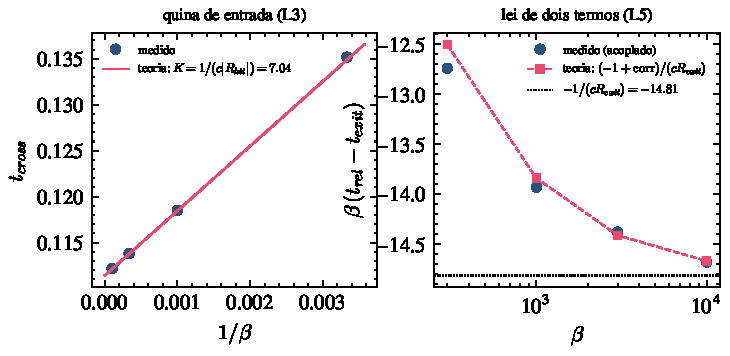
\includegraphics[width=0.88\linewidth]{fig2-constantes}
\caption{Predicted constants against measurements (deterministic runs; the
uncertainty is discretization). Left: entry-corner crossing times against
$1/\beta$; the line is the proved slope
$K=1/(c|R^{\hyb}(\thit)|)=7.04$ (\cref{lem:corner-in}), not a fit. Right: the
two-term release law (\cref{lem:bootstrap}, squares) against the coupled
measurements (circles) over $\beta\in[3\cdot10^2,10^4]$; the dotted line is the
speed-independent first-order coefficient
$-1/(cR^{\hyb}(\texit))=-14.81$. Every coupled
run uses the explicit Euler step $dt=\min(10^{-5},0.02/\beta)$, so
$dt=10^{-5}$ at $\beta=3\cdot10^{2}$ and $10^{3}$, $6.7\cdot10^{-6}$ at
$3\cdot10^{3}$ and $2\cdot10^{-6}$ at $10^{4}$; \cref{tab:dt} refines that step at
$\beta=10^{4}$. Script \protect\path{t2-prova/figuras_draft.py}.}
\label{fig:constantes}
\end{figure}

\subsection{Numerical verification on one instance}\label{sec:numerics}

The reference instance is $X=(0.5,1.5)$, $Y=(0.5,1.0)$,
$\theta_A(0)=(-0.5,0.27)$, $\theta_B(0)=(1.144,0.261)$, giving $\thit=0.1114$,
$\texit=1.1325$ and $\delta_1=0.508$. Every empirically measured constant is
predicted by the proofs: the entry coefficient is $K_{\mathrm{teo}}=7.04$ against
$7.13$ fitted ($1.2\%$); the coupled two-term law
$(-1+\mathrm{corr})/(cR_{\mathrm{exit}})$ reproduces the fine-grid coupled sweep
$-12.74/-13.93/-14.38/-14.68$ to $1.9\%/0.7\%/0.2\%/0.1\%$ for
$\beta=3\cdot10^2\ldots10^4$, with the coefficient
$1/(cR_{\mathrm{exit}})=14.815$ that the cancellation leaves (against
$-14.68$ the leading coefficient alone
is at $0.9\%$); the tangential drift is at machine zero. This subsection is one
instance; \cref{sec:sweep} tests the same law on a sweep of drawn instances.

The measured coefficient is a discretization, not a fit, so it must be shown to
converge. \Cref{tab:dt} is that test: it refines the Euler step at the stiffest
point of the sweep, $\beta=10^{4}$, keeping everything else fixed, and asks
whether the measured offset approaches the \emph{proved} limit $-14.815$ of
\eqref{eq:twoterm} rather than some nearby number.

\begin{table}[t]
\centering
\caption{A convergence test for the two-term law, not a table of measurements:
the proved coefficient $-1/(cR^{\hyb}(\texit))=-14.815$ is the limit, and the
rows are successive refinements of the Euler step at $\beta=10^{4}$ that must
approach it. They do, monotonically, closing to $0.1\%$ at the finest step; a law
with the wrong constant would leave a floor here instead. The
correction term of \cref{lem:bootstrap} is $\mathrm{corr}=0.00977$ at every step,
so what is refining is the quadrature and not the law. At $dt=10^{-5}$ the
measurement is quantized in units of $\beta\,dt=0.1$, which is the whole of that
row's error. The sweep of \cref{sec:numerics} and \cref{fig:constantes} uses
$dt=\min(10^{-5},0.02/\beta)$, that is $dt=2\cdot10^{-6}$ at $\beta=10^{4}$.}
\label{tab:dt}
\begin{tabular}{@{}lrr@{}}
\toprule
$dt$ & $\beta(\trel-\texit)$ & deviation from $-14.815$ \\
\midrule
$10^{-5}$          & $-14.000$ & $5.5\%$ \\
$2\cdot10^{-6}$    & $-14.680$ & $0.9\%$ \\
$10^{-6}$          & $-14.760$ & $0.4\%$ \\
$5\cdot10^{-7}$    & $-14.805$ & $0.1\%$ \\
\bottomrule
\end{tabular}
\end{table}

\noindent It converges to the proved coefficient: $0.1\%$ at the finest step.
The driver reuses \path{roda_acoplado} verbatim from
\path{t2-prova/prova_L5_verificacao.py}, overriding only the step.

\subsection{From one instance to a law}\label{sec:sweep}

A single instance cannot distinguish a law from a coincidence of constants, so
we ran the same test over drawn instances. The script \path{sweep_instancias.py}
samples 600 triples $(X,Y,\theta(0))$ from a prior fixed in advance and
documented in the script, integrates each with the same $dt$, the same
integrator and the same $\beta=10^{4}$ as the canonical run --- the coupled
driver is copied verbatim from \path{passo4_verificacao.py} --- and compares the
measured release offset $\beta(\trel-\texit)$ against the prediction
$-1/(c\,R^{\hyb}(\texit))$ formed from that instance's own constants. As a
sanity check the reference instance of \cref{sec:numerics} is reproduced inside
the sweep, at $2.9\%$.

Of the 600 draws, 57 satisfy \eqref{H1}--\eqref{H4}. The exclusions are
accounted for exactly: 340 have no death within the horizon, 162 fail
\eqref{H2} because the area never returns to zero, and 41 die outside the
detector's window. On the 57 admissible instances the resurrection occurs in
$57/57$ --- the release always precedes the hybrid $\texit$ --- and the relative
error of the release coefficient against the instance's own
$-1/(c\,R^{\hyb}(\texit))$ has median $2.68\%$, ninetieth percentile $7.26\%$
and maximum $12.01\%$. The predicted coefficients themselves range over
$[-91.8,-4.5]$, a factor of 20, so the agreement is not the agreement of one
number repeated. The worst quartile, those with $|{\rm predicted}|$ between
$4.5$ and $7.1$, has median error $6.7\%$.

Two caveats belong with those numbers. First, the residual error is not
centred: the median ratio of measured to predicted is $0.975$ and $55$ of the
$57$ instances have $|{\rm measured}|<|{\rm predicted}|$. That systematic
shortfall is the $o(\beta^{-1})$ remainder of \cref{thm:main} at a finite
$\beta$, not sampling noise, and it is reported as a bias rather than absorbed
into a tolerance. Second, the fraction $57/600$ is a property of the prior and
measures nothing about how large the set \eqref{H1}--\eqref{H2} is. The
geometric number is the conditional one: of the 219 deaths that fall inside the
detector's window, 57, that is $26\%$, satisfy \eqref{H2}. The memory gate is a
real and restrictive condition, not a formality that a generic trajectory
satisfies.

\subsection{Verification of the forcing theorem}\label{sec:forcing-numerics}

The sweep above tests \cref{thm:main} on two-neuron instances. \Cref{thm:forcing}
claims something the sweep cannot see, namely that the number of live units does
nothing, so it needs its own campaigns. Five were run, in
\path{05-experimentos/t2-n-neuronios/} (scripts \path{verifica_forcing.py},
\path{parecer14.py} and \path{beta.py}, the fifth being the pre-hit campaign
whose own scripts are named with it below); none of them is part of the proof,
and we say what each does and does not establish.

\emph{(1) The $m$-sweep with NTK readout.} Sixty-six instances pass
\eqref{H1p}--\eqref{H4p} --- $23$ at $m=4$, $21$ at $m=8$, $22$ at $m=16$ --- against a
$57$-instance two-neuron baseline, at $\beta=10^4$, explicit Euler with
$dt_0=10^{-5}$ on the hybrid and $dt=2\cdot10^{-6}$ on the coupled flow,
$H=1.8$ (the campaign horizon, distinct from the $H=1.7$ of the reference
instance). No free parameter is fitted: the predicted coefficients span
$[-109,-14]$, a factor of $7.6$, the measured ones $[-132,-14]$, with
$R^2=0.950$ against the unfitted law, and an OLS slope of $1.154$
($R^2=0.968$). Median relative errors are
$0.80\%/6.85\%/5.58\%$ at $m=4/8/16$, against $2.68\%$ for the baseline. In an
OLS of the error on $(\log_2m,\ 1/R^{\hyb}(\texit),\ \Tep)$ the coefficient of
$\log_2m$ is not significant ($t=0.71$) while $1/R^{\hyb}(\texit)$ is
($t=2.56$); in the joint regression over both readout families ($n=133$, over
which $\lambda_{\max}(G_B)$ ranges from $1.4$ to $56.1$, so that $e^{L_BH}$
would vary by $42$ orders of magnitude) only $1/R^{\hyb}(\texit)$ is significant
($t=7.44$), with $\log_2m$ at $t=-0.09$ and $\log\lambda_{\max}$ at $t=-0.47$.
This is consistent with the remainder being governed by exit transversality
rather than by $m$; it is not conclusive.

\emph{(2) Bit-identical cloning} ($23$ instances). Each accepted $m=4$ instance
is replayed with every live unit split into $p$ copies carrying readout
$a_k/\sqrt p$ and parameters $(w_k,b_k)/\sqrt p$, so that $f_B$, the NTK and the
whole flow --- hence $R(t)$ --- are unchanged while $m\to pm$. The measured
errors are identical to machine precision at $m=4,8,16$ (median $0.80\%$,
maximum $16.17\%$ in all three columns), and $\lambda_{\max}(G_B)$ is likewise
invariant. This isolates the claim that at fixed forcing the number of live
units does nothing, and it is the closest numerical analogue of
\cref{rem:cancelF}.

\emph{(3) The unit-readout family} ($67$ instances: $22/24/21$ at $m=4/8/16$,
median error $1.16\%/4.52\%/5.35\%$, maximum $\approx28\%$ at $m=8,16$ and
$\approx20\%$ at $m=4$). Here
$\lambda_{\max}(G_B)$ grows with $m$ and the published constant
$e^{L_BH}C_fC_4/c$ would be exponential. The law survives, with the same
qualitative degradation pattern; under the PSD constant \eqref{eq:M2F} this is
expected, under $e^{L_BH}C_fC_4/c$ it would not be. Across the joint sample
$\lambda_{\max}(G_B)$ spans $1.4$ to $56.1$, so $e^{L_BH}$ varies by $42$
orders of magnitude while the measured error is flat in it ($t=-0.47$) and
tracks only $1/R^{\hyb}(\texit)$ ($t=7.44$): no estimate carrying that factor
can be the operative one. This is the empirical case for \cref{lem:gronwallF}
being the right estimate.

\emph{(4) The $\beta$ sweep on the worst instances.} The six worst $m=8$
instances of item~(1), with errors $11.9$--$20.5\%$ at $\beta=10^4$, were rerun
at $\beta=3\cdot10^4$ with the same integrator and the same predicted
coefficients, which are properties of the hybrid reference and therefore
unchanged. The errors collapse to
$20.45\to0.35$, $20.20\to4.93$, $17.30\to0.20$, $13.52\to4.23$,
$12.62\to0.30$, $11.88\to0.50$ (per cent), on every instance. This is the
sharpest available evidence that the $m=8,16$ degradation of item~(1) is a
$\beta_0$ effect --- the asymptotic regime bites later --- and not a failure of
the law.

\paragraph{The two exponents of the pre-hit gap, measured.} Step~4 of
\cref{lem:gronwallF} predicts two \emph{different} rates at the hit:
$\rho_A(\thit)=O(\beta^{-1})$, because the $A$-block of the defect is a
derivative defect and carries no $\beta^{-1}$, and $\rho_B(\thit)=O(\beta^{-2})$,
because the $B$-block sees only $A$'s \emph{output} defect, which does carry a
$\beta^{-1}$. The one-power separation is the whole content of the step and is
falsifiable directly. Twelve instances ($4$ at each of $m=4,8,16$, drawn from
the accepted set of item~(1)) were integrated from $t=0$ to $\thit$ twice, once
with the ReLU field and once with the softplus field, with an RK4 stepper at
$dt=2\cdot10^{-6}$ so that the integration error sits well below $\beta^{-2}$
(scripts \path{parecer15_o5.py}, \path{parecer15_o5b.py}). Sweeping
$\beta\in\{10^3,2\cdot10^3,4\cdot10^3,8\cdot10^3\}$, both compensated quantities
\emph{saturate}, which is the signature of the exponent being exactly right:
$\beta\rho_A$ rises to a plateau near $0.53$ (for instance
$0.404\to0.501\to0.526\to0.528$ on one $m=4$ instance and
$0.426\to0.510\to0.529\to0.530$ on one $m=8$ instance), and $\beta^2\rho_B$
likewise flattens. Instances with small $\beta\thit v$ saturate later, as they
must: the estimate is asymptotic in the number of $e$-foldings available before
the hit. The constant is predicted to be governed by the arrival speed
$v=c|R^{\hyb}(\thit)|$ and \emph{not} by $m$; \cref{tab:o5} is that
prediction measured.

\begin{table}[t]
\centering
\caption{The pre-hit $B$-gap at $\beta=8\cdot10^3$, compensated by the exponent
and the arrival speed that step~4 of \cref{lem:gronwallF} predicts. Over the
twelve instances $\beta^2v\,\rho_B=0.198\pm0.046$, with no trend in $m$: the
$m=4$ mean is the largest and the $m=8$ mean the smallest. What sets the
constant is the transversality of the entry, not the size of the live
subsystem. Scripts \protect\path{parecer15_o5.py},
\protect\path{parecer15_o5b.py}.}
\label{tab:o5}
\begin{tabular}{@{}lccccr@{}}
\toprule
& \multicolumn{4}{c}{$\beta^2 v\,\rho_B(\thit)$, per instance} & mean\\
\midrule
$m=4$  & $0.202$ & $0.253$ & $0.249$ & $0.274$ & $0.244$\\
$m=8$  & $0.203$ & $0.176$ & $0.175$ & $0.119$ & $0.168$\\
$m=16$ & $0.135$ & $0.206$ & $0.212$ & $0.169$ & $0.180$\\
\bottomrule
\end{tabular}
\end{table}

\paragraph{The gap between the numerics and the theorem.} In every instance
generated by these designs, $R^{\hyb}$ changes sign \emph{once} inside the
episode, because the acceptance filter selects a single entry--exit episode with
$\Ar^{\hyb}<0$ throughout. \Cref{lem:releaseF} imposes no such restriction:
\eqref{H2p} constrains the zeros of the \emph{area}, not of $R$, so the theorem
covers forcings that oscillate arbitrarily often inside the episode and the
numerics do not test that regime --- the numerical filter is strictly stronger
than the hypothesis. Conversely, the acceptance rate of \eqref{H1p}--\eqref{H2p} is about $3\%$ of
random initializations in the NTK-readout family and about $20\%$ ($179/900$)
in the unit-readout family, so the hypotheses are
verifiable a posteriori by one hybrid integration but are not guaranteed a
priori by any initialization criterion we know. Finally, the filter of
\path{verifica_forcing.py} rejects any instance in which $A$ dies more than
once, so the last clause of \eqref{H4p} is not merely verifiable in principle: it is
the condition the experiments were already screening on.

\subsection{Independence of the smoothing}\label{sec:regularization}

The release criterion depends only on $\int R\,dt=0$ and not on the sigmoid. For
the erf class, $g_\beta'=\mathcal N(\beta z)$, the coupled system releases at the
same $\texit$ with an $O(\beta^{-1})$ gap; this is verified numerically and not
proved. GELU itself, $z\,\mathcal N(z)$, has a non-monotone derivative and is not
a member of the family for any $\beta$; \cref{sec:transformer-gelu} shows that
this is a distinct mechanism rather than a technicality.

\section{Non-commutation and the plasticity bridge}\label{sec:noncomm}

\Cref{thm:main} is the flow-first limit: one takes $\beta\to\infty$ of
trajectories. The field-first order instead flows the pointwise-limit generalized
gradient, and it freezes degenerate neurons forever. That branch is the rigorous
one of Eberle, Jentzen, Riekert and Weiss~\cite[Theorem 3.3]{EJRW23}, whose
selected solution is unique and has a degenerate set that is non-decreasing in
time; their degenerate stratum is the fully-zero one rather than our functionally
dead neuron, but the convention $\mathrm{ReLU}'(0)=0$ and the no-revival
mechanism are the same.

\begin{proposition}[the two limit orders do not commute]\label{prop:noncomm}
Let $L_\infty$ be the loss of the hard-ReLU network and let $\nabla^0L_\infty$ be
its pointwise-limit gradient, with the convention $\mathrm{ReLU}'(0)=0$; let
$\theta^{\mathrm{FF}}$ solve $\dot\theta=-\nabla^0L_\infty(\theta)$ from
$\theta^{\hyb}(\thit)$, which exists and is unique
by~\cite[Theorem 3.3]{EJRW23}. Assume \eqref{H1}--\eqref{H4}. Then
$\theta_A^{\mathrm{FF}}\equiv\theta_A(\thit)$ on $[\thit,H]$, whereas
$\theta^\infty$ of \cref{def:hybrid} releases $A$ at $\texit<H$. The two limits
therefore disagree on $(\texit,H]$.
\end{proposition}

\begin{proof}
The $A$-block of $\nabla^0L_\infty$ at $\theta$ is
$-\tfrac1n\sum_i\mathrm{res}_i\,\mathbf 1_{\{z_{A,i}>0\}}(x_i,1)$, which vanishes
identically whenever every margin of $A$ satisfies $z_{A,i}\le0$. At $\thit$ the
margin on datum $j$ is zero and, by \eqref{H3}, the remaining margins are
$\le-\delta_1<0$, so the $A$-block vanishes and $\dot\theta_A^{\mathrm{FF}}=0$.
The margins of $A$ are functions of $\theta_A$ alone, so the condition
$z_{A,i}\le0$ for all $i$ is preserved as long as $\theta_A$ is constant, and the
set of such $\theta$ is therefore forward invariant: $\theta_A^{\mathrm{FF}}$
stays at $\theta_A(\thit)$ on all of $[\thit,H]$. By \cref{def:hybrid} and
\eqref{H2}, $\theta^\infty$ restarts the active flow at $\texit<H$ with
$\dot z(\texit^+)=cR^{\hyb}(\texit)>0$, so $z>0$ immediately after $\texit$.
\end{proof}

\begin{corollary}[the bridge to an MLP of the affine class]\label{cor:mlp}
Let a one-hidden-layer network with $m+1$ units, \emph{fixed} readout and a
one-dimensional input be trained by gradient flow on $[0,H]$, and let $A$ be one
of its units. Suppose that on a window $W\subseteq[0,H]$ containing the death
and the return of $A$ the live activation pattern is constant with margin floor
$\delta_B$, that the other margins of $A$ stay $\le-\delta_1<0$, that $A$
switches exactly twice on $[0,H]$, and that the hybrid
reference computed with $\theta_A$ frozen satisfies \eqref{H1p}--\eqref{H2p} and
\eqref{H0p}, \eqref{H5p}. Then \cref{thm:forcing} applies verbatim: for
$\beta\ge\beta_0=O(m)$ the unit is released at
$\texit-1/(c\beta R^{\hyb}(\texit))+o(\beta^{-1})$, where $\texit$ is the first
zero of the area of the residual excluding $A$.
\end{corollary}

\begin{proof}
The hypotheses of the proposition are \eqref{H0p}--\eqref{H5p} with \eqref{H4p} read as the
definition of the window (\cref{rem:H4F}), and a one-hidden-layer network with
fixed readout, constant live pattern and only the first layer trained is affine
of order $m$ in the sense of \cref{sec:forcing}, with $G_B$ the Gram
\eqref{eq:gramF}. Apply \cref{thm:forcing}.
\end{proof}

The content of \cref{cor:mlp} is that it is not an analogy. Without
\cref{thm:forcing} the passage from the theorem to the MLP measurements of
\cref{sec:experiments} could only be declared empirical without qualification;
with it, the passage splits into the three levels (P1)--(P3) of
\cref{sec:intro}. For an MLP of the affine class --- readout held fixed --- the
law is deduced, conditionally on hypotheses that are checked a posteriori by one
hybrid integration and not assumed: \eqref{H1p}--\eqref{H2p} on the hybrid trajectory
and the window of \eqref{H4p}. What remains empirical is precise, and it is the part
that carries the measurements actually reported here: the readout $v_k$ is
trainable in every experiment of \cref{sec:experiments}, which takes the live
field outside the class in which $-G_B\Delta$ is an identity --- this is the
open case of the trainable readout, (O6) of \cref{app:forcing-open}, where an
$e^{L_B\Tep}$ factor, with the episode length rather than the horizon, is
expected to return; several data are active at once; and
the transformer of \cref{sec:transformer} is a different architecture
altogether. We do not claim the corollary covers any number reported in
\cref{sec:experiments}. It covers the object those numbers are evidence about.

Returning to the non-commutation itself: in machine-learning terms it is the
statement behind an empirical trend. Discrete ReLU units that die stay dead --- an exact statement
about a unit's \emph{own} channel under a fixed input, which is the setting of
\cref{prop:noncomm} --- and this is the setting in which the dormant-neuron and
loss-of-plasticity phenomena are usually read~\cite{Sokar23,Lyle23,Dohare24},
mitigated in practice by recycling dead units or by migrating to smooth
activations; the smoothed flow resurrects them by the area law. The channel that
reopens a smoothed unit is $e^{\beta z}$, which closes as $\beta\to\infty$.
\Cref{sec:confirmatory} measures the resulting staircase directly. The
qualification matters: once the input of the layer is itself moving, terminality
is no longer implied, and in our transformer data $20\%$ of injected hard-ReLU
units return ($20/100$ against $0/100$ with the upstream block frozen);
\cref{sec:transformer-gelu} isolates that second channel.

\section{Related work}\label{sec:related}

\paragraph{Entry--exit and geometric singular perturbation.}
The release criterion $\int R\,dt=0$ is the classical entry--exit function of
slow--fast systems~\cite[Theorem 1.1]{DMS16}, applied for instance to a
neurotransmitter release model in~\cite{SDR23}, and \cref{lem:gauge} places our
episode in the quadratic normal form of~\cite[equations~(1.9)--(1.10)]{DMS16} with
$\varepsilon=\beta^{-1}$. Our switching face is degenerate in a way that
literature does not cover: it carries an identically zero field on the dead side.
Generic piecewise-smooth exit theory~\cite{Jef16,GH15,GH22} assumes a nonzero
one-sided field, and the canonical Sotomayor--Teixeira
regularization~\cite{ST98,LST07} requires both one-sided normal components to be
nonzero. The degeneracy is of the exponentially flat type treated by
Kristiansen~\cite{Kri17} with the blow-up method of Krupa and
Szmolyan~\cite{KS01}, but there the forcing is autonomous, whereas here the
residual is generated by the very trajectory it gates. We are not aware of an
analogue of that coupling in the entry--exit literature.

\paragraph{Gradient flows of ReLU networks.} Existence, uniqueness and
convergence rates for gradient flows of ReLU networks are established
in~\cite{EJRW23}, whose selected solution is the field-first branch of
\cref{prop:noncomm}: once a neuron is degenerate it stays degenerate. Our
result is the complementary, flow-first, selection, and the two disagree. The
branch is fixed in practice by a convention of the differentiator, and that
convention has a name: in the framework of Bolte and Pauwels~\cite{BP21} the
derivative returned by automatic differentiation is a definable selection of a
conservative field for the loss, and $\mathrm{ReLU}'(0)=0$ is one such
selection. Their Remark~13 also shows that the nondifferentiability locus
$z=0$ is reached with nonzero probability, so which branch the implementation
picks is not a detail of measure zero: it is the choice that
\cref{prop:noncomm} shows the two limits disagree about.

\paragraph{Dormant neurons and loss of plasticity.} Dead or dormant units are
a measured pathology of trained networks: the dormant neuron phenomenon in
deep reinforcement learning~\cite{Sokar23}, the loss of plasticity under
distribution shift~\cite{Lyle23}, and its persistence in deep continual
learning~\cite{Dohare24}. Death at initialization is a separate and better
understood matter: Lu, Shin, Su and Karniadakis~\cite{Lu20} prove born-dead
results for ReLU networks at initialization and study the initializations that
avoid them. We invoke them only for that regime; every confirmatory count in
this paper conditions on \emph{dynamical} deaths, units that die during
training, and born-dead units are excluded by the instrument. The practical
mitigations are recycling dead units and smoothing the activation.
\Cref{thm:main} and \cref{prop:noncomm} say what the second mitigation buys: a
channel of width $e^{\beta z}$ and a return time set by an area.

\paragraph{Dormancy is not death.} The two objects should not be conflated.
Dormancy in~\cite{Sokar23} is a normalized activation score falling below a
threshold: a unit can be dormant and still have a nonzero column in $J$. Our
object is the exact stratum on which the unit's column of $J$ is identically zero
on every datum. The sets are different, and the apparent tension with deep
reinforcement learning --- whose input is non-stationary by construction, and
where dormancy nonetheless persists --- dissolves once they are kept apart: a
low-score unit need not be on the stratum, so nothing in this paper predicts
that it must return. Our results separate two independent channels. The
\emph{own} channel requires smoothness of the activation, and its width is the
factor $e^{\beta z}$, which the staircase of \cref{fig:escada} measures arm by
arm; for hard ReLU that width is exactly zero. The \emph{upstream} channel
requires only that the layer's input move, and it operates for every activation
we tested, hard ReLU included.

\section{Experiments}\label{sec:experiments}

The claims are tested by prediction, each with its null control, and the failed
designs are reported alongside the successful ones. Every confirmatory analysis
was frozen by a pre-registration commit before the run, and hypotheses that fell
were archived rather than rewritten. The four instruments that carry these claims are
stated as pseudocode in \cref{app:algorithms}. The commits are: pressure pilot
\texttt{b48b527}; rate pilot \texttt{995a87c}; 4a.3 pre-registration
\texttt{a8f8f8c}; 4a.3 confirmatory \texttt{5a961cb}; transformer
pre-registration \texttt{1b45498}.

\paragraph{Statistics.}
Proportions are reported as a point estimate with a two-sided $95\%$
Clopper--Pearson interval~\cite{CP34}; the variability captured is the Bernoulli
count of returns among deaths within a single arm, with the denominator given in
each cell. Event rates $\lambda$, dynamical deaths per run, are reported with a
$95\%$ percentile bootstrap interval over $B=2\cdot10^{4}$ resamples clustered by
seed, so that the variability captured is seed-to-seed and not
episode-to-episode. Nothing is pooled across arms. We write $T$ for the SGLD
temperature, that is, the scale of the injected noise; $T=0$ is deterministic
gradient descent, and $H$ remains the training horizon in optimizer steps.

\subsection{The deterministic schedule is falsified under SGLD}\label{sec:falsification}

Before any confirmatory claim we tested whether the deterministic entry--exit
schedule survives noise. A reduced ``race'' model, pre-registered at commit
\texttt{190d94a} after two adversarial-review rounds, predicts the capture
(resurrection) probability of a dead unit from the mean residual schedule; the
falsifying run of 2700 runs under SGLD~\cite{WT11} rejected it. The
predicted-zero window was violated decisively: 139 late captures occurred where
the model gives exactly zero, and the bin $[0,0.1)$ saw 150 captures against
$1.4$ predicted (Poisson $z=+126$ against the model's own expected count, under
the model's own independence assumption). The model is well calibrated where it
says capture is likely, in the $(0.5,0.9)$ bin, with $z=-0.26$; the entire error
is on the ``impossible'' side. The theorem-part of the model held: in all nine
cells the observed censoring of $2$--$7\%$ matched the censoring rate that the
reduced model itself predicts, from a Brownian first-passage approximation to the
margin inside the cone of the deterministic schedule. The failure is therefore of
the hypothesis, a deterministic schedule, and not of the instrument.

A follow-up note records what happened next. The natural fix, a stochastic
Ornstein--Uhlenbeck schedule with no free parameter, predicts $p(\mathrm{capture})$
nearly identical to the deterministic one, with differences $\le0.013$, and a
late-capture rate of $0.1$--$1.5\%$ against the $\sim13.8\%$ observed, which is
insufficient by an order of magnitude. That model was therefore refuted at the
predictor stage and never run; the leading candidate became the back-reaction of
the reactivating unit on the shared residual. The stochastic gate remains open
and is out of scope for the theorem, whose regime is deterministic gradient flow.

\subsection{Two instrument designs failed their own null control}\label{sec:negatives}

This subsection is the most transferable part of the paper: any pipeline that
counts rare unit-level events during training --- dormancy dashboards included
--- can commit the two errors documented here, and the calibrated null that
catches them is reusable as stated in \cref{app:algorithms}.
The first attempt to see the law in a real MLP failed on the instrument, and the
failure was caught by a pre-registered null (the first MLP stage, labelled
\texttt{etapa-4a} in the repository; commit \texttt{6411ac8}, 600 runs, MLP with
$m\in\{16,64,256\}$, SGLD with $\eta=3\cdot10^{-4}$). The
pure-diffusion arm \emph{fired the calibrated null} ($m=16$, $p=0.002$) ---
the control that must stay silent did not; by the
pre-registered rule the ruler is then biased and no scientific verdict on the
substantive predictions may be claimed, so the run is invalid. The diagnosis is
in \cref{fig:diagnostico}: the ruler was measuring boundary chatter rather than
the physical death of the theorem. Of all episodes $59\%$ lasted $\le5$ steps,
and hard ReLU ``resurrected'' at the same rate and with the same duration
distribution as softplus at $T>0$, which is impossible by gradient, since a dead
ReLU unit has exactly zero gradient; these were noise threshold-crossings. The
real physics lives at $T\to0$: the only genuinely long episodes sit in the $T=0$
arm, where just $2$ of $461$ episodes completed inside the $10^{5}$-step horizon
($672$ and $1548$ steps; $99.6\%$ censored). The calibrated null
(\cref{alg:nulo}, whose retention step is the
clean-episode filter of that ruler) held its false-positive rate near
$\alpha$ in i.i.d.\ worlds, but the real world has per-neuron heterogeneity.

\begin{figure}[t]
\centering
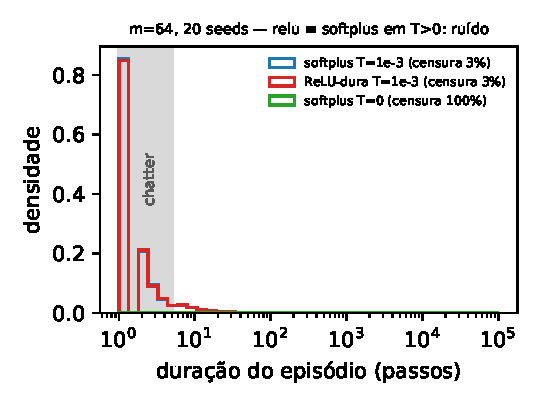
\includegraphics[width=0.72\linewidth]{fig3-diagnostico}
\caption{Why \texttt{etapa-4a} is an instrument negative (post-hoc diagnostic,
$m=64$, 20 seeds). Episode durations as the fraction of episodes per logarithmic
bin; the bands are $\pm1$ standard error across the 20 seeds. At $T=10^{-3}$
hard ReLU (dashed) lies on top of softplus (solid) --- same median of $4$ steps
inside the shaded chatter band, same tail --- which cannot be the zero-gradient
theorem at work, since a dead ReLU unit has exactly zero gradient; these are
noise threshold-crossings. The $T=0$ arm completed only $2$ of its $461$
episodes within the same horizon, so those two are drawn as individual markers
rather than as a density, and the remaining $99.6\%$ are censored at $H=10^{5}$;
that is where the real physics sits and why the confirmatory moved to $T=0$ with
a longer horizon. Script
\protect\path{etapa4-mlp-populacao/figuras_diagnostico.py}.}
\label{fig:diagnostico}
\end{figure}

A redesign, \texttt{etapa-4a.2}, was itself rejected at the design stage by the same
process (commit \texttt{a413b19}): at $T=10^{-5}$ the ReLU-to-softplus ratio
stayed $\approx0.95$ after debounce, because gradient starvation at $\beta=300$
masked the effect, and the pooled null broke $\alpha$ by $30$--$92\times$ in
heterogeneous and autocorrelated worlds. The inheritance was explicit: a
hysteresis and dwell ruler, a per-neuron stratified null, and a move to the
deterministic regime $T=0$ with a much longer horizon. These negatives falsify
neither the area law nor the toy calibration. They falsify two rulers, and they
are what forced the working design.

\subsection{A softplus unit dies and returns in a real MLP, and the area opens
first}\label{sec:mechanism}

Moving to $T=0$ and to a sub-parametrized regime made the mechanism visible. The
regime is the \emph{pressure} pilot: a plateau at $\sim0.15$ on the rich target
$y=\sin(2\pi x)+0.3\sin(5\pi x)$ with $n=16$, $\eta=10^{-3}$ and
$H=2\cdot10^{5}$; 64 runs, commit \texttt{b48b527}, exploratory. Hard ReLU gave a
structural zero: 0 resurrections out of 25 deaths across 16 seeds, so the frozen
branch of \cref{prop:noncomm} is exact in a real network at $T=0$. Softplus
resurrected by mechanism: at $\beta=10$ a unit died at step 781 and returned at
$139\,179$; at $\beta=300$ one died at 3315 and returned at $152\,977$, having
parked shallow enough that the $e^{\beta z}$ channel did not vanish. Both
dynamical resurrections showed the ordered triple
$t_{\mathrm{death}}<t_{\mathrm{area}}<t_{\mathrm{res}}$, so the area law held
$2/2$. The gap between gate and return is the finite-$\beta$ rise time,
$\sim|z_{\mathrm{park}}|/\mathrm{drift}$, rather than the asymptotic $O(1/\beta)$
correction. The bottleneck was quantified as an event rate of $\sim0.1$ per run,
and that number set the entire sizing of the confirmatory.

\Cref{fig:traj3d} shows the $\beta=10$ episode as it happened, in the three
coordinates the theorem talks about: time, margin, accumulated area. The
qualitative shape of \cref{fig:mecanismo} --- dive, sticking layer, debt,
zero of the area, release --- appears in a trained network with no scalar
reduction and no smoothing of the data, only with the return lagging the gate by
the finite-$\beta$ rise time instead of by $O(1/\beta)$. The scope of this
transfer is
narrow: in this episode $68\%$ of the lifetime elapses
\emph{after} the gate opens, so at $\beta=10$ the asymptotic release formula is
far from its regime. What transfers to the trained network is the
\emph{ordering} $t_{\mathrm{death}}<t_{\mathrm{area}}<t_{\mathrm{res}}$ and
the gate's necessity, not the $O(1/\beta)$ release-time expansion.

\begin{figure}[!tbp]
\centering
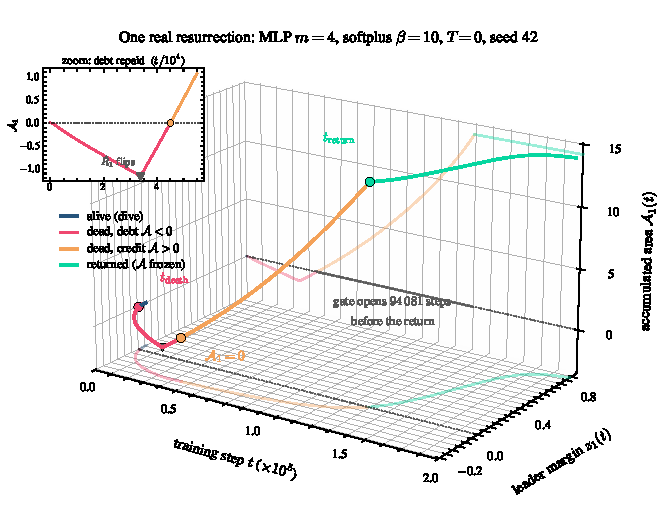
\includegraphics[width=0.88\linewidth]{fig5-trajectory3d}
\caption{One real resurrection, drawn from the recorded trajectory of the run
described above (pressure pilot, softplus $\beta=10$, $m=4$, $n=16$,
$\eta=10^{-3}$, $T=0$, $H=2\cdot10^{5}$, seed 42, unit $k=1$). The axes are the
training step $t$, the leader margin $z_1(t)$ whose sign decides life or death,
and the ruler's accumulated area
$\Ar_1(t)=\eta\sum_{s=\thit}^{t}\hat R_1(s)$; the pale curves on the two walls
are the $(t,z_1)$ and $(t,\Ar_1)$ projections. The unit dives and dies at
$t=781$ ($\thit$). The area then runs into debt while the projected residual
$\hat R_1$ is adverse, turns at $t=33\,905$ where $\hat R_1$ changes sign
(inset), and comes back to zero at $t=45\,098$: the gate. The margin only then
crawls up out of the sticking layer and crosses zero at $t=139\,179$, so the
gate opens $94\,081$ steps before the return --- the ordering
$\thit<t_{\mathrm{area}}<t_{\mathrm{res}}$ of \cref{thm:main}, with the lag
being the finite-$\beta$ rise time. The ruler stops accumulating at the return,
which is why $\Ar_1$ is flat afterwards. Nothing is fitted or smoothed: the
curve is the trajectory itself, sub-sampled every $40$ steps, and the four
marked steps are exact. Script \protect\path{figura_trajetoria3d.py}, which re-runs
the cell and refuses to plot unless the committed triple
$(781,\,45\,098,\,139\,179)$ is reproduced exactly.}
\label{fig:traj3d}
\end{figure}

\subsection{The area law reproduces under a pre-registered
confirmatory}\label{sec:confirmatory}

The confirmatory, \texttt{etapa-4a.3}, was pre-registered at commit \texttt{a8f8f8c} after
two further adversarial rounds, with every design number derived
programmatically from a 240-run rate pilot (commit \texttt{995a87c}); the run is
commit \texttt{5a961cb}. Design grid: $\{$sp-$\beta3$ (primary), sp-$\beta10$,
sp-$\beta300$, ReLU$\}\times m\in\{4,6\}\times50$ held-out seeds
($1900$--$1949$, not used in any pilot), for 400 runs at $T=0$ and
$H=5\cdot10^{5}$. The eligibility window is $[0,307\,536]$, that is $H-\tau$
with $\tau$ the $q_{0.9}$ return time of the pilot. The instrument is a single
ground-truth clock with bit-exact parity to the pilot motor (\cref{alg:regua}),
read by the pre-registered decision procedure of
\cref{alg:decisao,alg:decisao2}, and the area
of the leader-datum residual is accumulated on that clock, so temporal ordering is
structural and the only empirical failure mode of the area test is a return
without area.

\begin{table}[t]
\centering
\caption{Confirmatory 4a.3: 400 runs, 100 per arm, $T=0$, $H=5\cdot10^{5}$.
$\lambda$ is the number of dynamical deaths per run.
$\hat p_{\mathrm{death}}$ conditions on all dynamical deaths in the arm;
$\hat p_{\mathrm{elig}}$ conditions on the deaths that occur inside the
eligibility window $[0,307\,536]$, which is the only conditioning for which the
return is observable within the horizon (for sp-$\beta3$ the eligible denominator
is $N_{\mathrm{elig}}=30$ with 15 returns). Brackets are $95\%$ Clopper--Pearson
intervals, except the $\lambda$ column, which carries a $95\%$ bootstrap interval
clustered by seed. ReLU is the validity control: any ground-truth return there
would invalidate the run.}
\label{tab:4a3}
\small
\begin{tabular}{@{}lccccc@{}}
\toprule
arm & dyn.\ deaths & $\lambda$/run [boot] & returns & $\hat
p_{\mathrm{death}}$ & $\hat p_{\mathrm{elig}}$ \\
\midrule
sp-$\beta3$   & 35 & $0.350\,[0.220,0.500]$ & 16 & $0.457\,[0.288,0.634]$ &
$0.500\,[0.313,0.687]$ \\
sp-$\beta10$  & 27 & $0.270\,[0.160,0.390]$ & 10 & $0.370\,[0.194,0.576]$ &
$0.385\,[0.202,0.594]$ \\
sp-$\beta300$ & 19 & $0.190\,[0.100,0.290]$ & 4  & $0.211\,[0.061,0.456]$ &
$0.222\,[0.064,0.476]$ \\
ReLU          & 17 & $0.170\,[0.090,0.260]$ & 0  & $0.000\,[0.000,0.195]$ &
$0.000\,[0.000,0.195]$ \\
\bottomrule
\end{tabular}
\end{table}

\begin{table}[t]
\centering
\caption{The pre-registered questions of 4a.3, with the condition that kills each
one. All thresholds were derived programmatically from the rate pilot and frozen
in \protect\path{config_4a3.json} at commit \texttt{a8f8f8c}, before the run.}
\label{tab:preregistered}
\small
\begin{tabular}{@{}llll@{}}
\toprule
label & estimand & condition that kills & verdict \\
\midrule
C1 & $p(\mathrm{ret}\mid\mathrm{eligible})$, sp-$\beta3$
   & CP upper $<0.076$, $N_{\mathrm{elig}}\ge10$ & reproduces \\
C2 & returns with area first, sp-$\beta3$
   & CP lower $<0.5$, $\ge6$ returns & sustains \\
C3 & rise gap against park depth
   & none (estimation) & not aggregated \\
C4 & $p(\mathrm{ret}\mid\mathrm{death})$ against $\beta$
   & none (estimation) & monotone in $\beta$ \\
V  & returns in the ReLU arm
   & any single return & clean, $0/17$ \\
\bottomrule
\end{tabular}
\end{table}

The verdicts (\cref{tab:4a3,tab:preregistered,fig:escada}) are as follows.

\begin{itemize}
\item \textbf{C1, existence with rate, primary arm sp-$\beta3$: reproduces.}
With $N_{\mathrm{elig}}=30$ against the floor $n^\ast=10$, there are 15 eligible
returns and $\hat p_{\mathrm{elig}}=0.500\,[0.313,0.687]$, well above the kill
threshold $0.076$. Over all 35 dynamical deaths the same 16 returns give
$\hat p_{\mathrm{death}}=0.457\,[0.288,0.634]$; the two numbers are two
conditionings of one count, not two estimates of one quantity.

\item \textbf{C2, the area law, sp-$\beta3$: sustains.} The leader-drive area
opens before the return in $13/16$ dynamical resurrections, with lower
Clopper--Pearson bound $0.544>0.5$ on $\ge6$ returns. The ordering itself is
partly structural: the clock accumulates the area only on dead steps and closes
at the return, so $t_{\mathrm{area}}<t_{\mathrm{res}}$ cannot fail whenever the
area opens at all (\cref{app:alg1}). The empirical content is that the area in
fact turned positive in $13/16$ cases; the 3 returns without area are real and
are counted against the law: they are returns driven off the
leader datum, which the single-datum hypothesis (H3) does not cover; a
per-datum area $\mathcal A_i$ is the natural extension. What this instrument can
say about the gate stops there, as the post-hoc aggregation of
\cref{app:c3} makes explicit.

\item \textbf{C3, the rise gap: estimation, not aggregated.} C3 was
pre-registered as an estimation-only quantity with no kill condition, relating
the gap $t_{\mathrm{res}}-t_{\mathrm{area}}$ to the park depth
$z_{\mathrm{park}}$ and to the channel $\sigma(\beta z_{\mathrm{park}})$. Those
quantities are recorded per episode by the instrument, but the frozen analysis
script contains no aggregate for C3. A post-hoc aggregation, produced after the
confirmatory data were seen and labelled as such, is reported in
\cref{app:c3}: it finds no evidence that the opening of the area predicts the
return time beyond the onset of the episode. The episode's mean drive was never
persisted by the instrument, which is why the question cannot be pushed
further; persisting the drive series is inherited as a requirement for future
experiments.

\item \textbf{C4, channel staircase: estimation, monotone in $\beta$.}
$\hat p_{\mathrm{death}}$ falls $0.457>0.370>0.211>0.000$ from $\beta=3$ to hard
ReLU, with the intervals of \cref{tab:4a3}. The pairwise intervals overlap;
the pre-registered protocol declared C4 an estimation with no kill condition,
so no trend test was frozen in advance. Conditioning on death when $\beta$ also
moves the death rate ($35/27/19/17$ dynamical deaths across the four arms)
introduces a collider bias in $\hat p_{\mathrm{death}}$; C4 was already
estimation-only, and this note makes the caveat explicit. As \emph{post-hoc
supporting analysis}
we report the Cochran--Armitage trend test across the four ordered arms:
$z=-3.49$, $p=4.9\cdot10^{-4}$ (pairwise Fisher, $\beta=3$ vs.\ ReLU:
$p=8.1\cdot10^{-4}$; $\beta=3$ vs.\ $\beta=300$ alone: $p=0.086$, not
significant --- the trend test, not pairwise comparison, is the appropriate
instrument for an ordered dose--response). Likewise for C2, a post-hoc exact
binomial test of $13/16$ against $0.5$ gives one-sided $p=0.011$ (two-sided
$0.021$); the pre-registered criterion was the Clopper--Pearson bound, which
these tests corroborate but did not replace. The activation smoothness controls
the return channel, and $\beta=3$, the stiffness scale of the GELU family, is the
arm with the highest return probability. This is the direct bridge to the
plasticity practice of \cref{sec:noncomm}.

\item \textbf{Validity: clean.} ReLU gave $0/17$ dynamical returns, which is
\cref{prop:noncomm} measured with $N=100$ runs.
\end{itemize}

\begin{figure}[t]
\centering
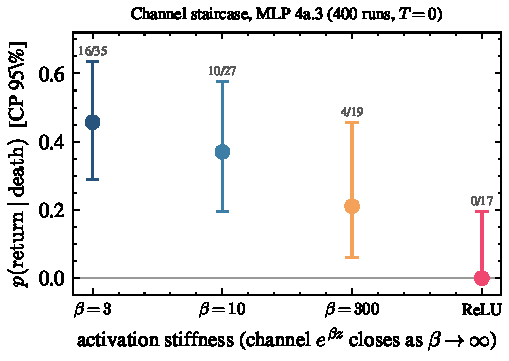
\includegraphics[width=0.72\linewidth]{fig-escada-4a3}
\caption{The channel staircase (C4, confirmatory 4a.3, 400 runs, $T=0$).
$\hat p_{\mathrm{death}}$ is monotone in the activation stiffness and reaches a
structural zero at hard ReLU, where the gradient vanishes identically; the smooth
channel $e^{\beta z}$ closes as $\beta\to\infty$. The fractions above each point
are returns over deaths and the error bars are $95\%$ Clopper--Pearson
intervals. Script \protect\path{figuras_paper.py}.}
\label{fig:escada}
\end{figure}

The limits of the confirmatory are $T=0$, one small architecture, a
one-dimensional rich target, and $m\in\{4,6\}$. The stochastic regime is a paper
of its own (\cref{sec:falsification}). The kill condition of C1 is intentionally
near-unreachable at this $N$, a consequence of the frozen rule that halves the
pilot lower bound, so in practice C2 is the deciding test; this was signalled in
the pre-registration rather than discovered afterwards.

\subsection{The theorem class transfers to a transformer feed-forward
block}\label{sec:transformer}

The same question in a one-layer transformer, for the feed-forward block over an
attended token, does not reduce to the MLP. The scoping run (exploratory, commit
\texttt{d4e4c35}) exposed two mechanisms that reshaped the design, a GELU
sign-flip barrier and an upstream resurrection channel; both are stated in
\cref{sec:transformer-gelu}. The confirmatory therefore tests the theorem class,
softplus-$\beta$, on the block, and treats the barrier and the upstream channel
as estimands of their own.

A rate pilot of 160 runs (commit \texttt{2dba27d}) then fixed the design. Natural
FFN death is $\approx0$, since units with $d=16$ input do not die on their own,
so the confirmatory is necessarily injection-conditional; the non-stationary
channel chatters, forcing the hysteresis instrument of \cref{alg:hist}, with
$\delta_h\approx0.0476$ calibrated from data; and the return time is
slow, $\tau\approx60\,000$--$66\,000$ steps, forcing
$H=2\cdot10^{5}$. The upstream channel was already clean in the pilot: the
difference between training and frozen attention was $+6/+6/+6/+8$ returns, and
ReLU went from $0$ to $8$ with own-move $0$.

\paragraph{The pre-registered protocol.}
A confirmatory run for the transformer was pre-registered at commit
\texttt{1b45498}: 800 runs over
$\{$sp-$\beta3$, sp-$\beta10$, GELU, ReLU$\}\times\{$attn-train,
attn-frozen$\}\times$ injection $\{-0.3,-2.0\}\times50$ seeds $2000$--$2049$,
with $H=2\cdot10^{5}$ and $T=0$. The grid completed with $800/800$ runs
(manifest \path{manifest-e5.json}), with no change to the estimands. The
decision procedure is \cref{alg:decisao,alg:decisao2}. The five pre-registered
estimands E-A
to E-E are stated verbatim in \cref{app:estimands}, so that the protocol is on
record ahead of the data.

\paragraph{The verdicts.}
\Cref{tab:e5} carries the frozen analysis, one row per estimand: the validity
control is clean, the theorem class transfers through the unit's own channel,
the upstream channel reproduces in all four arms, the $\beta$ ordering of the
MLP staircase repeats inside the block, and the GELU barrier is left
consistent-with but confounded with depth. \Cref{app:estimands} keeps each
estimand as it was frozen, with its result attached; \cref{fig:grade-e5} shows
the whole grid at a glance.

\begin{figure}[t]
\centering
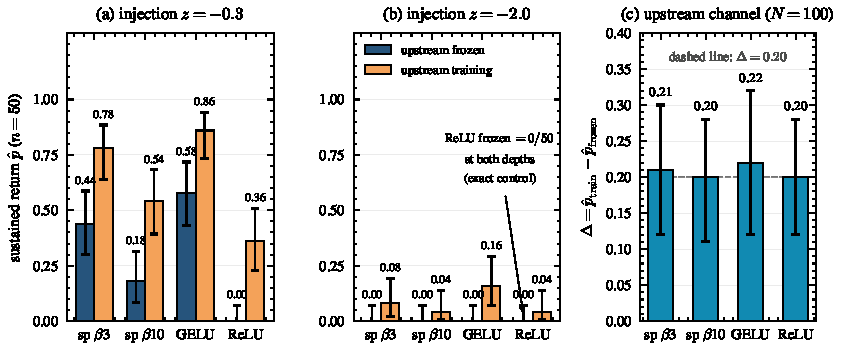
\includegraphics[width=\linewidth]{fig6-grade-e5.pdf}
\caption{The confirmatory grid on the transformer feed-forward block ($800$
runs; $50$ per activation-by-depth-by-regime cell; hysteresis
$\delta_h=0.0476$, horizon $H=2\cdot10^{5}$). (a),\,(b) Sustained-return rate
$\hat p$ with $95\%$ Clopper--Pearson intervals at shallow ($z=-0.3$) and deep
($z=-2.0$) injection. (c) The upstream channel:
$\Delta=\hat p_{\mathrm{train}}-\hat p_{\mathrm{frozen}}$ pooled over both
depths ($100$ runs per arm, $95\%$ bootstrap-by-seed intervals). Three
readings: $\Delta$ is uniform at ${\approx}\,0.20$ across all four
activations, so the upstream channel is not an artefact of any one
nonlinearity; relu-frozen is exactly $0/50$ at both depths, the designed
negative control; and shallow GELU is the highest cell ($0.580$ frozen,
$0.860$ training), consistent with GELU having no dead stratum
(\cref{fig:barreira}). Script \protect\path{figura_grade_e5.py}.}
\label{fig:grade-e5}
\end{figure}

\begin{table}[!t]
\centering
\caption{Transformer confirmatory (\texttt{etapa-5}): 800 runs, $T=0$,
$H=2\cdot10^{5}$, pre-registered at commit \texttt{1b45498}. One row per frozen
estimand; the wording of each target is the pre-registration's, reproduced
verbatim in \cref{app:estimands}. Brackets are $95\%$ Clopper--Pearson
intervals for proportions and $95\%$ bootstrap intervals for the differences
$\Delta$. Denominators are $50$ runs per arm-by-depth cell and $100$ per arm
when the two depths are pooled.}
\label{tab:e5}
\footnotesize
\newcolumntype{L}[1]{>{\raggedright\arraybackslash}p{#1\linewidth}}
\begin{tabular}{@{}L{0.11}L{0.20}L{0.29}L{0.30}@{}}
\toprule
estimand & pre-registered target & result & interval or test \\
\midrule
E-A, validity
 & no sustained return in the relu-frozen arm
 & valid: $0/100$ sustained returns, both depths
 & --- (a single return would have invalidated the run) \\
\addlinespace
E-B, upstream channel
 & $\Delta=p_{\mathrm{sust}}(\mathrm{train})-p_{\mathrm{sust}}(\mathrm{frozen})$
   with positive bootstrap lower bound, per arm
 & reproduced in all four arms: $0.210$ (sp-$\beta3$), $0.200$
   (sp-$\beta10$), $0.220$ (GELU), $0.200$ (ReLU)
 & $[0.120,0.300]$; $[0.110,0.280]$; $[0.120,0.320]$; $[0.120,0.280]$. ReLU
   contrast $20/100$ against $0/100$, two-sided Fisher exact test,
   $p=6.6\cdot10^{-7}$ \\
\addlinespace
E-C, transfer of the theorem class
 & at least $n^\ast=6$ sustained returns, sp-$\beta3$ frozen, shallow injection
 & transferred: $22/50$ sustained returns, $3.7\times$ the gate; the leader-drive
   area opened before the return in $21/22$
 & $\hat p=0.440\,[0.300,0.587]$; gate $n^\ast=6$ \\
\addlinespace
E-D, GELU barrier
 & shallow injection far above deep in the own channel, against a depth-matched
   control
 & consistent with the barrier, confounded with depth (the frozen three-way
   label): GELU $29/50$ shallow against $0/50$ deep, but sp-$\beta3$ deep also
   gives $0/50$
 & S1 signature, $\mathrm{sign}(\Ar_{\mathrm{drive}})\neq
   \mathrm{sign}(\Ar_{\mathrm{mlp}})$, in $92\%$ of deep against $4\%$ of
   shallow episodes \\
\addlinespace
E-E, $\beta$ staircase
 & estimation across $\beta\in\{3,10\}$, frozen and training, no kill condition
 & $\beta=3$ above $\beta=10$ in both factors: frozen $0.220$ against $0.090$,
   training $0.430$ against $0.290$; GELU is the most revivable arm
 & GELU shallow frozen $0.580\,[0.432,0.718]$; with the upstream channel
   $0.860\,[0.733,0.942]$ \\
\bottomrule
\end{tabular}
\end{table}

\subsection{GELU sits outside the class and the moving input opens a second
channel}\label{sec:transformer-gelu}

The scoping run of the block (commit \texttt{d4e4c35}) produced two facts that
are mechanisms in their own right, and that the confirmatory above carries as
E-D and E-B:

\begin{itemize}
\item \textbf{S1, a GELU sign-flip barrier.} $\mathrm{GELU}'(z)$ changes sign at
$z^\ast=-0.7518$, verified analytically: for $z<z^\ast$ it is negative, so a
deep-dead unit is pushed away from the return by its own gradient.
Self-resurrection is possible only in the shallow band $(-0.752,0)$;
\cref{fig:barreira} draws the barrier and both injection depths. The MLP's
blind area port, which omits $g'$, gets the sign wrong on $12/12$ GELU episodes;
the correct instrument uses the slope-weighted area $\Ar_{\mathrm{drive}}$. GELU
is therefore genuinely outside the monotone-sigmoid class of \cref{thm:main}.
There is a prior point: GELU has no dead stratum to begin with. A unit at margin
$-0.3$ emits $\mathrm{GELU}(-0.3)=-0.115\ne0$ and keeps contributing to the
residual, so $\{z\le0$ on every datum$\}$ is not a singular stratum for GELU but
a region of weak, sign-inverted coupling. The sign-flip barrier is the symptom
that the definition of death does not apply, and it is consistent with GELU
being the most revivable arm we measured (shallow frozen $0.580$); we note that
against sp-$\beta3$-frozen ($29/50$ against $22/50$) the difference is not
statistically separable, two-sided Fisher exact test, $p=0.23$.

\begin{figure}[t]
\centering
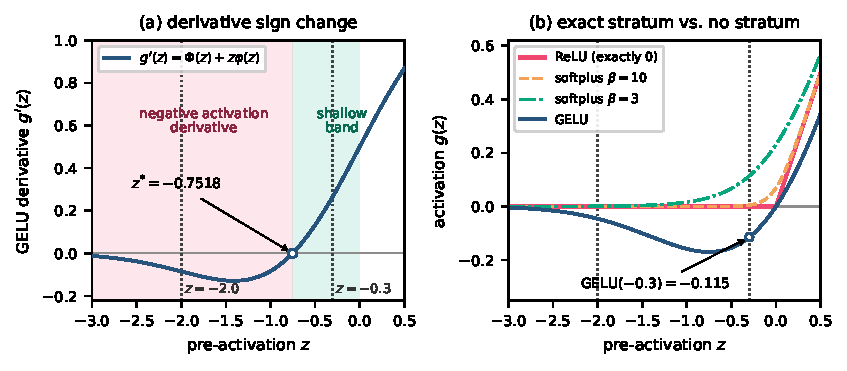
\includegraphics[width=\linewidth]{fig7-barreira-gelu.pdf}
\caption{The analytic barrier and the non-stratum, both exact. Left: the GELU
derivative $g'(z)=\Phi(z)+z\varphi(z)$ changes sign at $z^\ast=-0.7518$; below
$z^\ast$ (shaded) the unit's own gradient is adverse and the region is
self-trapping, while on the shallow band $(z^\ast,0)$ the own gradient still
points back toward activity. The two injection depths of the confirmatory,
$z=-0.3$ and $z=-2.0$, sit on opposite sides of the barrier. Right: the
activations themselves. ReLU vanishes identically for $z<0$, an exact dead
stratum; softplus-$\beta$ is exponentially small but strictly positive; GELU
is strictly negative, with $\mathrm{GELU}(-0.3)=-0.115$, so for GELU there is
no dead stratum at all and the deep-injection suppression of
\cref{fig:grade-e5} must come from the sign of $g'$, not from a loss of rank.
Script \protect\path{figura_barreira_gelu.py}.}
\label{fig:barreira}
\end{figure}

\item \textbf{S2, an upstream channel.} The input of the block,
$h=e+\mathrm{attn}(e)$, is non-stationary, so a hard-ReLU unit whose own gradient
is identically zero can still revive because $h$ moves. With attention frozen the
control is exact: the margin change is $0.000$ and the own-move is $0$. With
attention training the own-move is still $0$, yet the margin climbs by $+0.69$ on
average and by up to $+1.32$. The MLP statement ``dead ReLU is terminal'' holds
only when the input is fixed; the transformer adds a channel the MLP does not
have.
\end{itemize}

Neither mechanism is a technicality of the instrument. The barrier says that the
MLP mechanism does not port unchanged to a GELU block, since the sign-flip
obstructs self-resurrection below $z^\ast$; the upstream channel says that
terminality of a discretely dead unit is a statement about that unit's own
channel under a stationary input, and nothing more. In the confirmatory the
barrier's terminality could not be separated from injection depth, and it is
reported that way (E-D of \cref{tab:e5}); the upstream channel is established in
all four arms (E-B).

\paragraph{The deep zero is what the channel law predicts.} The own channel of
sp-$\beta3$ is $\sigma(3z)$, which is $0.289$ at the shallow injection
$z=-0.3$ and $0.00247$ at the deep one $z=-2.0$: a ratio of about $117$. The
return time measured in the shallow cells is $\tau\approx60\,000$--$66\,000$
steps, so scaling it by that ratio projects a deep return at roughly
$7\cdot10^{6}$ steps, about $35$ times the horizon $H=2\cdot10^{5}$. The
$0/50$ of sp-$\beta3$ frozen at $z=-2.0$ is therefore predicted by the channel
law itself, at this horizon, and is not a failure of the transfer. It also
disarms part of the E-D confound: the deep suppression of softplus is
starvation of a quantitatively predicted size, so the depth-matched control
gives $0/50$ for a reason that has nothing to do with the GELU barrier, and
the two mechanisms remain separable only by the depth sweep around
$z^\ast=-0.752$ that \cref{app:estimands} specifies.

\subsection{Deviations from the pre-registered protocol}\label{sec:deviations}

(i) None for 4a.3: the analysis frozen at \texttt{a8f8f8c} was run unchanged at
\texttt{5a961cb}, and the validity control passed.
(ii) The eligibility window $[0,307\,536]$, the kill threshold $0.076$, the
floor $n^\ast=10$ for C1 and the floor of $\ge6$ returns for C2 were all derived
programmatically from the rate pilot (\texttt{995a87c}) and frozen in
\path{config_4a3.json} before the run; none was chosen after seeing the
confirmatory data.
(iii) C3 was pre-registered as estimation-only; the frozen script reports no
aggregate for it, and the post-hoc aggregation of \cref{app:c3} is labelled as
such (\cref{sec:confirmatory}).
(iv) For the transformer, the pre-registered package was revised once before
freezing: an earlier candidate was rejected in adversarial review for a
confound between injection depth and the GELU barrier, and was replaced by the
package of commit \texttt{1b45498}, which adds a depth-matched control. No run
was executed under the rejected package.

\section{Limitations}\label{sec:limits}

\textbf{(i)} The theorem is proved for the minimal configuration: one unit, one
active datum at a time, a fixed readout and a one-dimensional input. Every
constant is verified on a reference instance and the release law holds on
$57/57$ of the admissible instances of a 600-draw sweep (\cref{sec:sweep}), with
a residual bias, $55/57$ measured offsets smaller in modulus than predicted,
that we read as the $o(\beta^{-1})$ remainder at finite $\beta$. \Cref{thm:forcing}
removes the restriction to one live unit --- the live side may be any affine
subsystem of order $m$ --- but not the others: the readout is still fixed, and
the experiments train $v_k$. The resulting gradation is (P1)--(P3) of
\cref{sec:intro}, and \cref{cor:mlp} is the level at which the transfer is
deduced rather than measured; the transfer to the experiments as run remains
empirical, and we are explicit about this rather than treating the two as the
same object.
\textbf{(i$'$)} One step of the proof is open, and it is inherited rather than
created by the forcing form: the $o(1)$ in the entry-corner estimate of
\cref{lem:corner-in} is not quantified, so the remainder of \eqref{eq:release}
is $o(\beta^{-1})$ and not the $O(\log\beta/\beta^2)$ the numerics suggest. It
has a concrete empirical signature in the measured regression slope, and the
competing explanation was excluded numerically; the argument and the numbers are
(O3) of \cref{app:forcing-open}.
\textbf{(i$''$)} Two further constraints of \cref{thm:forcing} are scope and not
debt, and are declared as such: the constancy of the live activation pattern
(\cref{rem:H4F}), whose relaxation costs an exponential in $m$ ((O2) of
\cref{app:forcing-open}), and the threshold $\beta_0$, exhibited as a chain of
five explicit conditions (\cref{tab:beta0}) with the binding ones linear in $m$
and deliberately not composed into a single number. What is genuinely
uncontrolled there is not the $m$-dependence but the \emph{forcing} dependence,
as (O1) of \cref{app:forcing-open} states.
\textbf{(i$'''$)} The trainable readout is the one restriction that separates
the proved object from the experiments as run; it is (O6) of
\cref{app:forcing-open}.
\textbf{(ii)} The regime is $T=0$ deterministic gradient flow throughout the
theorem and the confirmatory; the stochastic gate is open and, where probed,
falsifies the deterministic schedule (\cref{sec:falsification}), since late
captures recur past the deterministic window at a rate the reduced stochastic
model under-predicts, leaving the reactivating unit's back-reaction as the
leading candidate driver.
\textbf{(iii)} Scale: the confirmatories are small networks ($m\le6$ MLP units,
$m_{\mathrm{ffn}}=4$ block units) with rich one-dimensional targets, chosen so
that a single unit can be tracked with a ground-truth clock.
\textbf{(iv)} GELU is outside the monotone class; its own-channel revival is
blocked below $z^\ast=-0.752$, and in the confirmatory the barrier could not be
separated from depth (the pre-registered three-way label), because at the deep
injection $z=-2.0$ the softplus own channel is starved to $0.9\%$ of its shallow
value --- a factor of about $117$, which projects the deep return past $35$
horizons (\cref{sec:transformer-gelu}) --- while $\mathrm{GELU}'$ is adverse, so
both mechanisms predict the same zero at this horizon; the separating design,
a sweep of injection depths around
$z^\ast=-0.752$, is stated in \cref{app:estimands} and left as future work. The
upstream channel is established; the barrier's terminality remains open.
\textbf{(v)} The cone apex, of corank $\ge2$, where weight decay produces genuine
sliding toward the most singular stratum, is untouched.
\textbf{(vi)} The independence of the law from the smoothing is proved for
softplus and verified numerically for erf; it is not proved for the whole
monotone-sigmoid class.

\section{Conclusion}\label{sec:conclusion}

We derived an entry--exit law for the death and resurrection of a smoothed unit,
verified each of its constants on a two-neuron instance, and tested the release
law over a sweep of 600 drawn instances, where it holds on all 57 that satisfy
the hypotheses, with a median relative error of $2.7\%$. The law belongs to the
forcing: \cref{thm:forcing} extends it to any live subsystem of the affine
class with $m$ units, with constants uniform to $O(\sqrt m)$ and
$\beta_0=O(m)$ (\cref{prop:beta0}), verified over $66+23+67$ further
instances; this converts the bridge to an MLP of the class from analogy into
a corollary under a-posteriori-verifiable hypotheses (\cref{cor:mlp}), with
the trainable readout remaining the empirical level (P3). We measured the law
in a small MLP under a pre-registered protocol: resurrection occurs, the residual
area opens before the return in 13 of 16 cases, hard ReLU gives a structural
zero, and the return probability is monotone in the activation stiffness. In a
pre-registered transformer confirmatory the theorem class transferred to
the feed-forward block through the own channel ($22/50$, area before the return
in $21/22$), a second upstream channel reproduced in all four arms, and GELU's
sign-changing derivative left its signature in $92\%$ of deep episodes while its
terminality remained confounded with depth --- the pre-registered three-way
label, reported as frozen.

What this is, and is not. The value of the law is understanding: it replaces
``dead units are terminal'' with a mechanism --- a gate with memory --- in the
regime where the mechanism is provable. It is not a training tool. The
asymptotics live on the channel $e^{\beta z}$ being exponentially small, and one
would expect an adaptive optimizer that divides by the running RMS of the
gradient to rescale precisely that smallness. An exploratory pilot on the toy
instances (13 instances, \path{e7-adam-portao} in the repository) measured
this expectation instead of assuming it, and it fails in an instructive way:
under Adam the gate survives, parked deeper by the optimizer's floor --- the
release moves to where the channel crosses $\epsilon$, empirically
$\beta z_{\mathrm{park}}\approx-\ln(1/\epsilon)+\mathrm{const}$ --- and the
area law itself reappears as $\epsilon$ grows, with relative error $0.24\%$ at
$\epsilon=1$ against $0.017\%$ for plain gradient descent. This is a pilot,
not a confirmatory, and momentum-rich production regimes remain unmeasured. What does
transfer is smaller and sharper: the sign structure of the activation
derivative, which is an exact fact about GELU (\cref{sec:transformer-gelu})
and, with the zero at $z^\ast=-1.2785$ instead of $-0.7518$, about SiLU; the
calibrated-null instrument of \cref{sec:negatives}, which any measurement of
rare events in training can reuse; and the folklore correction that the
terminality of discrete death is a statement about stationary input. The
cheapest consequential experiment this paper points at is not a scaling of the
theorem but a histogram: the mass of feed-forward pre-activations below
$z^\ast$ in production-scale models, and whether that mass is sticky across
training.

\section{Reproducibility}\label{sec:repro}

All code, configs, per-run manifests and aggregate JSON needed to reproduce
every number and figure in this note are in a single Git repository. One
policy governs the raw data, in both confirmatories: the per-episode trace
files (\path{results-4a3/*.jsonl.gz}, \path{results-e5/*.jsonl.gz}) are kept
out of version control, while the manifests that checksum them
(\path{results-4a3/manifest-4a3.json}, \path{results-e5/manifest-e5.json}) are
versioned. The traces are byte-reproducible from the pinned configs
(deterministic single-threaded CPU runs), so the versioned SHA256 list is what
makes a regenerated file verifiable. That repository is private at the time of
writing, so the commit hashes below, while they resolve in it and fix the
state of every experiment, are not independently checkable today; public
release under the MIT licence is a precondition for submission. All runs are
deterministic on CPU with per-run manifests (SHA256, git hash, config), and
pre-registration commits precede every confirmatory run in the repository
history. No external data were used; every dataset in this note is generated
by the scripts listed below.

{\sloppy
\begin{itemize}
\item \textbf{Theorem constants and figures.} \path{06-notas/t2-prova/}: lemma
verifications \texttt{passo0--6.py} and \texttt{prova\_L1--L6.py}; figures via
\path{figuras_draft.py}. The forcing theorem is drafted standalone in
\path{06-notas/t2-prova/teorema-forcing-draft.tex}, which is the mathematical
source of \cref{sec:forcing,app:forcing}; its two adversarial referee reports
are \path{05-experimentos/t2-n-neuronios/parecer-14.md} and
\path{05-experimentos/t2-n-neuronios/parecer-15.md}.
\item \textbf{Forcing theorem, numerics (\cref{sec:forcing-numerics}).}
\path{05-experimentos/t2-n-neuronios/}: the $m$-sweep, the cloning replica and
the unit-readout family are \path{verifica_forcing.py} (outputs
\path{forcing_m.jsonl}, \path{controle_dt.jsonl}, log \path{run_forcing.log});
the regressions and the unit-readout family are \path{parecer14.py}, the $\beta$
sweep is \path{beta.py}, and the two pre-hit exponents of \cref{tab:o5} are
\path{parecer15_o5.py} and \path{parecer15_o5b.py}. Those last three campaigns
originally reported to standard output only; their outputs are serialized by the
wrapper \path{gera_artefatos.py}, which invokes them unchanged and writes
\path{unit_readout_m.jsonl} (unit-readout family, one record per evaluated
instance, with the screening counts), \path{beta_sweep.jsonl} (the six worst
$m=8$ instances at $\beta=10^4$ and $3\cdot10^4$) and \path{o5_prehit.jsonl}
(the twelve instances of \cref{tab:o5}, all four $\beta$ each).
\item \textbf{MLP mechanism (pilot).}
\path{etapa4-mlp-populacao/pilotos-4a2/pressao/} (the \emph{pressure} regime:
sub-parametrized, plateau $\sim0.15$); commit \texttt{b48b527}. The trajectory of
\cref{fig:traj3d} is re-run and plotted by
\path{06-notas/paper/figura_trajetoria3d.py}, which asserts the committed
triple before drawing anything; the diagnostic of \cref{fig:diagnostico} is
\path{etapa4-mlp-populacao/figuras_diagnostico.py}.
\item \textbf{MLP confirmatory (4a.3).} \path{.../pressao/taxa/} (the
event-rate pilot and the confirmatory built on it): pre-registration
\texttt{a8f8f8c}, run \texttt{5a961cb}.
\texttt{python run\_4a3.py --workers 4} then \texttt{python analise\_4a3.py},
which reads \path{results-4a3/} and \path{config_4a3.json}. Rate pilot
\texttt{995a87c}. Staircase figure: \path{06-notas/paper/figuras_paper.py}.
\item \textbf{Transformer (\texttt{etapa-5}).} Directory
\path{05-experimentos/etapa5-transformer/}; scoping \texttt{d4e4c35}, rate
pilot \texttt{2dba27d}, confirmatory
pre-registration \texttt{1b45498}.
\texttt{python run\_e5.py --workers 4} then \texttt{python analise\_e5.py}.
\item \textbf{Negatives.} \path{05-experimentos/NEGATIVOS.md} (the register of
negative results) and the \texttt{etapa-4a} note record the invalidated instrument
(commit \texttt{6411ac8}) and the rejected redesign (\texttt{a413b19}); the
falsified schedule is \path{p5-relu-morte-v2/} (commit \texttt{190d94a}).
\end{itemize}
\par}

\paragraph{Compute.}
Every run is single-threaded CPU on an Intel Core i9-9900K, with 4 concurrent
workers through Python \texttt{multiprocessing} at \texttt{nice 19} and no GPU;
the only dependency is \texttt{numpy} (Python 3.14, numpy 2.4). The 4a.3
confirmatory, 400 runs at $H=5\cdot10^{5}$, took $4.9$ h wall-clock, that is
$19.5$ CPU-hours at $175$ s per run. The transformer confirmatory, 800 runs at
$H=2\cdot10^{5}$, took $13.9$ h wall-clock, which includes one stall of the
runner and its resumption. The verification of the forcing theorem
(\cref{sec:forcing-numerics}) is cheap by comparison: the $m$-sweep, the
cloning replica, the unit-readout family, the $\beta$ sweep on the six worst
instances and the twelve RK4 pre-hit integrations add about $1$ h wall-clock in
total on the same machine, single-threaded. The preliminary and discarded
runs, namely \texttt{etapa-4a} (600 runs), the \texttt{4a.2} redesign, the
pressure pilot (64
runs) and the two rate pilots (240 and 160 runs), are of the same order again and
are not otherwise reported.

\section*{Acknowledgments}
This work received no funding and was carried out independently. The author
declares no competing interests.

\section*{Data availability}
Everything needed to reproduce every number and figure --- code, configs,
per-run manifests and aggregate JSON --- is held at the commits cited in
\cref{sec:repro}, under the trace-file policy stated there. The repository is
not public at the time of writing; no external data were used.

\section*{Declaration of LLM usage} Large language models were used throughout
the work: to draft and copy-edit the text, to run the adversarial reviews, to
write the experiment and verification code, and to work out the derivations of
\cref{app:lemmas}. The hypotheses, the pre-registered kill conditions, the
decision to declare a design or a hypothesis dead, and the reading of the
cited sources are the author's.

A review that only re-read the derivation would be circular, so the checks
that carry weight here are the ones that do not read it. Each lemma is
re-derived symbolically from scratch by a committed script (SymPy), which
recomputes the identity rather than confirming the prose; the convergence
table \cref{tab:dt} refines the integrator until the measured coefficient
meets the proved one; and the sweep of \cref{sec:sweep} confronts the release
law with 600 independently drawn trajectories. These routes test the law
against the dynamics, not against the text that describes it, and any of them
can fail while the prose stands. The central identity, \cref{lem:gauge}, is in
addition a computation of about ten lines and is presented in that form so
that a reader can redo it by hand.

\begin{thebibliography}{99}

\bibitem{Sokar23} G.~Sokar, R.~Agarwal, P.~S.~Castro, U.~Evci, \emph{The dormant
neuron phenomenon in deep reinforcement learning}, in: Proceedings of the 40th
International Conference on Machine Learning, PMLR 202 (2023) 32145--32168.
arXiv:2302.12902.

\bibitem{Lyle23} C.~Lyle, Z.~Zheng, E.~Nikishin, B.~Avila Pires, R.~Pascanu,
W.~Dabney, \emph{Understanding plasticity in neural networks}, in: Proceedings of
the 40th International Conference on Machine Learning, PMLR 202 (2023)
23190--23211. arXiv:2303.01486.

\bibitem{Dohare24} S.~Dohare, J.~F.~Hernandez-Garcia, Q.~Lan, P.~Rahman,
A.~R.~Mahmood, R.~S.~Sutton, \emph{Loss of plasticity in deep continual
learning}, Nature 632 (2024) 768--774. doi:10.1038/s41586-024-07711-7.

\bibitem{HG16} D.~Hendrycks, K.~Gimpel, \emph{Gaussian error linear units
(GELUs)}, preprint (2016), arXiv:1606.08415.

\bibitem{DMS16} P.~De Maesschalck, S.~Schecter, \emph{The entry--exit function
and geometric singular perturbation theory}, J.~Differential Equations 260 (2016)
no.~8, 6697--6715. doi:10.1016/j.jde.2016.01.008.

\bibitem{EJRW23} S.~Eberle, A.~Jentzen, A.~Riekert, G.~S.~Weiss, \emph{Existence,
uniqueness, and convergence rates for gradient flows in the training of
artificial neural networks with ReLU activation}, Electron.\ Res.\ Arch.\ 31
(2023) no.~5, 2519--2554. doi:10.3934/era.2023128. arXiv:2108.08106.

\bibitem{Fil88} A.~F.~Filippov, \emph{Differential Equations with Discontinuous
Righthand Sides}, F.~M.~Arscott (ed.), Mathematics and Its Applications, Kluwer,
Dordrecht, 1988. doi:10.1007/978-94-015-7793-9.

\bibitem{SDR23} M.~Sensi, M.~Desroches, S.~Rodrigues, \emph{Slow--fast dynamics
in a neurotransmitter release model: delayed response to a time-dependent input
signal}, Physica D 455 (2023) 133887. doi:10.1016/j.physd.2023.133887.
arXiv:2302.12852.

\bibitem{Jef16} M.~R.~Jeffrey, \emph{Exit from sliding in piecewise-smooth flows:
deterministic vs.\ determinacy-breaking}, Chaos 26 (2016) no.~3, 033108.
doi:10.1063/1.4943386.

\bibitem{GH15} N.~Guglielmi, E.~Hairer, \emph{Classification of hidden dynamics
in discontinuous dynamical systems}, SIAM J.~Appl.\ Dyn.\ Syst.\ 14 (2015)
no.~3, 1454--1477. doi:10.1137/15100326X.

\bibitem{GH22} N.~Guglielmi, E.~Hairer, \emph{An efficient algorithm for solving
piecewise-smooth dynamical systems}, Numer.\ Algorithms 89 (2022) no.~3,
1311--1334. doi:10.1007/s11075-021-01154-1.

\bibitem{ST98} J.~Sotomayor, M.~A.~Teixeira, \emph{Regularization of
discontinuous vector fields}, in: L.~Magalh\~aes, C.~Rocha, L.~Sanchez (eds.),
Equadiff 95: Proceedings of the International Conference on Differential
Equations (Lisboa 1995), World Scientific, Singapore, 1998, pp.~207--223.

\bibitem{LST07} J.~Llibre, P.~R.~da Silva, M.~A.~Teixeira, \emph{Regularization
of discontinuous vector fields on $\mathbb{R}^3$ via singular perturbation},
J.~Dynam.\ Differential Equations 19 (2007) no.~2, 309--331.
doi:10.1007/s10884-006-9057-7.

\bibitem{Kri17} K.~U.~Kristiansen, \emph{Blowup for flat slow manifolds},
Nonlinearity 30 (2017) no.~5, 2138--2184. doi:10.1088/1361-6544/aa6449.
arXiv:1603.01821.

\bibitem{KS01} M.~Krupa, P.~Szmolyan, \emph{Extending geometric singular
perturbation theory to nonhyperbolic points---fold and canard points in two
dimensions}, SIAM J.~Math.\ Anal.\ 33 (2001) no.~2, 286--314.
doi:10.1137/S0036141099360919.

\bibitem{BP21} J.~Bolte, E.~Pauwels, \emph{Conservative set valued fields,
automatic differentiation, stochastic gradient method and deep learning},
Math.\ Program.\ 188 (2021) no.~1, 19--51. doi:10.1007/s10107-020-01501-5.
arXiv:1909.10300.

\bibitem{Lu20} L.~Lu, Y.~Shin, Y.~Su, G.~E.~Karniadakis, \emph{Dying ReLU and
initialization: theory and numerical examples}, Commun.\ Comput.\ Phys.\ 28
(2020) no.~5, 1671--1706. doi:10.4208/cicp.OA-2020-0165. arXiv:1903.06733.

\bibitem{CP34} C.~J.~Clopper, E.~S.~Pearson, \emph{The use of confidence or
fiducial limits illustrated in the case of the binomial}, Biometrika 26 (1934)
no.~4, 404--413. doi:10.1093/biomet/26.4.404.

\bibitem{WT11} M.~Welling, Y.~W.~Teh, \emph{Bayesian learning via stochastic
gradient Langevin dynamics}, in: Proceedings of the 28th International Conference
on Machine Learning (ICML 2011), 2011, pp.~681--688.

\end{thebibliography}

\appendix
\section{Proofs of the six lemmas}\label{app:lemmas}

Each proof closes with the outcome of its committed executable verification. The
scripts are symbolic where an identity is claimed and numerical where a rate or a
constant is claimed; they are listed in \cref{sec:repro}. Throughout,
$\sigma(s)=1/(1+e^{-s})$, $w=e^{\beta z}$, $u=1/w$ and $\Psi(u)=\log u+u$, and we
use freely the elementary identities $\sigma(\beta z)=1/(1+u)$,
$\beta\,g_\beta(z)=\log(1+w)$ and $(1-\sigma(s))/\sigma(s)=e^{-s}$, all of which
are verified symbolically in \path{passo0_verificacao.py}.

\subsection{Normal form and additive quadrature}\label{app:L1}

\begin{lemmarep}{lem:gauge}{normal form and additive quadrature}
Let $w=e^{\beta z}$ and $u=1/w$, and set $\Psi(u)=\log u+u$. In fast time
$\tau=\beta t$ the margin obeys
\begin{equation*}
\frac{dw}{d\tau}=c\,R(t)\,\frac{w^{2}}{1+w}\,(1+E_\beta),
\qquad
|E_\beta|\le\frac{\log(1+w)}{\beta|R|},
\tag{\ref{eq:normalform}}
\end{equation*}
the quadratic normal form of De Maesschalck and
Schecter~\cite[equations~(1.9)--(1.10)]{DMS16} with $\varepsilon=\beta^{-1}$,
and one has the exact additive
identity
\begin{equation*}
\frac{d\Psi(u)}{dt}=-c\,\beta\,R(t)+c\log(1+w)+\mathcal{E}_{\eqref{H3}}(t),
\qquad
\bigl|\mathcal{E}_{\eqref{H3}}\bigr|\le C_3\,\beta\,e^{-\beta\delta_1}.
\tag{\ref{eq:quadrature}}
\end{equation*}
Under \eqref{H1}--\eqref{H2} the additive correction satisfies
$\int_{\thit}^{\trel}c\log(1+w)\,ds=O(\log\beta/\beta)$.
\end{lemmarep}

\begin{proof}[Proof of \cref{lem:gauge}]
\emph{Step 1 (margin equation, exact under \eqref{H3}).}
$\dot z=(x_j,1)\cdot\dot\theta_A$, and the field on $\theta_A$ is
$-\tfrac1n\sum_i\mathrm{res}_i\,\sigma(\beta z_i)(x_i,1)$. The term $i=j$
contributes $-c\,(g_\beta(z)-R)\,\sigma(\beta z)$, because
$\mathrm{res}_j=g_\beta(z)-R$ by the definition \eqref{eq:residual} of $R$; the
terms $i\ne j$ are bounded by $C_3'e^{-\beta\delta_1}$ by the scalar reduction of
\cref{lem:corner-out}. Hence
$\dot z=-c(g_\beta(z)-R)\sigma(\beta z)+O(e^{-\beta\delta_1})$, which in the
gauge $w$ and fast time $\tau=\beta t$ is \eqref{eq:normalform}.

\emph{Step 2 (exact chain rule).} $\dot u=-\beta u\,\dot z$ and
$\Psi'(u)=(1+u)/u$; together with $\sigma(\beta z)=1/(1+u)$,
\[
\frac{d\Psi}{dt}
=\frac{1+u}{u}\cdot(-\beta u)\cdot
\Bigl[-c\bigl(g_\beta(z)-R\bigr)\tfrac{1}{1+u}\Bigr]
=c\,\beta\,\bigl(g_\beta(z)-R\bigr).
\]

\emph{Step 3 (additive identity).} Since $\beta\,g_\beta(z)=\log(1+e^{\beta z})
=\log(1+w)$, substitution gives $d\Psi/dt=-c\beta R+c\log(1+w)$, plus the
\eqref{H3} error of Step~1 carried through the same factors, which is bounded by
$C_3\beta e^{-\beta\delta_1}$. This is \eqref{eq:quadrature}. No division by $R$
occurs, so the interior zero of $R$ forced by \eqref{H1}--\eqref{H2} through the
intermediate value theorem is harmless.

\emph{Step 4 (bound on the correction, in three windows).} On the episode
$w=1/u$ with $u=c\beta|\Ar(t)|(1+o(1))$ away from neighbourhoods of the endpoints
(\cref{lem:release}(i)). In the bulk, where $|\Ar|\ge a_0(\delta)$, one has
$\log(1+w)\le w\le 1/(c\beta a_0)$, so that stretch contributes at most
$\Tep/(\beta a_0)=O(\beta^{-1})$, where $\Tep=\texit-\thit$ is the duration of the
episode, not the training horizon $H$: the bulk stretch lies inside the episode by
construction. Near $\thit$ and $\texit$ the function $\Ar$ has
transversal zeros, with derivatives $cR(\thit)\ne0$ and $cR(\texit)\ne0$, so
$|\Ar(t)|\ge\kappa|t-t_\ast|$ locally and
\[
\int\log(1+w)\;\lesssim\;\int_{1/\beta}^{\epsilon}\frac{ds}{c\beta\kappa s}
=\frac{\log(\beta\epsilon)}{c\beta\kappa};
\]
on the $O(\beta^{-1})$-wide stretches glued to the endpoints one has $w=O(1)$ and
$\log(1+w)\le\log2+O(1)$, contributing $O(\beta^{-1})$. Summing the three windows
gives $O(\log\beta/\beta)$ with constant
$C_4=2/\bigl(c\min(|R(\thit)|,R(\texit))\bigr)+\Tep/a_0$.
\end{proof}

\begin{remark}[consequence used downstream]\label{rem:L1cons}
Integrating \eqref{eq:quadrature} gives
$\Psi(u(t))=\Psi(u_0)-c\beta\Ar(t)+O(\log\beta/\beta)$ uniformly on the episode.
This is the form that sustains the depth $u=c\beta|\Ar|(1+o(1))$ on compacts and
the release at $\texit+O(\beta^{-1})$, and it is what
\cref{lem:release,lem:bootstrap} consume.
\end{remark}

\noindent\emph{Verification.} \path{prova_L1_verificacao.py} confirms the
additive identity symbolically, and the integral correction with the normalized
metric is stable in $[8.2,10.6]$, below the leading theoretical term
$2/\bigl(cR^{\hyb}(\texit)\bigr)=2/(0.625\times0.108)=29.6$, for
$\beta\in[3\cdot10^2,10^4]$. The full theoretical constant adds the bulk term:
with $\Tep=\texit-\thit=1.1325-0.1114=1.021$ and $a_0\approx0.02$ in the instance,
$C_4=29.6+1.021/0.02=80.7$. Using the training horizon $H=1.7$ in place of $\Tep$
would give $114.6$ instead; the bound of \cref{lem:gauge} is over the episode,
so $\Tep$ is the correct length.

\subsection{The \texorpdfstring{$B$}{B}-subsystem and the feedback}\label{app:L2}

\begin{lemmarep}{lem:gronwall}{$B$-subsystem and feedback}
Under \eqref{H4} the $B$-field is affine with Lipschitz constant
$L_B=\lambda_{\max}(G_B)$, where $G_B$ is the Gram matrix of the active data, and
$R^{\hyb}$ is affine in $\theta_B$. Integral Gr\"onwall consuming the bound of
\cref{lem:gauge} gives, conditionally on the layer being maintained (supplied by
\cref{lem:bootstrap}),
\begin{equation*}
\sup\bigl\|\theta_B^\beta-\theta_B^{\hyb}\bigr\|=O\!\left(\frac{\log\beta}{\beta^{2}}\right),
\tag{\ref{eq:Brate}}
\end{equation*}
one full order better than the naive $O(\beta^{-1})$: in the bulk
$u=O(\beta|\Ar|)$, so the coupling is $O(\beta^{-2})$ there and $O(\beta^{-1})$
only in the $O(\beta^{-1})$-wide corner windows.
\end{lemmarep}

\begin{proof}[Proof of \cref{lem:gronwall}]
\emph{Step 1 (\eqref{H4} makes the field linear).} With the activation pattern
constant, the $B$-field is $-G_B(\theta_B-\theta_B^\ast)$ with $G_B$ the Gram
matrix of the active data, hence $C^\infty$ with Lipschitz constant
$L_B=\lambda_{\max}(G_B)$, equal to $2.13$ in the reference instance. Moreover
$R^{\hyb}=y_j-(x_j,1)\cdot\theta_B$ is affine in $\theta_B$ and $C^1$ in $t$,
with $\|\dot R^{\hyb}\|_\infty\le\|(x_j,1)\|\,\|G_B\|\,\mathrm{diam}=:C_R$
explicit.

\emph{Step 2 (coupling bound).} The perturbation caused by $A$ in
$\mathrm{res}_i$ is $g_\beta(z_{A,i})$. Under \eqref{H3} the terms $i\ne j$
contribute $C_3e^{-\beta\delta_1}$ and the term $i=j$ contributes $g_\beta(z)$;
the Gram factors give a constant $C_f$, so
$\|G_A(t)\|\le C_f\,g_\beta(z(t))+C_3e^{-\beta\delta_1}$.

\emph{Step 3 (integral Gr\"onwall).} Writing $\Delta=\theta_B^\beta-\theta_B^{\hyb}$
we have $\dot\Delta\le L_B\Delta+\|G_A\|$, hence
$\Delta(t)\le\int e^{L_B(t-s)}\|G_A(s)\|\,ds$, and therefore
\[
\sup_{[t_{\mathrm{cross}},\trel]}\|\Delta\|
\;\le\;e^{L_BH}\Bigl[\tfrac{C_f}{c\beta}\int c\log(1+w)\,dt
+H\,C_3e^{-\beta\delta_1}\Bigr].
\]
Since $g_\beta=\beta^{-1}\log(1+w)$ and \cref{lem:gauge} gives
$\int c\log(1+w)\,dt=O(\log\beta/\beta)$, the total is $O(\log\beta/\beta^{2})$,
which is \eqref{eq:Brate}. Consequently $R^\beta=R^{\hyb}+O(\log\beta/\beta^{2})$,
which is the perturbation size consumed by \cref{lem:bootstrap}.
\end{proof}

\noindent\emph{Verification.} \path{prova_L2_verificacao.py} confirms that the
field and $R$ are affine with $L_B=2.133$, that the margins of \eqref{H4} hold
with $\min z_B=0.39$, and that the refined rate holds: the metric
$\sup\cdot\beta^{2}/\log\beta$ is stable in $[4.2,5.7]$ over
$\beta\in[3\cdot10^2,3\cdot10^3]$. The exponent is what the metric discriminates:
under a pure $O(\beta^{-1})$ the same metric would grow like $\beta/\log\beta$,
by a factor of about $6.5$ per decade, and it grew by a factor of $1.24$.

%mesmos beta em que a linha de Status do mesmo arquivo (e o draft-v3) reportam
%o intervalo [4.20,5.70]. Adotei [4.2,5.7] por ser o numero que ja circula no

\subsection{The entry corner}\label{app:L3}

\begin{lemmarep}{lem:corner-in}{entry corner}
Let $v=c\,|R^{\hyb}(\thit)|$ be the arrival speed, transversal by \eqref{H1}. The
exact identity $(1-\sigma(s))/\sigma(s)=e^{-s}$ collapses the crossing-time
difference to an elementary integral and gives
\begin{equation*}
t_{\mathrm{cross}}^{\beta}=\thit+\frac{1}{\beta v}\bigl(1+O(\delta_z)+o(1)\bigr),
\qquad
\bigl\|\theta^\beta(t_{\mathrm{cross}})-\theta^\infty(\thit)\bigr\|=O(\beta^{-1}),
\tag{\ref{eq:corner-in}}
\end{equation*}
where $t^\beta_{\mathrm{cross}}$ is the first time with $w=w_0$. The
exponentially weighted approach integral is $\tfrac{3/2}{\beta v}(1+o(1))$, the
factor $3/2$ coming from $\int_0^\infty e^{-s}(1+e^{-s})\,ds$.
\end{lemmarep}

\begin{proof}[Proof of \cref{lem:corner-in}]
\emph{Step 1 (pre-corner with exponential weight).} For $z\ge\delta_z$ one has
$|g_\beta(z)-z|\le\beta^{-1}e^{-\beta z}$ and $1-\sigma(\beta z)\le e^{-\beta z}$,
so the inhomogeneity of the Gr\"onwall comparison against the ReLU flow is
$h(t)\le Ce^{-\beta z^0(t)}$. Near the hit, transversality gives
$z^0(t)=v\,(\thit-t)(1+O(\delta_z))$, hence
\[
\int h\,dt\;\le\;C\!\int e^{-\beta v(\thit-t)}\,dt\;\le\;\frac{C}{\beta v}.
\]
Along the real trajectory the weight carries in addition the factor $\sigma$ from
the layer, and the exact value is
$\int e^{-\beta z}dt=\tfrac{1}{\beta v}\int_0^\infty e^{-s}(1+e^{-s})\,ds\,(1+o(1))
=\tfrac{3/2}{\beta v}(1+o(1))$.

The weight is self-consistent by a monotone route, with no exponential fixed
point. Since $e^{-\beta z}$ is decreasing in $z$, the flow whose inhomogeneity is
evaluated at any sub-solution $z_-\le z^\beta$ majorizes the true inhomogeneity.
Iterate: $z^{(0)}=z^{0}$, and let $z^{(k+1)}$ solve the problem with weight
$e^{-\beta z^{(k)}}$. The iteration is monotone decreasing and bounded below by
the ReLU sub-solution with slack $2C/(\beta v)$: the increment of each step is at
most $C/(\beta v)\cdot\sup e^{\beta(z^{(k)}-z^{(k+1)})}$, and while
$|z^{(k)}-z^{(k+1)}|\le1/\beta$ that factor is at most $e$, a bound maintained by
the size of the increment itself, by induction on $k$. The iteration therefore
converges to $z^\beta$ with $\Delta\theta(t_\delta)=O(1/(\beta v))$, without
requiring a fixed-point inequality of the form $C_2e^{c'K}\le K$.

\emph{Step 2 (window-crossing identity).} On $[0,\delta_z]$ the crossing speeds
are $v_0(z)=v(1+O(\delta_z))$ for ReLU and
$v_\beta(z)=v_0(z)\sigma(\beta z)+O(\beta^{-1})$ for softplus, so the difference
of crossing times is
\begin{align*}
\int_0^{\delta_z}\!\Bigl(\frac{1}{v_\beta}-\frac{1}{v_0}\Bigr)dz
&=\frac{1}{v}\int_0^{\delta_z}\frac{1-\sigma(\beta z)}{\sigma(\beta
z)}\,dz\,(1+O(\delta_z))\\
&=\frac{1}{v}\int_0^{\delta_z}e^{-\beta z}\,dz\,(1+O(\delta_z))
=\frac{1-e^{-\beta\delta_z}}{\beta v}(1+O(\delta_z)),
\end{align*}
where the middle equality is the exact identity
$(1-\sigma(s))/\sigma(s)=e^{-s}$. With $w_0=1$ there is no further shift, since
$\log w_0=0$. Adding Steps~1 and~2 gives
$t_{\mathrm{cross}}-\thit=\tfrac{1}{\beta v}(1+O(\delta_z)+o(1))$, and the speeds
are bounded on the window, so the state at crossing is within $O(\beta^{-1})$ of
$\theta^\infty(\thit)$.
\end{proof}

\noindent\emph{Verification.} \path{prova_L3_verificacao.py} confirms the two
identities symbolically and both constants numerically:
$K_{\mathrm{teo}}=1/v=7.042$ against $K_{\mathrm{emp}}=7.127$ refitted from the
measured crossing times, a deviation of $1.2\%$; and the exponentially weighted
approach integral with the exact factor $3/2$ gives $10.563$ in theory against
$10.52$ measured, below $1\%$.

\subsection{Sticking and release for prescribed forcing}\label{app:L4}

\begin{lemmarep}{lem:release}{sticking and release for prescribed $R$}
Let $R\in C^1$ be prescribed and satisfy \eqref{H1}--\eqref{H2}, and write
$\Ar(t)=\int_{\thit}^{t}R$. Then

(i) $\Psi(u(t))=\Psi(u_0)-c\beta\Ar(t)+\mathrm{corr}(t)$ with
$0\le\mathrm{corr}(t)=\int c\log(1+w)\,ds=O(\log\beta/\beta)$; on compact
subintervals of $(\thit,\texit)$,
$u=c\beta|\Ar(t)|\bigl(1+O(\log\beta/(\beta a_0))\bigr)$, so the sticking depth is
$z\sim-\beta^{-1}\log\beta$;

(ii) the release obeys the closed formula
\begin{equation*}
\trel-\texit=\frac{\mathrm{corr}(\beta)}{c\,\beta\,R(\texit)}\,(1+o(1))
=O\!\left(\frac{\log\beta}{\beta^{2}}\right),
\tag{\ref{eq:release-prescribed}}
\end{equation*}
so $u$ returns to $O(1)$ at $\texit+O(\beta^{-1})$, with no $\log\beta$ factor;

(iii) a perturbation $\tilde R=R+\delta$ shifts $\texit$ by at most
$\delta\,(\texit-\thit)/R(\texit)+O(\delta^{2})$.

No division by $R$ occurs anywhere: the layer is held by the area, not by the
sign of $R$, and the interior zero of $R$ forced by \eqref{H1}--\eqref{H2} is
harmless.
\end{lemmarep}

\begin{proof}[Proof of \cref{lem:release}]
\emph{Step 1 (monotone comparison).} The right-hand side of
$\dot\Psi=-c\beta R+c\log(1+w(\Psi))$ is decreasing in $\Psi$, because $w=1/u$
and $u$ is increasing in $\Psi$. The Chaplygin comparison principle therefore
applies: $R_1\le R_2$ implies $\Psi_1\ge\Psi_2$, and piecewise-constant envelopes
of $R$ give sub- and super-solutions that are exactly integrable through the same
primitive $\Psi$, hence with explicit constants.

\emph{Step 2 (depth, item (i)).} Integrate the exact identity
\eqref{eq:quadrature}; the correction is bounded by \cref{lem:gauge}, in the same
three windows. On compact subintervals of $(\thit,\texit)$ one has $u$ large, so
$\Psi(u)=u(1+o(1))$ and the depth law $u=c\beta|\Ar(t)|(1+o(1))$ follows, that is
$z\sim-\beta^{-1}\log\beta$.

\emph{Step 3 (release, item (ii)).} At release $\Psi$ returns to its entry value
$\Psi(u_0)$, so the constant $\Psi(u_0)$ cancels and no spurious term survives;
item~(i) then gives $c\beta\Ar(\trel)=\mathrm{corr}(\trel)$. By \eqref{H2} the
zero of $\Ar$ at $\texit$ is transversal, with
$\Ar(t)=R(\texit)(t-\texit)(1+o(1))$, and solving for $\trel$ gives
\eqref{eq:release-prescribed}. The delay of the release is exactly the correction
integral of \cref{lem:gauge}, reparametrized by the exit speed.

\emph{Step 4 (perturbation, item (iii)).} Apply the implicit function theorem to
$\Ar_{\tilde R}(t)=0$ with denominator $R(\texit)\ne0$, splitting the episode into
the same three windows: near the hit $|\Ar|\ge|R(\thit)|s/2$ for $s=t-\thit$
small, in the bulk $|\Ar|\ge a_0(\delta)$, and near the exit the zero is
transversal. This gives the shift
$\le\delta\,(\texit-\thit)/R(\texit)+O(\delta^{2})$.
\end{proof}

\begin{remark}[the corollary that explains the coupled constant]\label{rem:L4cor}
In the coupled system the initial datum comes from the entry corner, so by
\cref{lem:corner-in} the episode starts with a delay $K/\beta$ that cuts an
initial negative area $\approx R(\thit)K/\beta$. Item (ii) then gives
$\beta\,(\trel-\texit^{\hyb})\to-K\,|R(\thit)|/R(\texit)$. With the theoretical
$K=1/(c|R(\thit)|)$ this is exactly $-1/(cR(\texit))=-14.81$, the
coefficient of \eqref{eq:release} left by the cancellation; with the
empirical $K=7.13$ it is
$-(7.13\times0.2272)/0.1080=-15.0$, against $-14.38$ measured, a deviation of
$4\%$ whose residue is the positive correction of item~(ii).
\end{remark}

\noindent\emph{Verification.} \path{prova_L4_verificacao.py} measures $\trel$
and $\mathrm{corr}$ on the same run and tests
$\Delta t=\mathrm{corr}/(c\beta R_{\mathrm{exit}})$: the formula closes to
$0.2\%/1.0\%/9.5\%$ at $\beta=3\cdot10^2/10^3/3\cdot10^3$ on a grid of
$2\cdot10^{-6}$, the last figure having collapsed from $35\%$ to $9.5\%$ under a
fivefold grid refinement, which identifies the residue as discretization. The
corollary of \cref{rem:L4cor} closes at $-14.99$ against $-14.38$ measured
($4.2\%$).

\subsection{The coupled bootstrap}\label{app:L5}

\begin{lemmarep}{lem:bootstrap}{coupled bootstrap}
Under \eqref{H1}--\eqref{H4} the coupled system satisfies the two-term law
\begin{equation*}
t^\beta_{\mathrm{release}}
=\texit-\frac{1}{c\,R^{\hyb}(\texit)}\cdot\frac{1}{\beta}
+\frac{\mathrm{corr}(\beta)}{c\,\beta\,R^{\hyb}(\texit)}+o(\beta^{-1}),
\qquad \mathrm{corr}(\beta)=O\!\left(\frac{\log\beta}{\beta}\right),
\tag{\ref{eq:twoterm}}
\end{equation*}
obtained by continuation with strict margins, with the constant
$M_2=e^{L_BH}C_fC_4/c$ independent of the continuation hypothesis for
$\beta\ge\beta_0$. In the first-order coefficient the arrival speed cancels: in
the product $K\,|R^{\hyb}(\thit)|/R^{\hyb}(\texit)$ of the entry delay by the
area it cuts, the factor $|R^{\hyb}(\thit)|$ cancels against
$K=1/(c|R^{\hyb}(\thit)|)$ of \cref{lem:corner-in}, leaving a coefficient that
still depends on $c$ and on $R^{\hyb}(\texit)$.
\end{lemmarep}

\begin{proof}[Proof of \cref{lem:bootstrap}]
The argument is a continuation with strict margins.

\emph{Step 1 (the bootstrap property).} For $s$ in
$[t_{\mathrm{cross}},\texit-\varepsilon_\beta]$ let $\mathcal P_s$ be the
property that, on $[t_{\mathrm{cross}},s]$, (a)
$\sup\|\theta_B^\beta-\theta_B^{\hyb}\|<2M_2\log\beta/\beta^{2}$ and (b)
$z(t)<\beta^{-1}\log w_0-\beta^{-1}$ for $t\ge
t_{\mathrm{cross}}+C_{\mathrm{collar}}/\beta$.
The collar is necessary: at $t_{\mathrm{cross}}$ the margin crosses
$\beta^{-1}\log w_0$ continuously, so the layer can only be strict after an
$O(\beta^{-1})$ entry window. The constant is
$M_2=e^{L_BH}C_fC_4/c$, explicit through the chain \cref{lem:gronwall} composed
with \cref{lem:gauge}.

\emph{Step 2 (nonempty and open).} \Cref{lem:corner-in} supplies the initial
datum with slack: the state is within $O(\beta^{-1})$ in $\theta$ and the layer is
reached transversally, so $\mathcal P_s$ holds for $s$ just past the collar. All
quantities in $\mathcal P_s$ are continuous in $s$, since the trajectories are
$C^1$, so the strict inequalities propagate to a neighbourhood.

\emph{Step 3 (improvement, hence closed).} Assume $\mathcal P_s$ with the
constant $2M_2$. Since $R$ is affine in $\theta_B$ (\cref{lem:gronwall}(a)), the
forcing satisfies $R^\beta=R^{\hyb}+\delta$ with
$\|\delta\|\le\mathrm{Lip}_R\cdot2M_2\log\beta/\beta^{2}$. The sandwich of
\cref{lem:release} with perturbed forcing then keeps
$u(t)\ge c\beta(|\Ar(t)|-\|\delta\|H)/2>u_0$ for $t\le\texit-\varepsilon_\beta$
with $\varepsilon_\beta=C_\varepsilon\log\beta/\beta$ and
$C_\varepsilon=4C_4/(cR_{\mathrm{exit}})$, so the layer is maintained with a
margin. With the layer in hand, the Gr\"onwall of \cref{lem:gronwall} is
unconditional and returns $M_2$, half of what was assumed, for an explicit
$\beta\ge\beta_0$. The threshold $\beta_0$ is finite and traceable through the
chain of constants, though we do not exhibit it. Crucially $M_2$ does not depend
on the hypothesis $2M_2$, because the chain of constants is unconditional; this
is what closes the bootstrap.

\emph{Step 4 (continuation).} The set of $s$ for which $\mathcal P_s$ holds is
nonempty (Step~2), open (strict margins and continuity) and closed (the bounds
pass to limits) in $[t_{\mathrm{cross}},\texit-\varepsilon_\beta]$, hence it is
the whole interval.

\emph{Step 5 (terminal window).} On
$[\texit-\varepsilon_\beta,\trel]$ apply \cref{lem:release}(ii)--(iii) with the
forcing frozen at $R^{\hyb}+O(\log\beta/\beta^{2})$. Three contributions add: the
displacement caused by $\delta$ is $O(\log\beta/\beta^{2})$ by item (iii); the
correction delay is $+\mathrm{corr}/(c\beta R_{\mathrm{exit}})$ by item (ii); and
the area cut at entry, $\int_{\thit}^{\thit+K/\beta}R\approx R(\thit)K/\beta$,
advances the exit by $-K|R(\thit)|/(R(\texit)\beta)=-1/(cR(\texit)\beta)$, the
arrival speed cancelling against $K=1/(c|R(\thit)|)$. Summing gives
\eqref{eq:twoterm}.
\end{proof}

\noindent\emph{Verification.} \path{prova_L5_verificacao.py} checks that the
two-term law reproduces the whole coupled sweep, with deviations
$1.9\%/0.7\%/0.2\%/0.1\%$ for $\beta=3\cdot10^2\ldots10^4$, and that
the surviving
coefficient is $1/(cR_{\mathrm{exit}})=14.815$; the chain of constants is
exhibited with $M_2=440.8$ from the empirical $C_4=10.6$, against
$M_2\le1233$ from the leading theoretical term $2/(cR^{\hyb}(\texit))=29.6$ alone
and $M_2\lesssim3300$ from the full theoretical $C_4=80.7$, which adds the
bulk term $\Tep/a_0$ with $\Tep=\texit-\thit=1.021$ and $a_0\approx0.02$ in the
instance. The strict layer is
confirmed at $\beta=10^4$. One honest caveat: with the conservative
$C_\varepsilon$ the inner window of the layer check is empty for
$\beta\le3\cdot10^3$, so the check is vacuous there, and at those $\beta$ the
maintenance of the layer is implied only by the detection of the release itself.

\subsection{The exit corner, branch selection and the scalar reduction}\label{app:L6}

\begin{lemmarep}{lem:corner-out}{exit corner, branch selection and scalar reduction}
Under \eqref{H1}--\eqref{H4}, after release: (i) the $\beta$-trajectory crosses
the exit corner in time $\tfrac{1}{\beta v'}(1+o(1))$ with
$v'=c\,R^{\hyb}(\texit)>0$, the mirror of \cref{lem:corner-in}; (ii) the ReLU flow
restarted at $(\theta_A(\thit),\theta_B^{\hyb}(\texit))$ has forward uniqueness on
the activating branch, and that branch is selected by the limit itself, the
frozen Filippov branch~\cite{Fil88} being incompatible with release at
$\texit+O(\beta^{-1})$; (iii) classical Gr\"onwall glues on $[\trel,H]$ at rate
$O(\log\beta/\beta)$. Under \eqref{H3} the other data contribute
$O(e^{-\beta\delta_1})$, the face-$j$ field is rank one along $(x_j,1)$, and the
episode reduces to the scalar problem.
\end{lemmarep}

\begin{proof}[Proof of \cref{lem:corner-out}]
\emph{Step 1 (item (i)).} Mirror \cref{lem:corner-in}, replacing $v$ by
$v'=cR^{\hyb}(\texit)>0$, which is transversal by \eqref{H2}. The crossing
identity is the same, and the weight is $\tfrac{3/2}{\beta v'}$.

\emph{Step 2 (item (ii), forward uniqueness and branch selection).} At the
restart point the active field is locally Lipschitz on the side $z\ge0$ and
$\dot z(\texit^+)=v'>0$, so the solution enters $\{z>\epsilon t\}$ and Picard
uniqueness holds forward from any $t>\texit$. The only Filippov
alternative~\cite{Fil88}, namely remaining in $z\le0$ where the field is
identically zero, is incompatible with the limit of the $\theta^\beta$, since
\cref{lem:bootstrap} places the release at $\texit+O(\beta^{-1})$. The selection
of the activating branch is therefore proved by \cref{lem:bootstrap} and not
postulated in \cref{def:hybrid}.

\emph{Step 3 (item (iii), gluing).} The initial datum of the gluing satisfies
$\|\theta^\beta(\trel)-\theta^\infty(\texit)\|=O(\beta^{-1}\log\beta)$: the
position of $\theta_A$ in the layer contributes $O(\log\beta/\beta)$, $\theta_B$
contributes the rate of \cref{lem:gronwall}, and the time displacement
$O(\beta^{-1})$ contributes through bounded speeds. In the active interior the
two fields are exponentially close, so classical Gr\"onwall on $[\trel,H]$ keeps
the gap at $O(\log\beta/\beta)$.

\emph{Step 4 (scalar reduction).} The field on $\theta_A$ is
$-\tfrac1n\sum_i\mathrm{res}_i\,\sigma(\beta z_i)(x_i,1)$. Under \eqref{H3}, that
is $z_{A,i}\le-\delta_i<0$ for $i\ne j$ on the limit episode, the terms $i\ne j$
are bounded by $Ce^{-\beta\delta_i}$ and are absorbed by the Gr\"onwall estimates
without changing any $O(\beta^{-1})$ rate. The term $i=j$ is rank one along
$(x_j,1)$, so the component of $\theta_A$ tangential to the face is frozen at the
exponential rate, while the normal component is exactly the scalar problem of
\crefrange{lem:gauge}{lem:bootstrap}. Hypothesis \eqref{H3} is an open condition
on the data and the initialization, and it is verified numerically in the
instance with an explicit margin $\delta_1$.
\end{proof}

\noindent\emph{Verification.} \path{prova_L6_verificacao.py} measures the
gluing directly: for $\beta\in\{10^3,3\cdot10^3\}$ the supremum of
$\|\theta^\beta-\theta^{\mathrm{relu}}\|$ over $[\trel+0.05,H]$ is
$1.6\cdot10^{-3}$ and $5.5\cdot10^{-4}$, so the metric $\sup\cdot\beta/\log\beta$
is stable at $0.21$--$0.23$, confirming the rate $O(\log\beta/\beta)$.
\path{passo6_verificacao.py} confirms the scalar reduction: \eqref{H3} holds
with $\delta_1=0.508$ and the tangential drift is below $10^{-10}$, machine zero,
at both values of $\beta$, consistent with $e^{-\beta\delta_1}\sim10^{-65}$.

The debugging of this script is worth recording, because it exhibits the
alternative branch. The first version of the reference restarted the ReLU flow at
$z_A=-1.1\cdot10^{-6}$, an overshoot of one Euler step of the pre-hit loop, and
fell into the frozen Filippov branch, with a constant gap of $\approx0.039$. The
correct reference requires exact projection onto the face together with an
activating nudge larger than the overshoot. Branch selection is a real condition
of the statement.

\section{Proof of the forcing theorem}\label{app:forcing}

This appendix proves \cref{thm:forcing}. It is a rewrite of
\crefrange{lem:gauge}{lem:corner-out} with the residual $R$ treated as a
prescribed forcing generated by an arbitrary live subsystem of the affine class
of \cref{sec:forcing}, instead of by a single live neuron. Each lemma below
carries a \emph{provenance} line saying what is inherited from
\cref{app:lemmas} and what is new. Where the provenance says \emph{identical
with $R$ generic}, we do not reproduce the proof: the audited claim is that the
proof of \cref{app:lemmas} never uses the structure of $B$, only
\eqref{H0p}--\eqref{H2p}, and reproducing it verbatim would add nothing. Where the
provenance says \emph{new}, the proof is written out in full. Only one lemma,
\cref{lem:gronwallF}, changes substantively, and it changes in our favour.

Throughout, $X_{\max}=\max_i\|(x_i,1)\|$, $\|a\|_2=(\sum_{k\ge1}a_k^2)^{1/2}$,
$\Tep=\texit-\thit$, and $\tcross$ is the first time at which $w=w_0$. We use
repeatedly the elementary bounds, valid for all $z$,
\begin{equation}\label{eq:softdefectF}
0\le g_\beta(z)-z_+\le\beta^{-1}e^{-\beta|z|},
\qquad
\bigl|\sigma(\beta z)-\mathbf 1_{\{z>0\}}\bigr|\le e^{-\beta|z|},
\qquad
\beta g_\beta(z)=\log(1+w),
\end{equation}
with $w=e^{\beta z}$, $u=1/w$, $\Psi(u)=\log u+u$, $\sigma(s)=1/(1+e^{-s})$,
$\sigma(\beta z)=1/(1+u)$ and $(1-\sigma(s))/\sigma(s)=e^{-s}$.

\subsection{L1$'$: normal form and additive quadrature}\label{app:F1}

\begin{lemma}[normal form and additive quadrature, forcing form]\label{lem:gaugeF}
With $w=e^{\beta z}$, $u=1/w$, $\Psi(u)=\log u+u$ and $\tau=\beta t$,
\begin{equation}\label{eq:normalformF}
\frac{dw}{d\tau}=c\,R(t)\,\frac{w^2}{1+w}\,(1+E_\beta),
\qquad |E_\beta|\le\frac{\log(1+w)}{\beta|R|},
\end{equation}
and one has the exact additive identity
\begin{equation}\label{eq:quadratureF}
\frac{d\Psi(u)}{dt}=-c\beta R(t)+c\log(1+w)+\mathcal E(t),
\qquad
|\mathcal E(t)|\le C_3\beta e^{-\beta\delta_1}.
\end{equation}
Under \textup{\eqref{H1p}--\eqref{H2p}},
$\int_{\thit}^{\trel}c\log(1+w)\,ds\le C_4\log\beta/\beta$ with $C_4$ as in
\eqref{eq:M2F}.
\end{lemma}

\noindent\emph{Provenance: identical to \cref{lem:gauge} with $R$ generic.}
Step~1 uses only $\res_j=g_\beta(z)-R$, which is the \emph{definition} of $R$,
and the scalar reduction (\cref{lem:corner-outF}, step~4), which is a statement
about the other margins of $A$; steps~2--3 are algebra in $(\Psi,u,\sigma)$;
step~4 bounds the correction in three windows using only $R(\thit)\ne0$,
$R(\texit)\ne0$ and $|\Ar|\ge a_0$ in the bulk, and produces $C_4$ written
purely in terms of $R$. No line mentions $B$. The proof is unchanged; we record
only that $\Tep$, not $H$, is the correct length in the bulk term, since the
bound is taken over the episode.

\subsection{L2$'$: the live subsystem, a PSD energy estimate}\label{app:F2}

\begin{lemma}[live subsystem and feedback, PSD form]\label{lem:gronwallF}
Assume \textup{\eqref{H4p}}, \textup{\eqref{H5p}}, and, on $[\thit,s]$, the layer bound
$\int_{\thit}^{s}c\log(1+w)\,dt\le 2C_4\log\beta/\beta$ supplied by
\cref{lem:bootstrapF}. Put $\Delta=\theta_B^\beta-\theta_B^{\hyb}$. Then
\begin{equation}\label{eq:BrateF}
\sup_{[0,s]}\|\Delta\|
\;\le\;\underbrace{\frac{C_fC_4}{c}\cdot\frac{2\log\beta}{\beta^2}}_{\text{episode}}
\;+\;\underbrace{O(\beta^{-2})}_{\text{pre-hit}}
\;+\;\underbrace{H\Bigl(C_3e^{-\beta\delta_1}
   +C_5\sqrt m\,C_{\mathrm{res}}\,e^{-\beta\delta_B}\Bigr)}_{\text{beyond all orders}} ,
\end{equation}
so $\sup\|\Delta\|=O(\log\beta/\beta^2)$ with constant $M_2=C_fC_4/c$, and
consequently
\begin{equation}\label{eq:RpertF}
R^\beta=R^{\hyb}+\delta,\qquad
\|\delta\|_\infty\le\mathrm{Lip}_R\sup\|\Delta\|
+\frac{m}{\beta}e^{-\beta\delta_B} .
\end{equation}
\emph{No factor $e^{L_BH}$ occurs, and $\lambda_{\max}(G_B)$ does not appear.}
Moreover the same PSD estimate applies after release: on $[\trel,H]$, where both
the $\beta$-flow and $\theta^\infty$ have $A$ alive with the same frozen
pattern, one has \eqref{eq:ivB}, again with no exponential factor (step~5).
\end{lemma}

\noindent\emph{Provenance: new proof.} \Cref{lem:gronwall} obtains the same rate
through the integral Gr\"onwall
$\|\Delta(t)\|\le\int e^{L_B(t-s)}\|G_A(s)\|\,ds$, paying $e^{L_BH}$ with
$L_B=\lambda_{\max}(G_B)$; with unit readouts $\lambda_{\max}(G_B)$ grows like
$m$, so that route makes $M_2$ exponential in $m$ and the theorem vacuous for
large $m$. The observation below is that the sign of $G_B$ is available and
Gr\"onwall throws it away. Step~2b, the live-unit discrepancies, has no
counterpart in \cref{lem:gronwall}.

\begin{proof}
\emph{Step 1 (exact perturbed linear system on the episode).} On $[\thit,H]$ the
hybrid freezes $\theta_A$ at the value with $z=0$, so $A$'s contribution to the
hybrid residuals is \emph{exactly} zero: $\mathrm{ReLU}(z)=0$ on the face $j$ by
construction, and $\mathrm{ReLU}(z_{A,i})=0$ on the other data because their
margins are $\le-\delta_1<0$ by \eqref{H4p} --- a ReLU is not approximately zero
there, it is zero. The $O(e^{-\beta\delta_1})$ that appears below belongs to the
$\beta$-flow, where the softplus of $A$ leaks $\beta^{-1}e^{-\beta\delta_1}$
into each of those residuals; it is a term of $G_A$, not a defect of the hybrid.
The hybrid $B$-flow is therefore exactly
$\dot\theta_B^{\hyb}=-G_B\theta_B^{\hyb}+b$. In the $\beta$-flow the same
computation applies with two extra sources: the output of $A$, which enters
every residual, and the softplus defects of the live units themselves. Hence
\begin{equation}\label{eq:Deltaode}
\dot\Delta=-G_B\Delta+G_A(t)+G_S(t),
\end{equation}
where, with $\varphi_i$ the feature vectors of \eqref{eq:gramF},
\[
G_A(t)=-\frac1n\sum_{i=1}^n g_\beta\bigl(z_{A,i}(t)\bigr)\varphi_i,
\qquad
G_S(t)=\text{(live softplus defect, bounded in step 2b).}
\]
Equation \eqref{eq:Deltaode} is an identity, not an estimate: the affine class
makes the drift exactly linear with the \emph{same} matrix $G_B$ for both flows,
which is why the difference of the drifts is $-G_B\Delta$ with no remainder.

\emph{Step 2a (bound on $G_A$).} Write $C_f=\|\varphi_j\|/n$. By \eqref{H4p} the
margins $z_{A,i}$, $i\ne j$, are $\le-\delta_1$, so those terms contribute at
most $C_3e^{-\beta\delta_1}$; the term $i=j$ is $C_fg_\beta(z)$. Hence
\begin{equation}\label{eq:GA}
\|G_A(t)\|\le C_f\,g_\beta(z(t))+C_3e^{-\beta\delta_1}
=\frac{C_f}{\beta}\log\bigl(1+w(t)\bigr)+C_3e^{-\beta\delta_1}.
\end{equation}
Nothing in \eqref{eq:GA} depends on $m$ except through $C_f$: the size of the
perturbation that $A$ injects is a property of $A$.

\emph{Step 2b (the live-unit discrepancies; new term).} The $\beta$-flow's
$B$-field is, per unit $k$,
\[
-\frac1n\sum_i\res_i\,a_k\,\sigma(\beta z_{k,i})\,(x_i,1),
\]
whereas the hybrid uses $a_k\mathbf 1_{\{z_{k,i}>0\}}(x_i,1)$; and $\res_i$
itself contains $\sum_ka_kg_\beta(z_{k,i})$ where the hybrid has
$\sum_ka_k(z_{k,i})_+$. By \eqref{H4p} every live margin satisfies
$|z_{k,i}|\ge\delta_B$, so \eqref{eq:softdefectF} gives, per unit and per datum,
a derivative defect $\le e^{-\beta\delta_B}$ and an output defect
$\le\beta^{-1}e^{-\beta\delta_B}$. Using \eqref{H5p} to bound $|\res_i|\le
C_{\mathrm{res}}$ and $\|(x_i,1)\|\le X_{\max}$, the $2m$-vector $G_S$ obeys
\begin{equation}\label{eq:GS}
\|G_S(t)\|\;\le\;
\underbrace{\Bigl(\sum_{k=1}^m a_k^2\Bigr)^{1/2}X_{\max}}_{\le\,\|a\|_2X_{\max}}
\Bigl(C_{\mathrm{res}}+\tfrac{m}{\beta}\max_k|a_k|X_{\max}\Bigr)e^{-\beta\delta_B},
\end{equation}
the crude count being $mn$ scalar discrepancies, each $O(e^{-\beta\delta_B})$,
recombined into a Euclidean norm.

We do \emph{not} absorb the second bracket into a $(1+o(1))$. That step would be
hiding a condition on $\beta$ inside asymptotic notation: the bracket collapses
to $C_{\mathrm{res}}(1+o(1))$ only when
\begin{equation}\label{eq:beta2}
\beta\ \ge\ \beta_2:=\frac{m\max_k|a_k|X_{\max}}{C_{\mathrm{res}}},
\end{equation}
that is only for $\beta\gtrsim m$. This is a genuine condition of the theorem
and it is recorded as row~5 of \cref{tab:beta0}; it is, together with row~4,
what makes $\beta_0$ linear in $m$ rather than logarithmic. Writing
$C_5:=2\|a\|_2X_{\max}/\sqrt m$, an $O(1)$ quantity for both readout scalings of
\cref{app:forcing-uniform}, \eqref{eq:GS} reads
$\|G_S\|\le C_5\sqrt m\,C_{\mathrm{res}}e^{-\beta\delta_B}$ for
$\beta\ge\beta_2$, and unconditionally with $C_{\mathrm{res}}$ replaced by
$C_{\mathrm{res}}+m\max_k|a_k|X_{\max}/\beta$. The dependence on $m$ is at worst
$m$ --- $\sqrt m$ from the readout norm times $\sqrt m$ from the second bracket
--- and multiplies a quantity beyond all orders in $\beta$; for
$\beta\ge\beta_1:=\delta_B^{-1}\log(m^2 H\beta^2)$ the whole term is
$o(\beta^{-2})$.

\emph{Step 3 (energy estimate; this is where PSD replaces Gr\"onwall).} Let
$\rho(t)=\|\Delta(t)\|$. From \eqref{eq:Deltaode},
\[
\frac{d}{dt}\tfrac12\rho^2
=-\Delta^{\!\top}G_B\Delta+\Delta^{\!\top}(G_A+G_S)
\;\le\;\rho\,\bigl(\|G_A\|+\|G_S\|\bigr),
\]
because $G_B\succeq0$ by \eqref{eq:gramF}. Wherever $\rho>0$ this gives
$\dot\rho\le\|G_A\|+\|G_S\|$; since $\rho$ is Lipschitz, the same inequality
holds for its upper Dini derivative everywhere, and comparison with
$y'=\|G_A\|+\|G_S\|$, $y(\thit)=\rho(\thit)$, yields
\begin{equation}\label{eq:psd}
\rho(t)\ \le\ \rho(\thit)+\int_{\thit}^{t}\bigl(\|G_A\|+\|G_S\|\bigr)ds .
\end{equation}
Substituting \eqref{eq:GA} and using the layer bound of the hypothesis,
\[
\int_{\thit}^{s}\|G_A\|\,ds
\le\frac{C_f}{c\beta}\int_{\thit}^{s}c\log(1+w)\,ds+HC_3e^{-\beta\delta_1}
\le\frac{C_fC_4}{c}\cdot\frac{2\log\beta}{\beta^{2}}+HC_3e^{-\beta\delta_1},
\]
which is the first and third groups of \eqref{eq:BrateF}, with $M_2=C_fC_4/c$.

\emph{Step 4 (the pre-hit initial gap $\rho(\thit)$).} On $[0,\thit]$ both flows
have $A$ alive with frozen pattern, so the \emph{full} system is affine with the
full Gram $G\succeq0$ and $\delta\theta=\theta^\beta-\theta^{\mathrm{ReLU}}$
obeys $\dot{\delta\theta}=-G\,\delta\theta+E$, where $E$ collects the softplus
defects. Repeating step~3 on the full vector,
$\|\delta\theta(t)\|\le\int_0^t\|E\|$. The $A$-block of $E$ is
$O(C_{\mathrm{res}}e^{-\beta z^0(t)})$ --- a derivative defect, with no
$\beta^{-1}$: it is $|\sigma(\beta z)-\mathbf 1_{\{z>0\}}|\le e^{-\beta|z|}$
multiplying $\res_j$ --- and near the hit transversality gives
$z^0(t)=v(\thit-t)(1+O(\delta_z))$, so
\begin{equation}\label{eq:prehitA}
\|\delta\theta_A(t)\|\ \le\ \frac{C}{\beta v}\,e^{-\beta z^0(t)}\bigl(1+o(1)\bigr)
\;+\;H\,C_5\sqrt m\,C_{\mathrm{res}}\,e^{-\beta\delta_B},
\end{equation}
which is step~1 of \cref{lem:corner-inF} in pointwise form; it integrates to
$O(\beta^{-1})$ at $t=\thit$. The second term of \eqref{eq:prehitA} is the
live-unit defect of step~2b, which is present pre-hit as well --- the $A$-block
of $E$ sees the live softplus defects through $\res_j$ --- and which the
bookkeeping of \cref{app:L2} omits; it is beyond all orders and does not change
the rate, but it must be carried.

Two provisos on \eqref{eq:prehitA}. First, the exponential weight is written
against $z^0$, the \emph{ReLU} margin, and the estimate as displayed presumes
$z^0$ decreasing on the approach --- guaranteed on a fixed neighbourhood
$[\thit-\eta,\thit]$ of the hit by transversality \eqref{H1p}, where
$\dot z^0=-v<0$. Away from that neighbourhood $z^0$ need not be monotone, and
the correct statement is the crude one,
$\|\delta\theta_A(t)\|\le C\,t\,e^{-\beta\delta_z}$ with
$\delta_z=\min_{[0,\thit-\eta]}z^0>0$; this is again beyond all orders and is
dominated by the collar term. Splitting $[0,\thit]$ at $\thit-\eta$ and using
the two forms on the two pieces is what makes the integral below legitimate.

The $B$-block of $E$ contains \emph{no} derivative defect of $A$ --- $B$'s
gradients involve only the live units' $\sigma$'s --- but only $A$'s output
defect $\le C_f\beta^{-1}e^{-\beta z^0}$ and $G_S$. Splitting the $B$-block of
the drift as $-G_B\Delta-G_{BA}\delta\theta_A$ and repeating step~3 on $\Delta$
alone, again using $G_B\succeq0$ and treating the cross term as a source,
\[
\rho(\thit)\le\int_0^{\thit}\Bigl(\|G_{BA}\|\,\|\delta\theta_A\|
+\frac{C_f}{\beta}e^{-\beta z^0}+\|G_S\|\Bigr)ds
\le\frac{C\|G_{BA}\|}{(\beta v)^2}+\frac{C_f}{\beta^2v}
+HC_5\sqrt mC_{\mathrm{res}}e^{-\beta\delta_B},
\]
using $\int_0^{\thit}e^{-\beta v(\thit-s)}ds=(\beta v)^{-1}(1+o(1))$ twice.
Hence $\rho(\thit)=O(\beta^{-2})$, which is the second group of
\eqref{eq:BrateF} and is dominated by the episode term. Estimate
\eqref{eq:RpertF} follows from \eqref{H3p} plus the $m\beta^{-1}e^{-\beta\delta_B}$
discrepancy between $R^\beta$ and $R^{\hyb}$ at equal $\theta_B$.

\emph{Step 5 (after release: the same PSD estimate, against $\theta^\infty$).}
This step proves clause (ivB), \eqref{eq:ivB}, of \cref{thm:forcing}, clause
(ivA) being the closed induction of \cref{lem:bootstrapF}. It is the exact
repetition of step~3 on the interval $[\trel,H]$, with $\theta^\infty$ in place
of $\theta^{\hyb}$; we write it out because the reference trajectory has to
change there (\cref{rem:ivrefF}) and because the rate it returns,
$O(\beta^{-1})$, is not the episode rate.

On $[\trel,H]$ the $\beta$-flow has $A$ \emph{alive} on the face $j$ ($z>0$
after release, \cref{lem:corner-outF}(i)) and $\theta^\infty$ likewise runs the
ReLU flow on the activating branch (\cref{lem:corner-outF}(ii)). By \eqref{H4p} no
live unit switches and the other margins of $A$ stay $\le-\delta_1$, so on this
interval \emph{both} flows are affine with the \emph{same} full Gram $G\succeq0$
of \cref{sec:forcing} --- the pattern is the same for both, the readouts are the
same, and only the softplus-versus-ReLU defects differ. Writing
$\delta\theta=\theta^\beta-\theta^\infty$ we have again the identity
$\dot{\delta\theta}=-G\,\delta\theta+E$, with no remainder, exactly as in
step~1: affineness of both drifts with a common matrix is what removes the
Lipschitz constant. Here
\begin{multline*}
\|E\|\le
\underbrace{C_f\bigl(\beta^{-1}+C_{\mathrm{res}}\bigr)e^{-\beta z(t)}}_{A\text{ on the face }j:\ \text{output and derivative defects}}\\
+\underbrace{C_3e^{-\beta\delta_1}}_{A,\ i\ne j}
+\underbrace{C_5\sqrt m\,C_{\mathrm{res}}e^{-\beta\delta_B}}_{\text{live units}} ,
\end{multline*}
the middle term being the same one that step~4 lists and that step~2a bounds; we
carry it here only for consistency of bookkeeping, since it is beyond all orders
and is absorbed into $\beta_1$ exactly as before. On $[\trel+\eta,H]$ the first
term is itself beyond all orders, by the clause $z\ge\delta_1'>0$ of \eqref{H4p};
the $O(\beta^{-1})$ below is produced entirely by the collar
$[\trel,\trel+\eta]$ and by the release-instant mismatch. The $A$-block gives,
by the same Dini comparison as in step~3 and using
$z(t)\ge v'(t-\trel)(1+o(1))$ from \cref{lem:corner-outF}(i),
\begin{equation}\label{eq:postrelA}
\sup_{[\trel,H]}\|\delta\theta_A\|\ \le\ \frac{C_A}{\beta},
\qquad
C_A:=\frac{C_f(1+C_{\mathrm{res}})}{v'}+c\,\bigl|\trel-\texit\bigr|\beta ,
\end{equation}
where an unnamed factor of order one has been absorbed in passing from the
scalar margin gap $\Delta z$ to the parameter gap $\Delta\theta_A$: the two
differ by the normalization $1/\|(x_j,1)\|$, since $z=\theta_A\cdot(x_j,1)$ and
the field on the face is rank one along $(x_j,1)$ (\cref{lem:corner-outF},
step~4), so $\|\Delta\theta_A\|=|\Delta z|/\|(x_j,1)\|$ on the normal component.
It is $O(1)$ in $\beta$ and in $m$, and we do not track it. The second
contribution to $C_A$ is the $O(\beta^{-1})$ mismatch of the release
\emph{instant} itself, which by \cref{lem:bootstrapF} is
$\trel-\texit=-1/(c R^{\hyb}(\texit)\beta)+o(\beta^{-1})$ and hence contributes
$C_A\ni 1/R^{\hyb}(\texit)$; this is the term that prevents the post-release
rate from being $O(\beta^{-2})$.

For the $B$-block we split the drift as $-G_B\Delta-G_{BA}\delta\theta_A$ and
repeat step~3 on $\Delta=\theta_B^\beta-\theta_B^\infty$ alone, using
$G_B\succeq0$ and treating the cross term as a source, exactly as in step~4:
\[
\|\Delta(t)\|\ \le\ \|\Delta(\trel)\|
+\int_{\trel}^{t}\Bigl(\|G_{BA}\|\,\|\delta\theta_A\|+\|E_B\|\Bigr)ds
\]
\[
\qquad\qquad\ \le\ 2M_2\frac{\log\beta}{\beta^{2}}
+H\|G_{BA}\|\frac{C_A}{\beta}+\frac{C_fH}{v'\beta},
\]
where $\|\Delta(\trel)\|\le2M_2\log\beta/\beta^2$ is \eqref{eq:ivA} at
$t=\trel$ --- at $\trel$ the two references agree to that order, $\theta^\infty$
having just restarted from $\theta_B^{\hyb}(\texit)$ and
$|\trel-\texit|=O(\beta^{-1})$ --- and $E_B$ carries only $A$'s \emph{output}
defect $C_f\beta^{-1}e^{-\beta z}$ plus the live-unit term, for the same reason
as in step~4: $B$'s gradients never see $A$'s $\sigma$. This is \eqref{eq:ivB}
with $M_3$ as displayed there. Note the rate is $O(\beta^{-1})$ and \emph{not}
$O(\log\beta/\beta^2)$: the $\log\beta$ disappears, but one power of $\beta$ is
lost to the release-instant mismatch propagated through $G_{BA}$ over the
horizon $H$. By (U-new) of \cref{app:forcing-uniform},
$\|G_{BA}\|\lesssim\sqrt m$, so $M_3$ is again polynomial in $m$. No factor
$e^{L_BH}$ appears here either.
\end{proof}

\begin{remark}[what the PSD step buys]\label{rem:psdF}
\Cref{lem:gronwall} pays $e^{L_BH}$ because Gr\"onwall's inequality is stated
for $\|\dot\Delta\|\le L_B\|\Delta\|+\|G_A\|$ and is blind to the fact that the
linear part is \emph{dissipative}. Here $-G_B$ contracts, so the homogeneous
part can only help, and \eqref{eq:psd} is an equality-free statement of that.
The price is that the argument is confined to the affine class: outside it,
$-G_B\Delta$ acquires a remainder and one is back to a Lipschitz constant.
Within the class, which is exactly the class the theorem is stated for, the
improvement is unconditional and removes the only exponential in $m$ from the
constants.
\end{remark}

\subsection{L3$'$: the entry corner}\label{app:F3}

\begin{lemma}[entry corner, forcing form]\label{lem:corner-inF}
Let $v=c|R^{\hyb}(\thit)|>0$, transversal by \eqref{H1p}. Then
\begin{equation}\label{eq:corner-inF}
\tcross^\beta=\thit+\frac{1}{\beta v}\bigl(1+O(\delta_z)+o(1)\bigr),
\qquad
\|\theta^\beta(\tcross)-\theta^\infty(\thit)\|=O(\beta^{-1}),
\end{equation}
$\tcross^\beta$ being the first time with $w=w_0$; the exponentially weighted
approach integral equals $\tfrac{3/2}{\beta v}(1+o(1))$, the $3/2$ coming from
$\int_0^\infty e^{-s}(1+e^{-s})\,ds$.
\end{lemma}

\noindent\emph{Provenance: identical to \cref{lem:corner-in} with $R$ generic.}
Both steps are scalar in $z$: step~1 is the monotone sub-solution iteration
against the weight $e^{-\beta z^0}$, step~2 is the window-crossing identity
$(1-\sigma)/\sigma=e^{-s}$. $R$ enters only through $v$, that is only through
\eqref{H1p}; $B$ appears zero times. We used the pointwise form of step~1 in
\eqref{eq:prehitA}, which is the same integral read without integrating to the
endpoint.

\subsection{L4$'$: sticking and release for prescribed forcing}\label{app:F4}

\begin{lemma}[sticking and release for prescribed $R$]\label{lem:releaseF}
Let $R\in C^1$ be prescribed and satisfy \textup{\eqref{H0p}--\eqref{H2p}}, and
$\Ar(t)=\int_{\thit}^tR$. Then
\begin{enumerate}
\item[(i)] $\Psi(u(t))=\Psi(u_0)-c\beta\Ar(t)+\mathrm{corr}(t)$ with
$0\le\mathrm{corr}(t)=\int c\log(1+w)\,ds=O(\log\beta/\beta)$; on compacts of
$(\thit,\texit)$, $u=c\beta|\Ar(t)|(1+O(\log\beta/(\beta a_0)))$, whence
$z\sim-\beta^{-1}\log\beta$;
\item[(ii)] $\trel-\texit=\dfrac{\mathrm{corr}(\beta)}{c\beta R(\texit)}(1+o(1))
=O(\log\beta/\beta^2)$;
\item[(iii)] a perturbation $\tilde R=R+\delta$ shifts $\texit$ by at most
$\|\delta\|_\infty(\texit-\thit)/R(\texit)+O(\|\delta\|_\infty^2)$.
\end{enumerate}
No division by $R$ occurs: the layer is held by the area, not by the sign of
$R$.
\end{lemma}

\noindent\emph{Provenance: identical to \cref{lem:release}, which is already
stated for prescribed $R$ and never mentions $B$.} Step~1 is the Chaplygin
comparison, valid because the right-hand side of
$\dot\Psi=-c\beta R+c\log(1+w(\Psi))$ is decreasing in $\Psi$; steps~2--4 use
\eqref{H1p}--\eqref{H2p} and the implicit function theorem at the transversal zero
$\Ar(\texit)=0$. In particular the lemma imposes \emph{no} sign structure on $R$
beyond the two transversal zeros of $\Ar$: $R$ may change sign any number of
times inside the episode. This is the point taken up at the end of
\cref{sec:forcing-numerics}.

\subsection{L5$'$: coupled bootstrap by continuous induction}\label{app:F5}

\begin{lemma}[coupled bootstrap, forcing form]\label{lem:bootstrapF}
Under \textup{\eqref{H0p}--\eqref{H5p}} there is $\beta_0<\infty$ such that for
$\beta\ge\beta_0$ the coupled system satisfies the two-term law
\begin{equation}\label{eq:twotermF}
t^\beta_{\mathrm{release}}
=\texit-\frac{1}{cR^{\hyb}(\texit)}\cdot\frac1\beta
+\frac{\mathrm{corr}(\beta)}{c\beta R^{\hyb}(\texit)}+o(\beta^{-1}),
\qquad \mathrm{corr}(\beta)=O(\log\beta/\beta),
\end{equation}
with $M_2=C_fC_4/c$ independent of the continuation hypothesis.
\end{lemma}

\noindent\emph{Provenance: structure of \cref{lem:bootstrap}; the continuation
is rewritten in full because it is the step where the lemmas are mutually
dependent, and because step~3 must now consume \eqref{eq:RpertF} through
\eqref{H3p} and the new live-unit term instead of ``$R$ is affine in $\theta_B$''.}

\begin{proof}
\emph{Step 0 (the dependency cycle, and how it is broken).} The three lemmas are
mutually dependent: the bound of \cref{lem:gaugeF} on $\int c\log(1+w)$
presupposes the depth law of \cref{lem:releaseF}(i), which presupposes the
forcing actually felt by $A$, which is $R^\beta$ and is controlled by
\cref{lem:gronwallF}, which presupposes the layer bound of \cref{lem:gaugeF}.
The cycle is not vicious because every implication is \emph{causal in time}:
each estimate on $[\thit,s]$ uses only data on $[\thit,s]$. We therefore run a
continuous induction in $s$.

\emph{Step 1 (the induction hypothesis).} Fix
$\varepsilon_\beta=C_\varepsilon\log\beta/\beta$ with
$C_\varepsilon=4C_4/(cR^{\hyb}(\texit))$ and a collar constant
$C_{\mathrm{collar}}$. For
$s\in I:=[\tcross+C_{\mathrm{collar}}/\beta,\ \texit-\varepsilon_\beta]$ let
$\mathcal P_s$ be the conjunction of
\begin{align}
&\text{(a)}\quad \sup_{[0,s]}\|\theta_B^\beta-\theta_B^{\hyb}\|
\ \le\ 2M_2\frac{\log\beta}{\beta^2},
\tag{a}\label{indA}\\
&\text{(b)}\quad u(t)\ \ge\ u_0\quad\text{for all }
t\in[\tcross+C_{\mathrm{collar}}/\beta,\ s],
\tag{b}\label{indB}\\
&\text{(c)}\quad \int_{\thit}^{s}c\log(1+w)\,dt\ \le\ 2C_4\frac{\log\beta}{\beta}.
\tag{c}\label{indC}
\end{align}
The collar is necessary: at $\tcross$ the margin crosses $\beta^{-1}\log w_0$
continuously, so the layer can be strict only after an $O(\beta^{-1})$ window.
Let $S=\{s\in I:\mathcal P_s\ \text{holds}\}$.

\emph{Step 2 ($S\neq\emptyset$).} \Cref{lem:corner-inF} supplies the entry datum
with slack: $\|\theta^\beta(\tcross)-\theta^\infty(\thit)\|=O(\beta^{-1})$, the
layer is entered transversally with speed $v$, and by step~4 of
\cref{lem:gronwallF} the $B$-gap at $\thit$ is $O(\beta^{-2})$, an order below
\eqref{indA}. On a collar of width $C_{\mathrm{collar}}/\beta$ the integrand of
\eqref{indC} is $O(1)$, so \eqref{indC} holds with room. Hence $\mathcal P_s$
holds for $s$ just past the collar and $S$ contains a right-neighbourhood of the
left endpoint of $I$.

\emph{Step 3 ($S$ closed in $I$).} All three quantities in
\eqref{indA}--\eqref{indC} are continuous, indeed monotone non-decreasing, in
$s$: $\sup$ and $\int$ over $[0,s]$, and \eqref{indB} is a closed condition on a
closed interval. Non-strict inequalities pass to limits, so $S$ is closed.

\emph{Step 4 ($S$ open in $I$: the improvement).} Let $s\in S$. We show the
three bounds hold on $[0,s]$ with the constants \emph{halved}; openness then
follows from continuity. Assume $\mathcal P_s$.
\begin{itemize}
\item[(4.1)] From \eqref{indC} and \cref{lem:gronwallF}, whose hypothesis is
exactly \eqref{indC}, we get
$\sup_{[0,s]}\|\Delta\|\le M_2\log\beta/\beta^2+O(\beta^{-2})+
H(C_3e^{-\beta\delta_1}+C_5\sqrt mC_{\mathrm{res}}e^{-\beta\delta_B})$. For
$\beta\ge\beta_0$ with $\beta_0$ large enough that the last two groups are below
$\tfrac12M_2\log\beta/\beta^2$, this is
$\le\tfrac32M_2\log\beta/\beta^2<2M_2\log\beta/\beta^2$: strict improvement of
\eqref{indA}. \emph{The improvement is unconditional}: $M_2=C_fC_4/c$ is built
from $C_f$, a property of $A$ and of the features, from $C_4$, a property of
$R^{\hyb}$, and from $c$; the factor $2$ in the hypothesis never enters $M_2$.
This is what makes the induction non-circular.
\item[(4.2)] By \eqref{eq:RpertF} the forcing felt by $A$ on $[0,s]$ is
$R^\beta=R^{\hyb}+\delta$ with
$\|\delta\|_\infty\le2\mathrm{Lip}_RM_2\log\beta/\beta^2
+m\beta^{-1}e^{-\beta\delta_B}$. Enlarging $\beta_0$ so that
$\|\delta\|_\infty H\le a_0/2$, the perturbed area satisfies
$|\Ar^\beta(t)|\ge\tfrac12|\Ar^{\hyb}(t)|$ on
$[\thit+\delta,\texit-\varepsilon_\beta]$ and the two transversal zeros move by
$O(\log\beta/\beta^2)$ by \cref{lem:releaseF}(iii). Feeding this perturbed
forcing into \cref{lem:releaseF}(i) gives, on
$[\tcross+C_{\mathrm{collar}}/\beta,\ s]$,
\[
u(t)\ \ge\ \tfrac12c\beta\bigl(|\Ar^{\hyb}(t)|-\|\delta\|_\infty H\bigr)\ >\ u_0 ,
\]
the last inequality because $|\Ar^{\hyb}(t)|\ge\kappa\,C_{\mathrm{collar}}/\beta$
just past the collar, by transversality at $\thit$, and
$|\Ar^{\hyb}(t)|\ge\kappa\varepsilon_\beta=\Theta(\log\beta/\beta)$ just before
$\texit-\varepsilon_\beta$, by transversality at $\texit$, while
$\|\delta\|_\infty H=O(\log\beta/\beta^2)$. Choosing $C_{\mathrm{collar}}$ and
$C_\varepsilon$ as above makes the inequality strict with a fixed margin: strict
improvement of \eqref{indB}.
\item[(4.3)] With \eqref{indB} strict on $[0,s]$, the three-window computation
of step~4 of \cref{lem:gaugeF} applies with $R^\beta$ in place of $R$; by (4.2)
its two transversality constants and its bulk constant $a_0$ are within a factor
$2$ of the hybrid ones, so it returns
$\int_{\thit}^{s}c\log(1+w)\le\tfrac32 C_4\log\beta/\beta$, the factor
$\tfrac32$ absorbing the factor-$2$ degradation of the constants against the
slack we left: strict improvement of \eqref{indC}.
\end{itemize}
Since \eqref{indA}--\eqref{indC} hold on $[0,s]$ with strict inequality and all
three functionals are continuous in $s$, they persist on $[0,s+\eta)$ for some
$\eta>0$; hence $S$ is open in $I$.

\emph{Step 5 (conclusion of the induction).} $I$ is a non-degenerate interval,
hence connected; $S\subseteq I$ is non-empty, open and closed; therefore $S=I$.
Equivalently, $s^\ast=\sup S$ cannot be interior, since at an interior $s^\ast$
continuity plus the strict improvement of step~4 would extend $S$ past
$s^\ast$. All three bounds therefore hold on the whole episode up to
$\texit-\varepsilon_\beta$.

\emph{Step 6 (terminal window and the two-term law).} On
$[\texit-\varepsilon_\beta,\trel]$ apply \cref{lem:releaseF}(ii)--(iii) with the
forcing frozen at $R^{\hyb}+O(\log\beta/\beta^2)$. Four contributions add:
\begin{enumerate}
\item the displacement caused by $\delta$, $O(\log\beta/\beta^2)$ by (iii);
\item the correction delay $+\mathrm{corr}(\beta)/(c\beta R^{\hyb}(\texit))$ by
(ii);
\item the area cut at entry. By \cref{lem:corner-inF} the episode starts with a
delay $K/\beta$, $K=1/(c|R^{\hyb}(\thit)|)$, during which the forcing is
$R^{\hyb}(\thit)<0$, so an area $\approx R^{\hyb}(\thit)K/\beta$ is removed from
$\Ar$; by transversality at $\texit$ this advances the exit by
\[
-\frac{K\,|R^{\hyb}(\thit)|}{R^{\hyb}(\texit)\,\beta}
=-\frac{1}{c\,R^{\hyb}(\texit)\,\beta},
\]
the arrival speed cancelling against $K$;
\item the error of the freezing itself. Replacing $R$ by its value at
$\texit-\varepsilon_\beta$ on the terminal window of width
$\varepsilon_\beta=C_\varepsilon\log\beta/\beta$ misstates the area by at most
$\tfrac12C_R\varepsilon_\beta^2=O(\log^2\beta/\beta^2)$ by \eqref{H0p}, which by
transversality at $\texit$ displaces the exit by
$O(C_R\varepsilon_\beta^2/R^{\hyb}(\texit))=O(\log^2\beta/\beta^2)$. This is
$o(\beta^{-1})$, hence harmless, but it is a fourth contribution and not zero;
it is of the same order as contributions~1 and~2 up to the extra $\log\beta$,
and it is the largest of the three subleading terms.
\end{enumerate}
Summing gives \eqref{eq:twotermF}: contributions~2 and~3 are the two displayed
terms of the law, while the remainder $o(\beta^{-1})$ collects contributions~1
and~4, both $O(\log^2\beta/\beta^2)$ or better, together with the unquantified
$o(1)$ of \cref{lem:corner-inF}, which is (O3) and is the dominant one.
\end{proof}

\begin{remark}[the cancellation is arithmetic in $R$]\label{rem:cancelF}
Item~3 of step~6 is the entire content of the claim that the first-order
coefficient does not know about $B$. Both factors, $K=1/(c|R^{\hyb}(\thit)|)$
from \cref{lem:corner-inF} and $|R^{\hyb}(\thit)|$ from the cut area, are
written in $R^{\hyb}$ and $c$ alone; their product is $1/c$, and the division by
the exit speed $cR^{\hyb}(\texit)$ leaves $-1/(cR^{\hyb}(\texit))$. Nothing
about the live subsystem --- not $m$, not $G_B$, not the readout scale ---
survives to that coefficient. Any $m$-dependence must therefore appear in the
\emph{remainder} $o(\beta^{-1})$, that is in $\beta_0$, and not in the law.
\end{remark}

\subsection{L6$'$: exit corner, branch selection, scalar
reduction}\label{app:F6}

\begin{lemma}[exit corner, branch selection and scalar reduction, forcing
form]\label{lem:corner-outF}
Under \textup{\eqref{H0p}--\eqref{H5p}}, after release: (i) the $\beta$-trajectory
crosses the exit corner in time $\tfrac{1}{\beta v'}(1+o(1))$ with
$v'=cR^{\hyb}(\texit)>0$; (ii) the ReLU flow restarted at
$(\theta_A(\thit),\theta_B^{\hyb}(\texit))$ has forward uniqueness on the
activating branch, and that branch is selected by the limit itself, the frozen
Filippov branch being incompatible with release at $\texit+O(\beta^{-1})$;
(iii) classical Gr\"onwall glues on $[\trel,H]$ at rate $O(\log\beta/\beta)$.
Under \eqref{H4p} the other data of $A$ contribute $O(e^{-\beta\delta_1})$, the
face-$j$ field is rank one along $(x_j,1)$, and the episode reduces to the
scalar problem.
\end{lemma}

\noindent\emph{Provenance: identical to \cref{lem:corner-out} with $R$ generic,
under the reinforced \eqref{H4p}.} (i) mirrors \cref{lem:corner-inF} with $v'$;
(ii) needs the active field to be locally Lipschitz on the side $z\ge0$ at the
restart point, which with $m$ live units holds provided no live unit sits
exactly on its kink at $\texit$ --- this is precisely the uniform margin
$\delta_B$ of \eqref{H4p}, and it is the second place, after step~2b of
\cref{lem:gronwallF}, where the reinforcement is used; the Filippov alternative
is excluded by \cref{lem:bootstrapF}, independently of $m$; (iii) is classical
Gr\"onwall on the final interval, where all margins are bounded away from zero
--- but for the $B$-block we do \emph{not} use it: step~5 of
\cref{lem:gronwallF} replaces it by the PSD estimate on $[\trel,H]$, which is
what yields the sharper \eqref{eq:ivB}. Gr\"onwall is retained only for the
$A$-block, where it is harmless because the interval is what it is and the
constant multiplies an already-$O(\beta^{-1})$ datum. Step~4, the scalar
reduction, uses \emph{only} that the other margins \emph{of $A$} are
$\le-\delta_1$ --- a statement about $A$, not about $B$ --- and is therefore
verbatim for every $m$.

\subsection{Proof of \texorpdfstring{\cref{thm:forcing}}{the forcing
theorem}}\label{app:forcing-proof}

\begin{proof}[Proof of \cref{thm:forcing}]
By step~4 of \cref{lem:corner-outF} the field on $\theta_A$ splits, under
\eqref{H4p}, into a rank-one part along $(x_j,1)$ and terms of size
$O(e^{-\beta\delta_1})$: the tangential components of $\theta_A$ are frozen at
an exponential rate and the normal component is exactly the scalar problem of
\crefrange{lem:gaugeF}{lem:bootstrapF}. This is what licenses treating the
episode as one-dimensional in $z$ for any $m$.

On $[0,\thit-\delta]$ both flows are affine with the same PSD Gram, and step~4
of the proof of \cref{lem:gronwallF} bounds their gap by $O(\beta^{-1})$ in the
$A$-block and $O(\beta^{-2})$ in the $B$-block. \Cref{lem:corner-inF} then
delivers the entry corner: the crossing time is $\thit+1/(\beta v)(1+o(1))$ and
the state at crossing is $O(\beta^{-1})$ from $\theta^\infty(\thit)$.

On $[\thit+\delta,\texit-\delta]$, \cref{lem:bootstrapF} closes the loop: its
continuous induction, steps~1--5, maintains simultaneously the layer, the bound
$\|\theta_B^\beta-\theta_B^{\hyb}\|\le2M_2\log\beta/\beta^2$ and the correction
integral. Inside the layer \cref{lem:releaseF}(i) gives
$u=c\beta|\Ar^{\hyb}|(1+o(1))$, that is the sticking depth
$z=-\beta^{-1}\log\beta(1+o(1))$: this is item~(i) of the theorem, and it is the
largest of the three contributions to \eqref{eq:supF}, the other two being
$O(\log\beta/\beta^2)$ for $\theta_B$, items~(ivA)--(ivB), and
$O(e^{-\beta\delta_1})$ for the tangential part of $\theta_A$. Hence the
supremum over this stage is $O_\delta(\log\beta/\beta)$, carried by the normal
coordinate alone.

The terminal window and the release law are step~6 of \cref{lem:bootstrapF}: the
correction delay of \cref{lem:releaseF}(ii) is $O(\log\beta/\beta^2)$, the
perturbation of the forcing shifts $\texit$ by $O(\log\beta/\beta^2)$ by
\cref{lem:releaseF}(iii), and the area cut by the entry corner advances the exit
by $-1/(cR^{\hyb}(\texit)\beta)$. Summing gives \eqref{eq:twotermF}, hence
item~(ii), \eqref{eq:releaseF}.

Finally \cref{lem:corner-outF} crosses the exit corner in time $O(\beta^{-1})$,
selects the activating branch, and glues the two flows on $[\trel,H]$ at rate
$O(\log\beta/\beta)$. Taking the maximum of the four stage bounds gives
\eqref{eq:supF}, item~(iii). Item~(ivA) is the closed induction hypothesis
\eqref{indA} of \cref{lem:bootstrapF}, evaluated up to $\trel$, and item~(ivB)
is step~5 of \cref{lem:gronwallF}, which repeats the PSD estimate on
$[\trel,H]$ against $\theta^\infty$; the change of reference at $\trel$ is
forced and is discussed in \cref{rem:ivrefF}. The threshold $\beta_0$ is the
largest of the five thresholds of \cref{tab:beta0}, namely those required in
steps (4.1)--(4.3) of \cref{lem:bootstrapF} and $\beta_1,\beta_2$ of step~2b of
\cref{lem:gronwallF}; by \cref{prop:beta0} it is $O(m)$ at fixed forcing.
\end{proof}

\subsection{Uniformity in the size of the live
subsystem}\label{app:forcing-uniform}

\begin{remark}[what depends on $m$, and how]\label{rem:uniformF}
We collect the $m$-dependence of every constant that enters
\cref{thm:forcing}.
\begin{enumerate}
\item[(U1)] \textbf{The first-order coefficient is exactly $m$-free.} By
\cref{rem:cancelF}, $-1/(cR^{\hyb}(\texit))$ is built from $c$, a property of
the datum $j$ and of $n$, and from the hybrid forcing at one instant. The
cancellation that produces it is arithmetic in $R$. Structurally, $m$ cannot
appear.
\item[(U2)] $C_4=2/(c\min(|R^{\hyb}(\thit)|,R^{\hyb}(\texit)))+\Tep/a_0$ is
written purely in $R^{\hyb}$ and $c$: $m$-free \emph{given the forcing}. The
forcing of course depends on $m$; the point is that $C_4$ is a functional of the
forcing only, so all $m$-dependence is routed through the observable quantities
$R^{\hyb}(\thit)$, $R^{\hyb}(\texit)$, $a_0$, $\Tep$.
\item[(U3)] $C_f=\|\varphi_j\|/n\le X_{\max}\|a\|_2/n$. With unit readouts
$a_k\equiv1$ this is $\le X_{\max}\sqrt m/n$; with NTK readouts $a_k=m^{-1/2}$
it is $O(1)$. \emph{At worst $C_f\lesssim\sqrt m$.}
\item[(U4)] $M_2=C_fC_4/c\lesssim\sqrt m$. This is the substantive gain of
\cref{lem:gronwallF}: the constant of \cref{lem:gronwall} is $e^{L_BH}C_fC_4/c$
with $L_B=\lambda_{\max}(G_B)$, and $\lambda_{\max}(G_B)\sim m$ for unit
readouts, so that constant grows like $\sqrt m\,e^{\Theta(mH)}$. \textbf{There
is no $m\cdot H$ restriction} in the PSD version: the horizon enters only
through $\Tep/a_0$ inside $C_4$ and through $H$ multiplying quantities that are
beyond all orders in $\beta$.
\item[(U5)] The live-unit term \eqref{eq:GS} carries $\sqrt m\,C_{\mathrm{res}}$
--- crudely $mn$ scalar discrepancies --- times $e^{-\beta\delta_B}$. It affects
$\beta_1=\delta_B^{-1}\log(m^2H\beta^2)$, a \emph{logarithmic} channel, and
also, through the second bracket of \eqref{eq:GS}, the threshold
$\beta_2\propto m$ of \eqref{eq:beta2}, which is a \emph{linear} channel. The
latter is easy to overlook because it hides inside a $(1+o(1))$; we do not hide
it. See row~5 of \cref{tab:beta0}.
\item[(U-new)] \textbf{The cross block.} $G_{BA}=\frac1n\sum_i\varphi_i\psi_i$
with $\psi_i=\mathbf1_{A,i}(x_i,1)$, so
\[
\|G_{BA}\|\ \le\ \frac{X_{\max}^2\,\|a\|_2}{n}\ \lesssim\ \sqrt m
\]
with unit readouts, and $O(1)$ with NTK readouts. This is the constant that
enters $\rho(\thit)$ in step~4 of \cref{lem:gronwallF} and $M_3$ in step~5. Its
growth is the same $\sqrt m$ as $C_f$, so it does not change the conclusion.
\item[(U6)] $\beta_0$ itself is \emph{exhibited}, not left open:
\cref{tab:beta0} lists the five conditions that define it and shows that the
binding one is linear in $m$, whence $\beta_0\lesssim O(m)$ at fixed forcing,
with $a_0$, $R^{\hyb}(\texit)$ and $\Tep$ held fixed. What is \emph{not}
controlled is the dependence of $\beta_0$ on the forcing itself, which enters
through $1/a_0$ and $1/R^{\hyb}(\texit)$ and which is exactly what the numerics
of \cref{sec:forcing-numerics} see.
\end{enumerate}
Conclusion: under \eqref{H0p}--\eqref{H5p} every explicit constant of
\cref{thm:forcing} depends on $m$ at most like $\sqrt m$, the threshold
$\beta_0$ at most like $m$, and the law itself not at all.
\end{remark}

\subsection{The threshold \texorpdfstring{$\beta_0$}{beta0}, exhibited as a
chain}\label{app:forcing-beta0}

The proof invokes ``$\beta$ large enough'' five times. Rather than compose them
into a single unenlightening number, we display them as a chain and read off the
binding one. Each row of \cref{tab:beta0} is the inequality as it is actually
used, the place where it is used, and its order in $m$ at fixed forcing --- that
is, with $a_0$, $R^{\hyb}(\thit)$, $R^{\hyb}(\texit)$, $\Tep$, $\delta_B$,
$\delta_1$, $C_{\mathrm{res}}$, $X_{\max}$ and $H$ held fixed while $m$ grows.
\Cref{prop:beta0} is then the statement that the maximum of the five is $O(m)$;
it is a bookkeeping statement, not a new argument, and its content is entirely
in which row binds.

\begin{table}[t]
\centering
\caption{The five conditions that define $\beta_0$, and their order in $m$ at
fixed forcing. Rows~4 and~5 are the binding ones, both linear in $m$; row~4 is
set in bold because the reading below identifies it as the one that binds
first. All five constants blow up as
$a_0\to0$ or $R^{\hyb}(\texit)\to0$ --- the forcing degenerating, the episode
losing transversality --- which is the structure the numerics of
\cref{sec:forcing-numerics} see.}
\label{tab:beta0}
\small
\begin{tabular}{@{}clll@{}}
\toprule
\# & condition & used at & order in $m$\\
\midrule
1 & $\beta\ge\beta_1=\delta_B^{-1}\log(m^2H\beta^2)$
  & \cref{lem:gronwallF}, step 2b
  & $\log m$\\
2 & $H\bigl(C_3e^{-\beta\delta_1}+C_5\sqrt m\,C_{\mathrm{res}}e^{-\beta\delta_B}\bigr)
     \le\tfrac12M_2\log\beta/\beta^2$
  & \cref{lem:bootstrapF} (4.1)
  & $\log m$\\
3 & $\|\delta\|_\infty H\le a_0/2$, with $\mathrm{Lip}_R M_2\lesssim m$
  & \cref{lem:bootstrapF} (4.2)
  & $\sqrt m$ \\
4 & $\kappa\,C_\varepsilon\dfrac{\log\beta}{\beta}
     \ \ge\ 2\,\mathrm{Lip}_R M_2 H\dfrac{\log\beta}{\beta^{2}}$
  & \cref{lem:bootstrapF} (4.2), collar
  & \textbf{linear in $m$}\\
5 & $\beta\ge\beta_2=m\max_k|a_k|X_{\max}/C_{\mathrm{res}}$
  & \eqref{eq:beta2}, in \eqref{eq:GS}
  & linear in $m$\\
\bottomrule
\end{tabular}
\end{table}

{\sloppy
\noindent Reading the rows. Row~1 is written implicitly --- $\beta$ occurs on
both sides of $\beta\ge\delta_B^{-1}\log(m^2H\beta^2)$ --- and is to be resolved
before the maximum of \cref{prop:beta0} is taken. It always resolves, and in two
iterations: starting from $\beta^{(0)}=\delta_B^{-1}\log(m^2H)$ and setting
$\beta^{(k+1)}=\delta_B^{-1}\log(m^2H(\beta^{(k)})^2)$, the map is a contraction
on $[\beta^{(0)},\infty)$ because its derivative is $2/(\delta_B\beta)\ll1$
there, and the fixed point satisfies
$\beta_1=\delta_B^{-1}\log(m^2H)+2\delta_B^{-1}\log\log(m^2H)+O(1)$. The
double-logarithmic correction is the only trace of the implicitness, which is
why row~1 is $\log m$ and not worse.
\par}

Rows~1 and~2 are logarithmic because the $m$'s sit inside an exponential that is
beyond all orders: doubling $m$ costs $\delta_B^{-1}\log2$ in $\beta$. Row~3 is
$\sqrt m$ because $\mathrm{Lip}_RM_2=\|\varphi_j\|\cdot C_fC_4/c$ carries
$\|\varphi_j\|\lesssim X_{\max}\|a\|_2$ once and $C_f$ once, that is $m$ in the
product for unit readouts, but enters the condition only through $\beta^{-2}$
against a constant, giving $\beta\gtrsim\sqrt m$. Row~4 is the binding one: it
compares two quantities that both carry a $\log\beta$, so the $\log$ cancels and
one is left with $\beta\ge2\mathrm{Lip}_RM_2H/(\kappa C_\varepsilon)$, linear in
$m$ for unit readouts. Row~5 is the condition that \eqref{eq:GS} would have
hidden inside a $(1+o(1))$, and it is linear in $m$ for the same reason, so it
binds alongside row~4; row~4 is set in bold because it is the one that binds
first in every instance we computed. Taking
the maximum of the five proves \cref{prop:beta0}.

\subsection{Steps we did not close}\label{app:forcing-open}

Stated plainly, and separated from what is proved above.

\begin{enumerate}
\item[(O1)] \textbf{$\beta_0$: closed as a chain, not as a number.}
\Cref{tab:beta0} lists the five inequalities the proof imposes and identifies
the binding one, row~4 with row~5 alongside, giving $\beta_0\lesssim O(m)$ at
fixed forcing (\cref{prop:beta0}). We deliberately do \emph{not} multiply the
five constants together into a single expression: the product would be a large
rational function of nine quantities, would be dominated by whichever of them is
worst in a given instance, and would suggest a sharpness the argument does not
have. What remains genuinely uncontrolled is not the $m$-dependence but the
\emph{forcing} dependence: every row degenerates as $a_0\to0$ or
$R^{\hyb}(\texit)\to0$, and we have no lower bound on those quantities from any
initialization criterion.
\item[(O2)] \textbf{\eqref{H4p} is the definition of the window, not a debt.} The
statement of scope is \cref{rem:H4F}: \cref{thm:forcing} holds on any maximal
window on which the live activation pattern is constant and which contains
$\thit$ and $\texit$; such a window is identified a posteriori by a single
hybrid integration, together with the margin floor $\delta_B$, and there is
nothing to verify that is not already computed when checking \eqref{H1p}--\eqref{H2p}.

\emph{Why the relaxation is not free.} Suppose we allow live units to switch
inside the window. The $\beta$-flow and the hybrid then switch at
\emph{different} instants --- the $\beta$-flow's units cross their kinks at
times displaced by $O(\|\Delta\|/v_k)$, where $v_k$ is the speed at which margin
$k$ crosses zero. On the intervening slivers the two drifts are governed by
\emph{different} Gram matrices, $G_B$ and $G_B'$, and the difference of drifts
is $-G_B\Delta-(G_B-G_B')\theta_B$, whose second term is \emph{not} of the form
$-(\text{PSD})\Delta$: it is a source of size $\|\Delta G\|\|\theta_B\|$ acting
for a time $O(\|\Delta\|/v_k)$, hence a term \emph{linear in $\|\Delta\|$ with
no sign}. Step~3 of \cref{lem:gronwallF} then no longer yields
$\dot\rho\le\|G_A\|+\|G_S\|$, and one is back to Gr\"onwall with exponent
$\sum_{\text{switchings}}\|\Delta G\|\,\|\theta_B\|/v_k$, that is a factor
$\exp\bigl(\sum_k\|\Delta G_k\|\|\theta_B\|/v_k\bigr)$ in $M_2$. With up to $mn$
switchings in the window, this is exponential in $m$ in the worst case ---
precisely the $e^{L_BH}$ that the PSD step was introduced to remove. The
identity of step~1 is not a convenience of exposition; it is the load-bearing
element, and constancy of the pattern is exactly what makes it an identity.

\emph{Where the hypothesis is consumed.} \eqref{H4p} is used at five places: step~2b
of \cref{lem:gronwallF} (uniform live margins, for the beyond-all-orders term),
step~1 of the same lemma (constant pattern, for the identity), step~5 of the
same lemma (constant pattern again, for the post-release estimate),
\cref{lem:corner-outF}(ii) (branch selection: no live unit on its kink at
$\texit$), and --- this one concerning $A$ rather than $B$ --- step~5 of
\cref{lem:gronwallF} again, which needs $A$ to be alive throughout $[\trel,H]$
\emph{in both flows}, since otherwise the two trajectories do not share a common
Gram after release and the identity $\dot{\delta\theta}=-G\delta\theta+E$ fails
exactly as it does under live switching. This is the clause of \eqref{H4p} that
fixes the number of switchings of $A$ at two, with margin floor $\delta_1'$ on
$[\trel+\eta,H]$. The numerical campaigns already impose it: the acceptance
filter of \path{verifica_forcing.py} counts the deaths of $A$ along the
$\beta$-run and rejects any instance with more than one, so every instance
reported in \cref{sec:forcing-numerics} has $A$ crossing zero exactly at the
entry and the exit of a single episode and staying alive thereafter; the point
is made with the numbers in \cref{sec:forcing-numerics}.

It is worth noting that item~(ivB) does \emph{not} relieve the requirement on
$[\trel,H]$: the PSD repetition of step~5 replaces Gr\"onwall there, but it
still needs both flows to be affine with a common Gram, which is constancy of
the pattern. So \eqref{H4p} is required on all of $[0,H]$, and now for two reasons,
item~(ivB) and \cref{lem:corner-outF}(iii), rather than one. Asking for it only
on $[0,\trel]$ would leave item~(iv) with a Gr\"onwall factor on the tail; we
prefer the hypothesis to the factor, and say so.
\item[(O3)] \textbf{The $o(1)$ of \cref{lem:corner-inF} is not quantified ---
and it is the named suspect for the measured slope bias.} The entry-corner
estimate carries $O(\delta_z)+o(1)$ and we do not sharpen it to
$O(\log\beta/\beta)$; consequently the remainder of \eqref{eq:releaseF} is
$o(\beta^{-1})$ and not the $O(\log\beta/\beta^2)$ that the numerics suggest.
This is inherited from \cref{app:lemmas} --- it is the same unquantified $o(1)$
already present in \cref{lem:corner-in} and flagged in \cref{rem:mechanism} ---
and it is the \emph{only} open item here. It has a concrete empirical
signature: the regression of item~(1) of \cref{sec:forcing-numerics} returns a
slope of $1.154$ rather than $1$, a $15\%$ systematic bias in the regression
slope: the law \emph{under}-predicts the measured coefficient in modulus, the
measured span being $[-132,-14]$ against a predicted $[-109,-14]$. The other candidate for that bias, the
second-order term of \cref{lem:releaseF}(ii), was excluded numerically: its sign
is symmetric across the sample, $36$ of $66$ instances positive with median
$+0.042$, whereas the observed bias is one-signed. The entry corner is
one-signed by construction --- the $3/2$ of \cref{lem:corner-inF} and the
$O(\delta_z)$ both bias the effective delay $K/\beta$ in the same direction ---
and item~3 of step~6 of \cref{lem:bootstrapF} converts that delay directly into
the coefficient of $\beta^{-1}$. Quantifying the entry corner is therefore the
single most valuable remaining piece of work on this theorem, and it would be
testable against the measured $1.154$.
\item[(O4)] \textbf{The measured degradation at $m=8,16$ is not explained by the
constants.} \Cref{rem:uniformF} predicts $M_2\lesssim\sqrt m$, a mild growth,
whereas the median error grows by a factor $4$--$8$ from $m=4$ to $m=8$ in the
NTK family. Three pieces of evidence say the discrepancy lives in $\beta_0$ and
not in the law: the cloning experiment shows that at fixed forcing $m$ does
nothing; the regression shows the error tracking $1/R^{\hyb}(\texit)$; and the
$\beta$ sweep drives the six worst instances from $12$--$20\%$ to $0.2$--$4.9\%$
by tripling $\beta$. But a bound that \emph{predicts} the observed degradation
from exit transversality alone is not in this paper. What (O1) supplies is the
structural half of the story: every row of \cref{tab:beta0} carries $1/a_0$ or
$1/R^{\hyb}(\texit)$, so $\beta_0$ is expected to blow up as the exit loses
transversality --- which is what the regression measures --- while remaining
linear in $m$ (\cref{prop:beta0}). The remaining status of this item is
therefore \emph{empirical}, not logical: we have a certified polynomial bound on
$\beta_0(m)$ and an unfitted, instance-by-instance account of $\beta_0$'s
dependence on the forcing. What is missing is a sharp constant, not a
certification.
\item[(O5)] \textbf{Closed.} \emph{(Was: step~4 of \cref{lem:gronwallF} is new
and unaudited.)} The pre-hit initial gap has since been recomputed
independently --- the pre-hit system is an affine identity with $G\succeq0$, the
$A$-block of the defect is $O(C_{\mathrm{res}}e^{-\beta z})$ with no
$\beta^{-1}$ because it is a derivative defect, the $B$-block carries only $A$'s
output defect $C_f\beta^{-1}e^{-\beta z^0}$ since $B$'s gradients never involve
$A$'s $\sigma$, the pointwise form follows from
$\int e^{-\beta v s}\,ds=(\beta v)^{-1}$, and the cross term
$G_{BA}\delta\theta_A$ is a legitimate source for the repetition of step~3 ---
and verified numerically: \cref{sec:forcing-numerics} and \cref{tab:o5} exhibit
the one-power separation directly, with $\beta\rho_A$ and $\beta^2\rho_B$ both
saturating and $\beta^2v\rho_B=0.198\pm0.046$ invariant in $m$ over twelve
instances. Three pieces of bookkeeping that the first draft omitted are in the
text above: the additive live-unit term in \eqref{eq:prehitA}, the monotonicity
proviso on $z^0$ away from the hit, and the bound $\|G_{BA}\|\lesssim\sqrt m$ of
(U-new).
\item[(O6)] \textbf{The trainable readout.} Every experiment reported in this
paper trains the readout $v_k$, and that is exactly what leaves the affine class
of \cref{sec:forcing}: with $v_k$ moving, $f_{-A}$ is bilinear rather than
linear in the trainable parameters, the $B$-field is no longer
$-G_B(\theta_B-\theta_B^\ast)$ with a \emph{fixed} PSD Gram, and the identity of
step~1 of \cref{lem:gronwallF} --- affineness of both drifts with a common
matrix --- fails. The energy estimate that removed the exponential therefore
does not apply, and an $e^{L_B\Tep}$ factor is expected back in $M_2$, with the
episode length $\Tep$ rather than the horizon $H$ in the exponent, because
outside the episode the two flows share their branch and the gap is reset by the
release. We have not carried out that estimate, and we do not know whether the
first-order coefficient $-1/(cR^{\hyb}(\texit))$ survives it unchanged; the
numerics of \cref{sec:experiments} are consistent with its surviving, but they
are measurements and not a proof. This is the single restriction of
\cref{thm:forcing} that separates the proved object from the object the
experiments actually run, and it is why level (P3) of \cref{sec:intro} exists.
\end{enumerate}

\section{Algorithms}\label{app:algorithms}

Four routines carry the experimental claims of \cref{sec:experiments}: the
ground-truth area clock (\cref{alg:regua}), the truncated calibrated null
(\cref{alg:nulo}), the hysteresis counter (\cref{alg:hist}) and the
pre-registered decision procedure (\cref{alg:decisao,alg:decisao2}). They are
given here in
full, because each of them is an instrument built for this paper and each of them
has already falsified one of its own predecessors. Smaller routines are folded
into the algorithm that consumes them: the clean-episode filter inside
\cref{alg:nulo}, the Clopper--Pearson bisection and the gate $n^\ast$ inside
\cref{alg:decisao,alg:decisao2}.

\subsection{The ground-truth area clock}\label{app:alg1}

The ruler of \cref{sec:negatives} was replaced, after it failed its own null, by
a clock with no ruler at all: death and return are read directly off the margin
over all data, with no threshold, no debounce and no dwell. The single free
choice left is the accumulator, and it runs on the same clock, so the temporal
ordering $\thit\le t_{\mathrm{area}}<t_{\mathrm{res}}$ is structural rather than
measured; the only empirical failure mode left is a return with no area.

\begin{algorithm}[t]
\caption{Ground-truth area clock (deterministic MLP, $T=0$).}
\label{alg:regua}
\begin{algorithmic}[1]
\REQUIRE width $m$, activation $g_\beta$, rate $\eta$, horizon $H$, seed; data
$(x,y)$ with $n$ points
\ENSURE for every episode: $(k,\text{class},t_{\mathrm{death}},
t_{\mathrm{area}},t_{\mathrm{res}},\text{revived},z_{\mathrm{park}})$
\STATE initialize $(w,b,v)$ from the seed;
$\mathrm{open}_k\leftarrow\textsc{false}$ for all $k$
\FOR{$t=0$ \TO $H-1$}
  \STATE $z\leftarrow xw^\top+b$; \; $a\leftarrow g_\beta(z)$; \;
         $f\leftarrow av$; \; $\mathrm{res}\leftarrow f-y$
  \STATE $z^{\max}_k\leftarrow\max_{j\le n}z_{jk}$; \;
         $j^\ast_k\leftarrow\arg\max_{j\le n}z_{jk}$
  \STATE $\mathrm{dead}_k\leftarrow[\,z^{\max}_k<0\,]$
         \COMMENT{ground truth: the unit is off on \emph{every} datum}
  \STATE $\hat R_k\leftarrow v_k\bigl[(y-f)_{j^\ast_k}+v_k\,a_{j^\ast_k k}\bigr]$
         \COMMENT{leader-datum residual drive; the $1/n$ of $L$ is dropped (see below)}
  \FORALL{$k$ with $\mathrm{dead}_k\wedge\neg\mathrm{open}_k$}
    \STATE open an episode: $\mathrm{open}_k\leftarrow\textsc{true}$,
           $\hat{\Ar}_k\leftarrow0$, $t_{\mathrm{area}}^{k}\leftarrow-1$,
           $t_{\mathrm{death}}^{k}\leftarrow t$,
           $z^k_{\mathrm{park}}\leftarrow z^{\max}_k$
    \STATE class $\leftarrow$ \textsc{born} if $t=0$, else \textsc{dyn}
  \ENDFOR
  \FORALL{$k$ with $\mathrm{open}_k\wedge\mathrm{dead}_k$}
    \STATE $\hat{\Ar}_k\leftarrow\hat{\Ar}_k+\hat R_k\,\eta$
           \COMMENT{the area accrues only on dead steps}
    \IF{$t_{\mathrm{area}}^{k}<0$ \AND $\hat{\Ar}_k>0$}
      \STATE $t_{\mathrm{area}}^{k}\leftarrow t$ \COMMENT{the gate opens}
    \ENDIF
    \STATE $z^k_{\mathrm{park}}\leftarrow\min(z^k_{\mathrm{park}},z^{\max}_k)$
  \ENDFOR
  \FORALL{$k$ with $\mathrm{open}_k\wedge(z^{\max}_k>0)$}
    \STATE close the episode with $t_{\mathrm{res}}\leftarrow t$,
           $\text{revived}\leftarrow\textsc{true}$;
           $\mathrm{open}_k\leftarrow\textsc{false}$
  \ENDFOR
  \STATE $\theta\leftarrow\theta-\eta\nabla_\theta\tfrac1{2n}\sum_j\mathrm{res}_j^2$
         \COMMENT{plain gradient descent on the loss $L$ of \cref{sec:setup};
         the instrument never touches the dynamics}
\ENDFOR
\STATE close every still-open episode as \textbf{censored}:
       $t_{\mathrm{res}}\leftarrow\textsc{none}$,
       $\text{revived}\leftarrow\textsc{false}$
       \COMMENT{never recorded as ``permanent''}
\end{algorithmic}
\end{algorithm}

\noindent One normalization is deliberate and is recorded here because it looks
like an inconsistency. The descent step is taken on
$L=\tfrac1{2n}\sum_j\mathrm{res}_j^2$, so the parameter move carries a factor
$1/n$, whereas the accumulated drive $\hat{\Ar}_k$ is built from the
leader-datum quantity $\hat R_k$, which does not. The two differ by the fixed
positive constant $1/n$, and every claim read off the clock --- the sign of
$\hat{\Ar}_k$, the first instant at which it turns positive ($t_{\mathrm{area}}$)
and hence the ordering $\thit\le t_{\mathrm{area}}<t_{\mathrm{res}}$ --- is
invariant under multiplication by a positive constant. What is \emph{not}
invariant is the magnitude of $\hat{\Ar}_k$, which is therefore never compared
against the theoretical area of \cref{thm:main} and is used only through its
sign and its first zero crossing.

\noindent Two guards are asserted before any run is used. Bit-exact parity: the
loss trace must agree with the pilot engine to $10^{-12}$, so the clock is known
to be a pure observer. And the episode count must equal the number of born-dead
units plus the number of dynamic deaths, so no episode is silently dropped.

\noindent\textit{Executable: \path{pilotos-4a2/pressao/taxa/motor_4a3.py},
config SHA in \path{results-4a3/manifest-4a3.json}.}

\subsection{The truncated calibrated null}\label{app:alg2}

This is the methodological repair of \cref{sec:negatives}, and it is the one
piece of the paper we would offer for reuse. The instrument stops measuring the
area at the resurrection, so $t_{\mathrm{area}}\le t_{\mathrm{res}}$ holds
mechanically and a naive permuted-delay placebo, which does not inherit that
truncation, inflates the false-positive rate by up to $58\times$ the nominal
$\alpha$. The repair is to put the truncation \emph{inside} the null: fit the
delay distribution treating non-firing as right censoring, then reproduce the
truncation in every bootstrap replicate, so the structural bias sits on both
sides of the comparison and cancels.

\begin{algorithm}[t]
\caption{Truncated calibrated null for the area-delay statistic.}
\label{alg:nulo}
\begin{algorithmic}[1]
\REQUIRE episodes grouped by seed; $B$ replicates; cell key $(i_b,i_m)$
\ENSURE $p$, $T_{\mathrm{obs}}$, effective number of seeds
\STATE \textbf{Retention (clean-episode filter).} Keep an episode iff it
completed ($t_{\mathrm{res}}\ge0$) and: at most $q$ switching events of
\emph{other} units in $(t_{\mathrm{death}},t_{\mathrm{res}}]$; the readout $v_k$
did not change sign; $\min_t|v_k|\ge\varphi_v$, which excludes death by a
vanishing readout; and no change of the leader $j^\ast$. Drop seeds with fewer
than three surviving episodes.
\STATE for each episode: duration $d_i\leftarrow t_{\mathrm{res}}-t_{\mathrm{death}}$;
       delay $a_i\leftarrow t_{\mathrm{area}}-t_{\mathrm{death}}$ if the area
       fired, else $-1$; \; $f_i\leftarrow[\,a_i\ge0\,]$
\STATE \textbf{Survival encoding.} $\mathrm{obs}_i\leftarrow a_i$ if $f_i$ else
       $d_i$; \; $\mathrm{ev}_i\leftarrow f_i$
       \COMMENT{non-firing $=$ right censoring at the episode's own duration}
\STATE $T_{\mathrm{obs}}\leftarrow\textsc{Stat}(\{(d,a,f)\})$ with one
       independent stream per seed
\STATE $\hat F\leftarrow\textsc{KaplanMeier}(\mathrm{obs},\mathrm{ev})$, pooled
       over the seeds of the cell
\STATE $\mathrm{exceed}\leftarrow0$
\FOR{$b=1$ \TO $B$}
  \FORALL{seeds, holding the durations $d$ \emph{fixed}}
    \STATE draw $A_i\leftarrow\hat F^{-1}(u_i)$, $u_i\sim U[0,1)$, and set
           $A_i\leftarrow\infty$ when $u_i$ exceeds $\hat F$ at the last observed
           event \COMMENT{the censored mass stays censored}
    \STATE $f^\dagger_i\leftarrow[\,A_i\le d_i\,]$; \;
           $a^\dagger_i\leftarrow A_i$ if $f^\dagger_i$ else $-1$
           \COMMENT{the truncation is reproduced, replicate by replicate}
  \ENDFOR
  \STATE $T_b\leftarrow\textsc{Stat}(\{(d,a^\dagger,f^\dagger)\})$; \;
         $\mathrm{exceed}\mathrel{+}=[\,T_b\ge T_{\mathrm{obs}}\,]$
\ENDFOR
\RETURN $p=(1+\mathrm{exceed})/(B+1)$
\medskip
\STATE \textbf{function} \textsc{Stat}: for each seed, restrict to the fired
episodes; if fewer than two, the seed contributes nothing. Otherwise draw for
each $i$ an index $j_i$ uniform on the other fired episodes of that seed and put
$W=\frac1n\sum_i\bigl[\,(d_i-a_i)<|d_i-a_{j_i}|\,\bigr]$. Return the mean of $W$
over the surviving seeds.
\end{algorithmic}
\end{algorithm}

\noindent Under $H_0$ the delay is independent of the duration, which is exactly
what the resampling imposes: the durations are never resampled, only the delays
are, and they are drawn from the pooled $\hat F$. The level and the power are
demonstrated on synthetic truncated worlds before the procedure is applied to
data.

\noindent\textit{Executable: \path{etapa4-mlp-populacao/analise.py}
(\path{p_calibrado}, \path{_km}, \path{_amostra_km}), config SHA in
\path{etapa4-mlp-populacao/results/manifest.json}.}

\subsection{The hysteresis counter}\label{app:alg3}

In the transformer the input of the block is non-stationary, so the margin
chatters across zero and a bare threshold counts noise as resurrection. The
counter therefore commits a transition only outside a band $\pm\delta_h$
calibrated from data, and a return counts only if the unit is still alive at the
horizon.

\begin{algorithm}[t]
\caption{Hysteresis counter with sustained return (transformer block).}
\label{alg:hist}
\begin{algorithmic}[1]
\REQUIRE arm, attention factor \textsc{train}/\textsc{frozen}, injection depth
$\kappa\in\{0.3,2.0\}$, band $\delta_h$, horizon $H$, seed
\ENSURE per unit: $(\text{revived},\text{sustained},\text{hover},
t_{\mathrm{res}},t_{\mathrm{area}},\Ar_{\mathrm{drive}},\Ar_{\mathrm{mlp}},
\text{own-move},\text{channel})$
\STATE \textbf{Calibration of $\delta_h$ (offline, once).} Run the frozen flow
with no injection; on units alive throughout, take the half peak-to-peak
amplitude of $z^{\max}$ in windows of $200$ steps and set $\delta_h$ to the
$q_{0.99}$ of that amplitude. This gives $\delta_h=0.0476$, and it is frozen in
the config before the grid runs.
\STATE \textbf{Injection.} Compute $z^{\max,0}_k$ and pick the unit $k$ of lowest
initial margin; shift $b_1[k]$ by $-\kappa-z^{\max,0}_k$, so that
$z^{\max}_k=-\kappa$ exactly. The depth is a two-level factor across the grid,
shallow $-0.3$ against deep $-2.0$, straddling the GELU sign-flip barrier
$z^\ast=-0.752$.
\STATE $\mathrm{alive}_k\leftarrow\textsc{true}$ for all $k$
\FOR{$t=0$ \TO $H-1$}
  \STATE forward pass; $z^{\max}_k\leftarrow\max_j z_{jk}$ over all $N\!\cdot\!S$
         tokens; $j^\ast_k\leftarrow\arg\max_j z_{jk}$
  \FORALL{$k$ with $\mathrm{alive}_k\wedge(z^{\max}_k<-\delta_h)$}
    \STATE \textbf{confirmed death}: $\mathrm{alive}_k\leftarrow\textsc{false}$;
           open an episode and snapshot $(W_1[k],b_1[k])$
  \ENDFOR
  \FORALL{$k$ with an open episode}
    \STATE $c_k\leftarrow(w_{\mathrm{out}}W_2)_k$;
           $\Ar^{\mathrm{mlp}}_k\mathrel{+}=
            c_k\bigl[(y-\hat y)_{j^\ast_k}+c_k a_{j^\ast_k k}\bigr]\eta$;
           $\Ar^{\mathrm{drive}}_k\mathrel{+}=
            c_k(y-\hat y)_{j^\ast_k}\,g'_\beta(z^{\max}_k)\,\eta$
    \STATE record the first $t$ at which each area turns positive
  \ENDFOR
  \FORALL{$k$ with $\neg\mathrm{alive}_k\wedge(z^{\max}_k>+\delta_h)$}
    \STATE \textbf{confirmed return}: $\mathrm{alive}_k\leftarrow\textsc{true}$,
           $t_{\mathrm{res}}\leftarrow t$; close the episode
    \STATE own-move $\leftarrow\|(W_1[k],b_1[k])-(W_1,b_1)_{\mathrm{death}}\|_2$;
           channel $\leftarrow$ \textsc{upstream} if own-move $<10^{-9}$, else
           \textsc{own}
  \ENDFOR
  \STATE gradient step on the trainable parameters only (under
         \textsc{frozen}, attention and the readout are held fixed)
\ENDFOR
\STATE close every open episode as censored, and per unit set
       $\text{sustained}\leftarrow\text{revived}\wedge\mathrm{alive}_k$,
       $\text{hover}\leftarrow\text{revived}\wedge\neg\mathrm{alive}_k$
\end{algorithmic}
\end{algorithm}

\noindent Inside the band $[-\delta_h,+\delta_h]$ the state is held, which is
what kills the chatter; the test that the band is doing work is that the return
count at $\delta_h=0.05$ is strictly below the count at $\delta_h=0$ on a seed
known to chatter. One disclosure is on record: under \textsc{train} the same
calibration gives $\delta_h\approx0.07$--$0.08$, about $1.7\times$ larger, so
every estimand that depends on $\delta_h$ being decidable is confined to the
\textsc{frozen} cells.

{\sloppy\noindent\textit{Executable: \path{etapa5-transformer/motor_e5_conf.py},
config SHA in \path{results-e5/manifest-e5.json}.}\par}

\subsection{The pre-registered decision procedure}\label{app:alg4}

The same procedure serves \cref{sec:confirmatory} and \cref{sec:transformer},
with the estimand-specific thresholds read from the frozen config. Its one
structural commitment is the last line: insufficient evidence returns
\textsc{inconclusive} and never a negative.

\begin{algorithm}[t]
\caption{Pre-registered decision procedure (part 1 of 2): classification,
eligibility and gate.}
\label{alg:decisao}
\begin{algorithmic}[1]
\REQUIRE runs; horizon $H$; return-time quantile $\tau=q_{0.9}$ of the pilot;
gate $n^\ast$; kill threshold $\vartheta$; floor $\pi_0$; $\alpha=0.05$
\ENSURE per estimand, one of
\textsc{reproduces}/\textsc{sustains}/\textsc{kills}/\textsc{inconclusive}
(for the barrier estimand the three-way label
\textsc{sustains}/\textsc{consistent-confounded}/\textsc{kills} of the
depth-matched rule)
\STATE \textbf{Classification.} For each dynamic death:
\begin{itemize}\itemsep0pt
\item \emph{return} if the unit revived on the ground-truth clock; it is
\emph{ordered} if moreover $t_{\mathrm{death}}\le t_{\mathrm{area}}<t_{\mathrm{res}}$
with $t_{\mathrm{area}}\ge0$;
\item \emph{censored} if it did not revive but its area had opened;
\item \emph{terminal} if it did not revive and its area never opened.
\end{itemize}
\STATE \textbf{Eligibility.} The death is eligible iff
$t_{\mathrm{death}}\in[0,H-\tau]$, the only window in which a typical return
still fits inside the horizon. In the transformer the injected deaths all occur
at $t=0$, so there the window is applied to $t_{\mathrm{res}}$ instead and yields
a secondary robustness count, not the primary estimand.
\STATE \textbf{Gate.} $n^\ast\leftarrow$ the $\alpha$-quantile of
$\mathrm{Poisson}(\mu)$, with $\mu$ the expected number of deaths implied by the
pilot's bootstrap lower bound on the death rate; here $n^\ast=10$ for the MLP and
$6$ for the transformer. It is fixed before the run.
\end{algorithmic}
\end{algorithm}

\begin{algorithm}[t]
\caption{Pre-registered decision procedure (part 2 of 2): intervals, estimands
and the validity control.}
\label{alg:decisao2}
\begin{algorithmic}[1]
\setcounter{ALC@line}{3}
\STATE \textbf{Interval.} $(\hat p,\ell,u)\leftarrow\textsc{ClopperPearson}(k,N,\alpha)$,
where $\ell$ solves $\Pr[X\ge k\mid\mathrm{Bin}(N,p)]=\alpha/2$ and $u$ solves
$\Pr[X\le k\mid\mathrm{Bin}(N,p)]=\alpha/2$, each by $200$ bisection steps on the
exact binomial tail; $\ell=0$ when $k=0$ and $u=1$ when $k=N$.
\STATE \textbf{Rate estimand} ($k$ eligible returns out of $N$ eligible deaths):
\IF{$N<n^\ast$}
  \RETURN \textsc{inconclusive} \COMMENT{never negative on insufficient $N$}
\ELSIF{$u<\vartheta$}
  \RETURN \textsc{kills}
\ELSE
  \RETURN \textsc{reproduces}
\ENDIF
\STATE \textbf{Ordering estimand} ($k$ ordered out of $N$ returns):
\IF{$N<n^\ast$} \RETURN \textsc{inconclusive}
\ELSIF{$\ell<\pi_0$} \RETURN \textsc{kills}
\ELSE \RETURN \textsc{sustains}
\ENDIF
\STATE \textbf{Validity control.} If any run of the zero-gradient arm (ReLU in
the MLP, relu-frozen in the transformer) records a return, declare the whole run
\textbf{invalid}; no verdict on any substantive estimand may then be claimed.
\STATE \textbf{Staircase estimands} are reported with intervals and carry no kill
condition, by pre-registration.
\end{algorithmic}
\end{algorithm}

\noindent The thresholds are derived, not chosen: $\vartheta$ is half the pilot's
Clopper--Pearson lower bound on the same proportion, and $\tau$ is the pilot's
$q_{0.9}$ return time. Both are read from the config committed before the grid
ran. One honest disclosure: at $N=50$ the transformer's \textsc{kills} branch is
nearly unreachable, since the Clopper--Pearson upper bound on $0/50$ already
exceeds $\vartheta$; the operative decision there is
\textsc{transfers} against \textsc{inconclusive}, and it would take $N\gtrsim800$
for the kill to become available.

\noindent\textit{Executables:
\path{pilotos-4a2/pressao/taxa/analise_4a3.py} and
\path{etapa5-transformer/analise_e5.py}, config SHAs in
\path{results-4a3/manifest-4a3.json} and
\path{results-e5/manifest-e5.json}.}

\section{Pre-registered estimands of the transformer confirmatory}\label{app:estimands}

The following five estimands were frozen at commit \texttt{1b45498}, ahead of the
data, and are reproduced here verbatim; \cref{sec:transformer-gelu} carries the
two scoping findings S1 and S2 that motivated them.

\begin{itemize}
\item \textbf{E-A, validity.} Any sustained return in the relu-frozen arm will
invalidate the run, since an own-gradient identically zero together with a fixed
input makes death terminal. The pilot gave $0/40$.\eresult{\textbf{VALID.}
$0/100$ sustained returns in relu-frozen across both injection depths.}
\item \textbf{E-B, upstream channel.} We will estimate
$\Delta=p_{\mathrm{sust}}(\text{train})-p_{\mathrm{sust}}(\text{frozen})$ per
arm, and will call the effect reproduced if the bootstrap lower bound is
positive. Under the hysteresis instrument the test is stricter than in the
pilot. The hysteresis band was calibrated on frozen runs only; alive units in
training runs fluctuate up to $1.7\times$ wider, so in the training arms the
band is narrow relative to the arm's own noise and crossings are easier --- an
anti-conservative direction for $\Delta$. The sustained-return filter is the
measured containment: five returns failed sustainment (hover), all five in
training cells and none in frozen, and none entered the counts. The ReLU arm
is, in addition, immune to that argument: its own-move is identically zero on
both sides of the contrast, so if a band that is narrow relative to training
noise were manufacturing spurious crossings, they would appear in relu-frozen
as well --- and relu-frozen gives $0/100$. The $20/100$ against $0/100$
contrast (two-sided Fisher exact test, $p=6.6\cdot10^{-7}$) is therefore the
internal control that closes E-B without relying on the calibration of
$\delta_h$.\eresult{\textbf{REPRODUCED in all four arms.}
$\Delta=0.210\,[0.120,0.300]$
(sp-$\beta3$), $0.200\,[0.110,0.280]$ (sp-$\beta10$),
$0.220\,[0.120,0.320]$ (GELU), $0.200\,[0.120,0.280]$ (ReLU, $20/100$
against $0/100$): the non-stationary FFN input is a real resurrection channel,
of comparable size across activations.}
\item \textbf{E-C, transfer of the theorem class.} For sp-$\beta3$ frozen under
shallow injection we will estimate
$p(\text{sustained return}\mid\text{injection})$, and will call the class
transferred if there are at least $n^\ast=6$ sustained returns. This is the
direct analogue of C2 in the MLP.\eresult{\textbf{TRANSFERRED.} $22/50$
sustained returns, $\hat p=0.440\,[0.300,0.587]$, $3.7\times$ the gate
$n^\ast=6$; the area of the leader drive opened before the return in $21/22$
of them. The memory gate of the theorem operates in a transformer FFN through
the own channel.}
\item \textbf{E-D, GELU barrier.} For gelu-frozen we will compare deep injection
($-2.0$) against shallow ($-0.3$); the barrier predicts shallow far above deep in
the own channel, with a depth-matched control against sp-$\beta3$. The pilot at
$-1.0$ was a tie and did not decide.\eresult{\textbf{Consistent with the
barrier, confounded with depth} (the three-way label frozen at
pre-registration). Intra-GELU: shallow $29/50$ vs.\ deep $0/50$; but the
depth-matched control sp-$\beta3$-frozen at $-2.0$ also gave $0/50$, so depth
alone accounts for the deep zero and the sustained-barrier claim is not
licensed by this design. The S1 signature remains sharp:
$\mathrm{sign}(\mathcal A_{\mathrm{drive}})\neq\mathrm{sign}(\mathcal
A_{\mathrm{mlp}})$ in $92\%$ of deep vs.\ $4\%$ of shallow episodes --- the
barrier is present in the drive field; its terminality is not separable from
depth here. The floor is structural, not accidental: at $z=-2.0$ the own
channel of sp-$\beta3$ is $\sigma(3z)=0.0025$, that is $0.9\%$ of its value at
$z=-0.3$ (gradient starvation), while $\mathrm{GELU}'(-2.0)\approx-0.085$ is
adverse --- the depth $-2.0$ is deep for \emph{both} mechanisms at once, so
$0/50$ against $0/50$ (two-sided Fisher exact test, $p=1.0$) carries no
information by construction. The design that would separate them injects at
$z\approx-0.9$, where $\mathrm{GELU}'\approx-0.055$ is already adverse but
$\sigma(3z)\approx0.063$ still leaves $\approx22\%$ of the shallow softplus
channel; a sweep over $\{-0.5,-0.75,-0.9,-1.2\}$ tests the differential
prediction --- an abrupt drop for GELU at $z^\ast=-0.7518$ against a smooth
decay for softplus --- a signature no depth confound reproduces. This is
inherited as future work, not claimed here.}
\item \textbf{E-E, $\beta$ staircase.} We will estimate
$p(\text{sustained return})$ across $\beta\in\{3,10\}$, frozen and training, as
an estimation with no kill condition.\eresult{$\beta=3$ above $\beta=10$ in
both factors (frozen
$0.220\,[0.143,0.314]$ against $0.090\,[0.042,0.164]$; training
$0.430\,[0.331,0.533]$ against $0.290\,[0.204,0.389]$). GELU itself is the
most revivable arm (shallow frozen
$0.580\,[0.432,0.718]$; with the upstream channel
$0.860\,[0.733,0.942]$): the activation used in practice sits at the open end
of the channel.}
\end{itemize}

\section{Post-hoc aggregation of C3}\label{app:c3}

C3 was pre-registered as estimation-only, with no kill condition, and the
frozen analysis script contains no aggregate for it (\cref{sec:confirmatory}).
The paragraph below was produced after the confirmatory data were seen, at the
request of an external reviewer, and is exploratory throughout: nothing in it
tests a pre-registered hypothesis, and with 13 episodes over 10 seeds the rank
intervals are wide by construction.

\begin{quote}
In 10 of the 13 episodes with an open area the gate is open at the moment of
death, $t_{\mathrm{area}}=t_{\mathrm{death}}$ exactly, so in those episodes the
lead time $t_{\mathrm{res}}-t_{\mathrm{area}}$ is identical to the duration of
the episode and carries no information of its own. Controlling for when the
episode began, the partial Spearman correlation between $t_{\mathrm{area}}$ and
$t_{\mathrm{res}}$ given $t_{\mathrm{death}}$ is $+0.10$, with a $95\%$
seed-clustered bootstrap interval $[-0.43,+0.78]$ that crosses zero: there is no
evidence that the zero of the area predicts the return time beyond the onset of
the episode. Under this clock the gate does not warm up; in most episodes it is
already open at death, and what varies is how long the rise takes. The mean
drive of the episode is not recoverable from the instrument, which persists only
the triple of times, $z_{\mathrm{park}}$ and the channel value, so the question
cannot be pushed further with these runs. Persisting the drive series per
episode is inherited as a requirement for the next stage.
\end{quote}

\noindent Generated by \path{agrega_c3_posthoc.py} in the confirmatory's
directory.

\end{document}
